

\documentclass{beamer}

\mode<presentation> {

% The Beamer class comes with a number of default slide themes
% which change the colors and layouts of slides. Below this is a list
% of all the themes, uncomment each in turn to see what they look like.

%\usetheme{default}
%\usetheme{AnnArbor}
%\usetheme{Antibes}
%\usetheme{Bergen}
%\usetheme{Berkeley}
%\usetheme{Berlin}
%\usetheme{Boadilla}
\usetheme{CambridgeUS}
%\usetheme{Copenhagen}
%\usetheme{Darmstadt}
%\usetheme{Dresden}
%\usetheme{Frankfurt}
%\usetheme{Goettingen}
%\usetheme{Hannover}
%\usetheme{Ilmenau}
%\usetheme{JuanLesPins}
%\usetheme{Luebeck}
%\usetheme{Madrid}
%\usetheme{Malmoe}
%\usetheme{Marburg}
%\usetheme{Montpellier}
%\usetheme{PaloAlto}
%\usetheme{Pittsburgh}
%\usetheme{Rochester}
%\usetheme{Singapore}
%\usetheme{Szeged}
%\usetheme{Warsaw}

% As well as themes, the Beamer class has a number of color themes
% for any slide theme. Uncomment each of these in turn to see how it
% changes the colors of your current slide theme.

%\usecolortheme{albatross}
%\usecolortheme{beaver}
%\usecolortheme{beetle}
%\usecolortheme{crane}
%\usecolortheme{dolphin}
%\usecolortheme{dove}
%\usecolortheme{fly}
%\usecolortheme{lily}
%\usecolortheme{orchid}
%\usecolortheme{rose}
%\usecolortheme{seagull}
%\usecolortheme{seahorse}
%\usecolortheme{whale}
%\usecolortheme{wolverine}

%\setbeamertemplate{footline} % To remove the footer line in all slides uncomment this line
%\setbeamertemplate{footline}[page number] % To replace the footer line in all slides with a simple slide count uncomment this line

%\setbeamertemplate{navigation symbols}{} % To remove the navigation symbols from the bottom of all slides uncomment this line
}

\usepackage{array}
\usepackage{graphicx} % Allows including images
\usepackage{booktabs} % Allows the use of \toprule, \midrule and \bottomrule in tables
\usepackage{mathtools}
\usepackage{amssymb}
\usepackage{amsmath}
\newtheorem{assumption}{Assumption}
\usepackage{comment}
\usepackage[utf8]{inputenc}
\usepackage[english]{babel}
\usepackage{color}

%----------------------------------------------------------------------------------------
%	TITLE PAGE
%----------------------------------------------------------------------------------------

\title[Mutl-target Tracking]{Multi-target Tracking via Mixed Integer Optimization} % The short title appears at the bottom of every slide, the full title is only on the title page

\author{Zach Saunders} % Your name
\institute[ORC] % Your institution as it will appear on the bottom of every slide, may be shorthand to save space
{
Operations Research Center \\ % Your institution for the title page
\medskip
%\textit{} % Your email address
}
\date{\today} % Date, can be changed to a custom date

\AtBeginSection{\frame{\sectionpage}}

\begin{document}

\begin{frame}
\titlepage % Print the title page as the first slide
\end{frame}

\begin{frame}
\frametitle{Overview} % Table of contents slide, comment this block out to remove it
\tableofcontents % Throughout your presentation, if you choose to use \section{} and \subsection{} commands, these will automatically be printed on this slide as an overview of your presentation
\end{frame}

%----------------------------------------------------------------------------------------
%	PRESENTATION SLIDES
%----------------------------------------------------------------------------------------

%------------------------------------------------
\section{Motivation}
%------------------------------------------------
\begin{frame}
\frametitle{Multi-target Tracking (MTT) Applications}
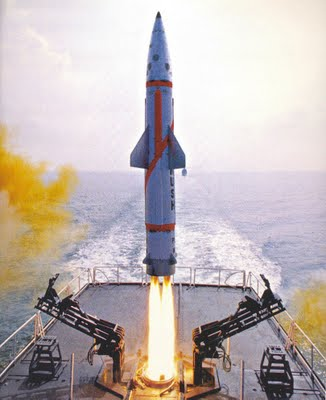
\includegraphics[width=\textwidth,height=0.4\textheight,keepaspectratio]{ballistic_missile.jpg}
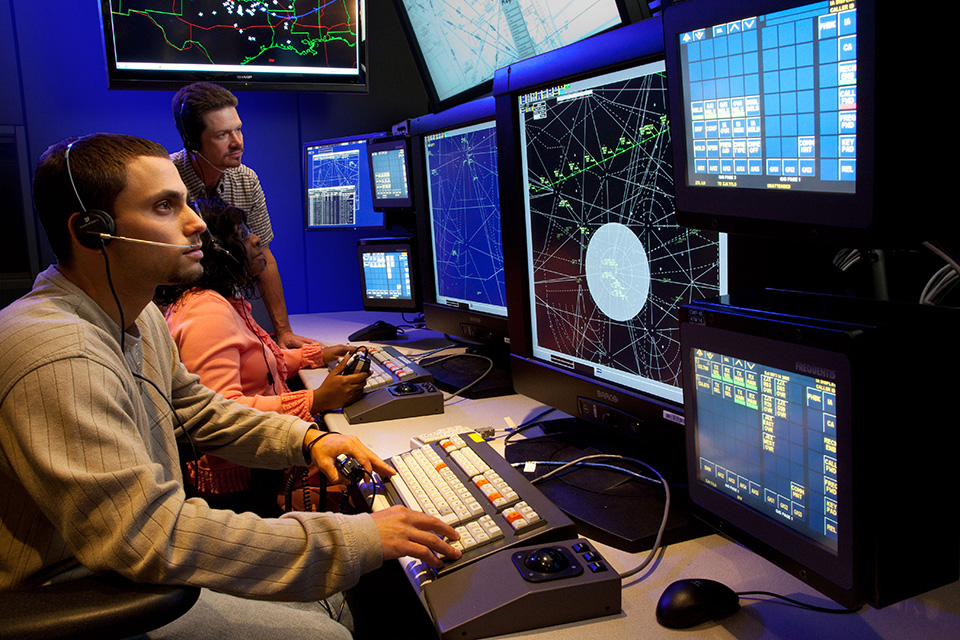
\includegraphics[width=\textwidth,height=0.4\textheight,keepaspectratio]{ATC.jpg}
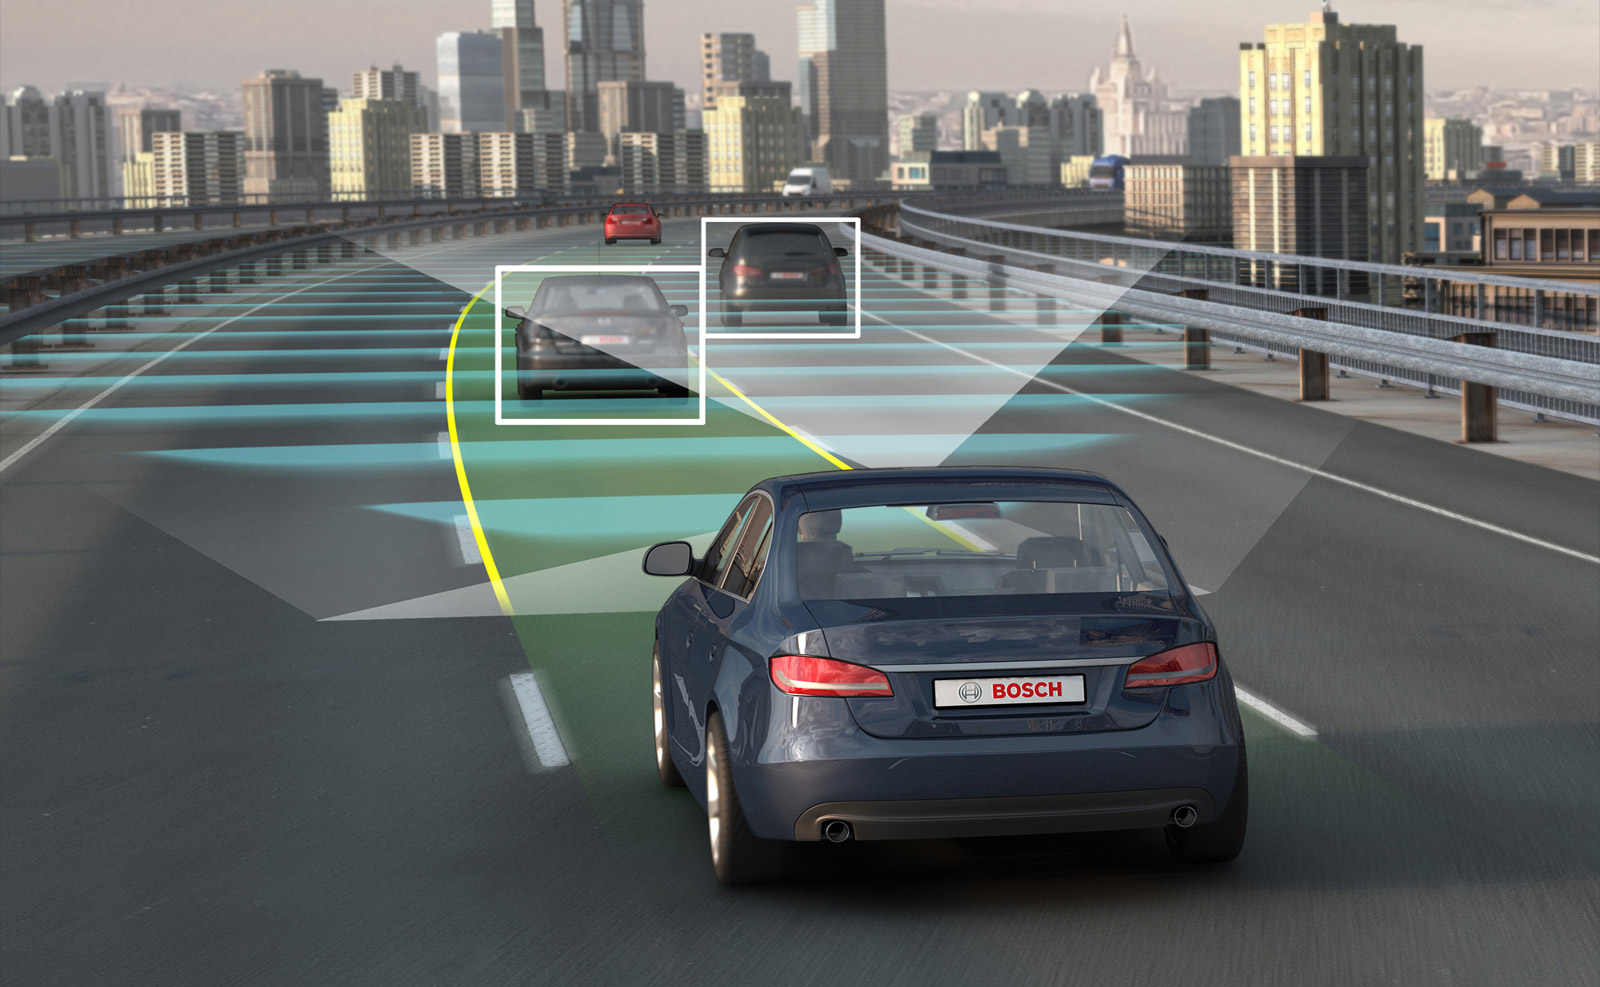
\includegraphics[width=\textwidth,height=0.4\textheight,keepaspectratio]{car.jpg}
\begin{itemize}
\item Ballistic missile and aircraft defense
\item Space applications
\item Movement of ships and ground troops
\item Autonomous vehicles and robotics
\item Air traffic control
\end{itemize}
\end{frame} 

\begin{frame}
\frametitle{Background}
\begin{itemize}
\item Predominantly statistically based approaches
\item Rely on heavy probabilistic assumptions 
\begin{itemize}
\item radar detection process
\item underlying target dynamics/features
\end{itemize}
\item Two most prevalent algorithms: 
\begin{itemize}
\item Multiple Hypothesis Tracker (MHT) 
\item Joint Probability Data Association Filter (JPDAF)
\end{itemize}
\item Little to no emphasis on optimization
\end{itemize}
\end{frame} 

\begin{frame}
\frametitle{Our contributions}
\begin{enumerate}[(i)]
\item Introduce novel approach using MIO models
\item Propose random local search heuristics
\item New measure of complexity and performance
\end{enumerate}
\end{frame}

%------------------------------------------------
\section{Problem Description}
%------------------------------------------------

\begin{frame}
\frametitle{The MTT Problem}
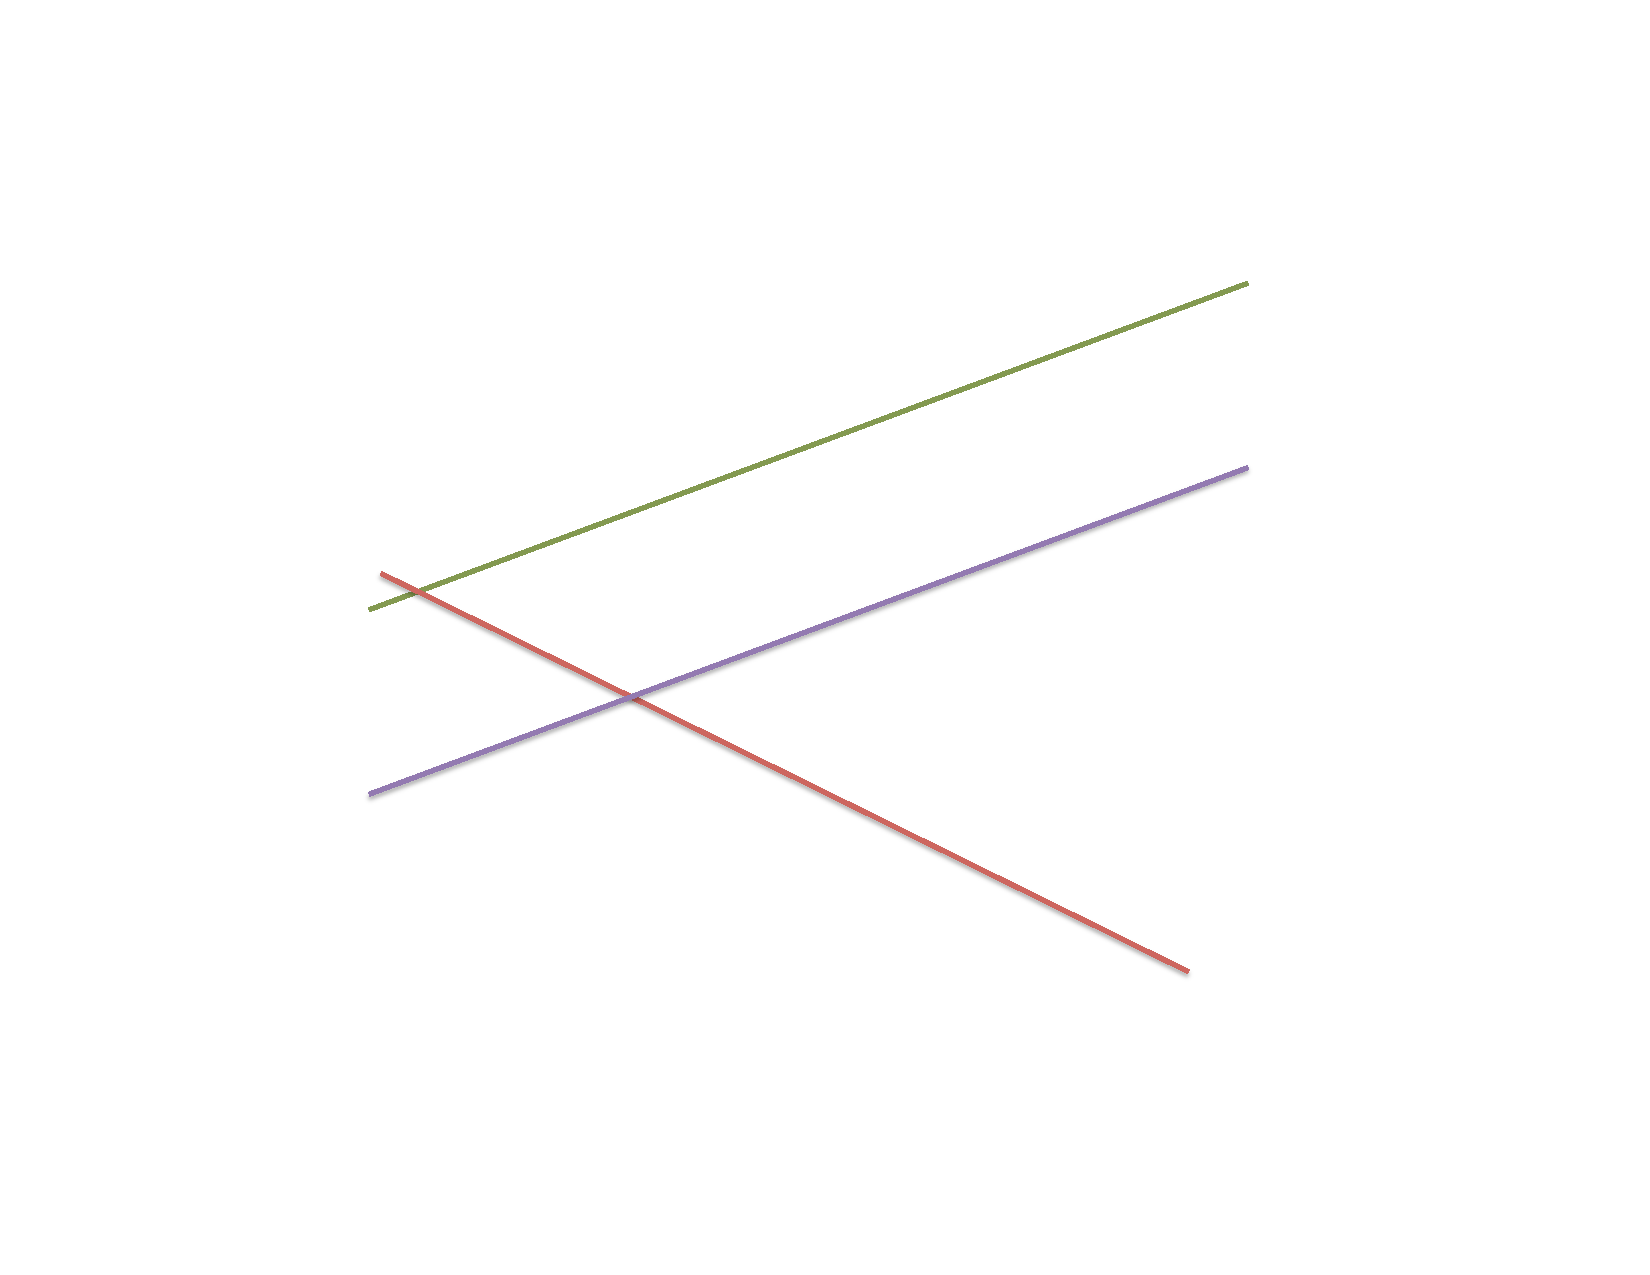
\includegraphics[ width=12cm, height=8cm,keepaspectratio]{Slide_1.pdf}
\end{frame}

\begin{frame}
\frametitle{The MTT Problem}
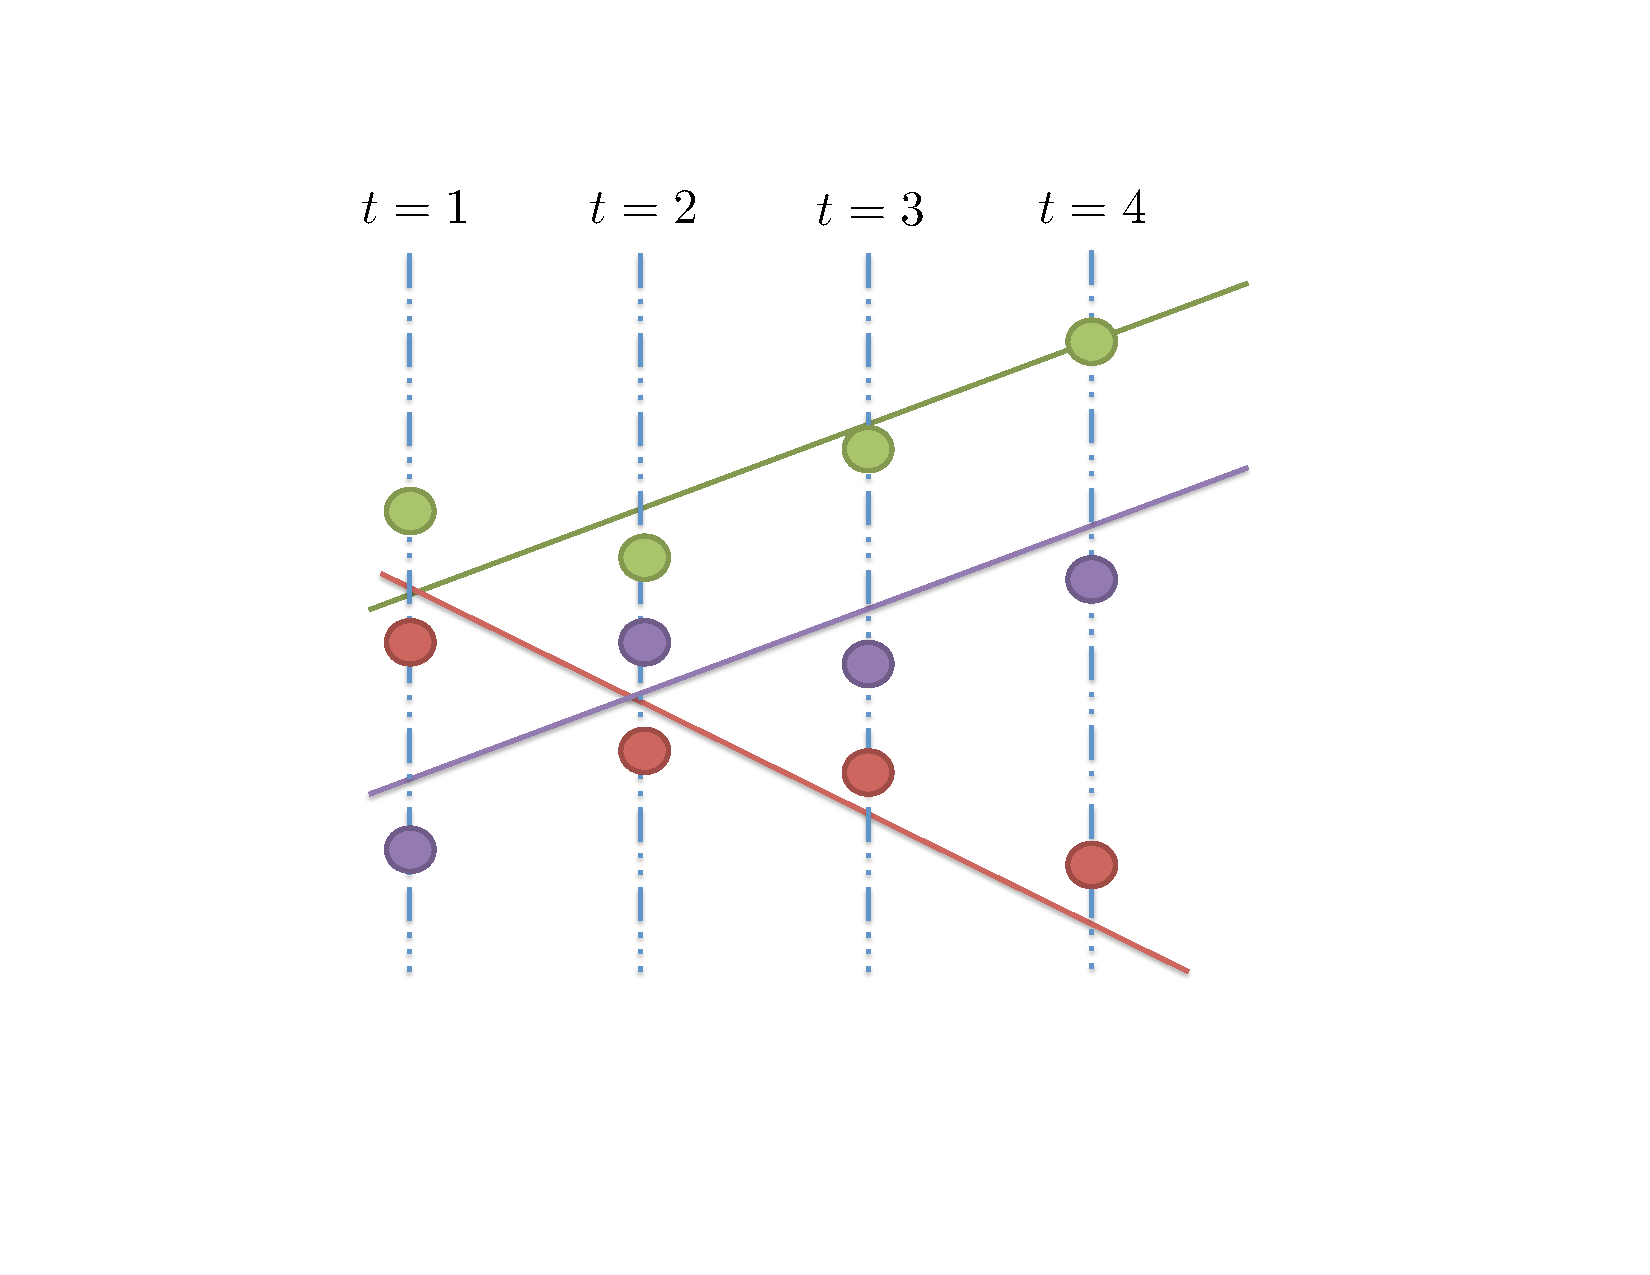
\includegraphics[ width=12cm, height=8cm,keepaspectratio]{Slide_2.pdf}
\end{frame}

\begin{frame}
\frametitle{The MTT Problem}
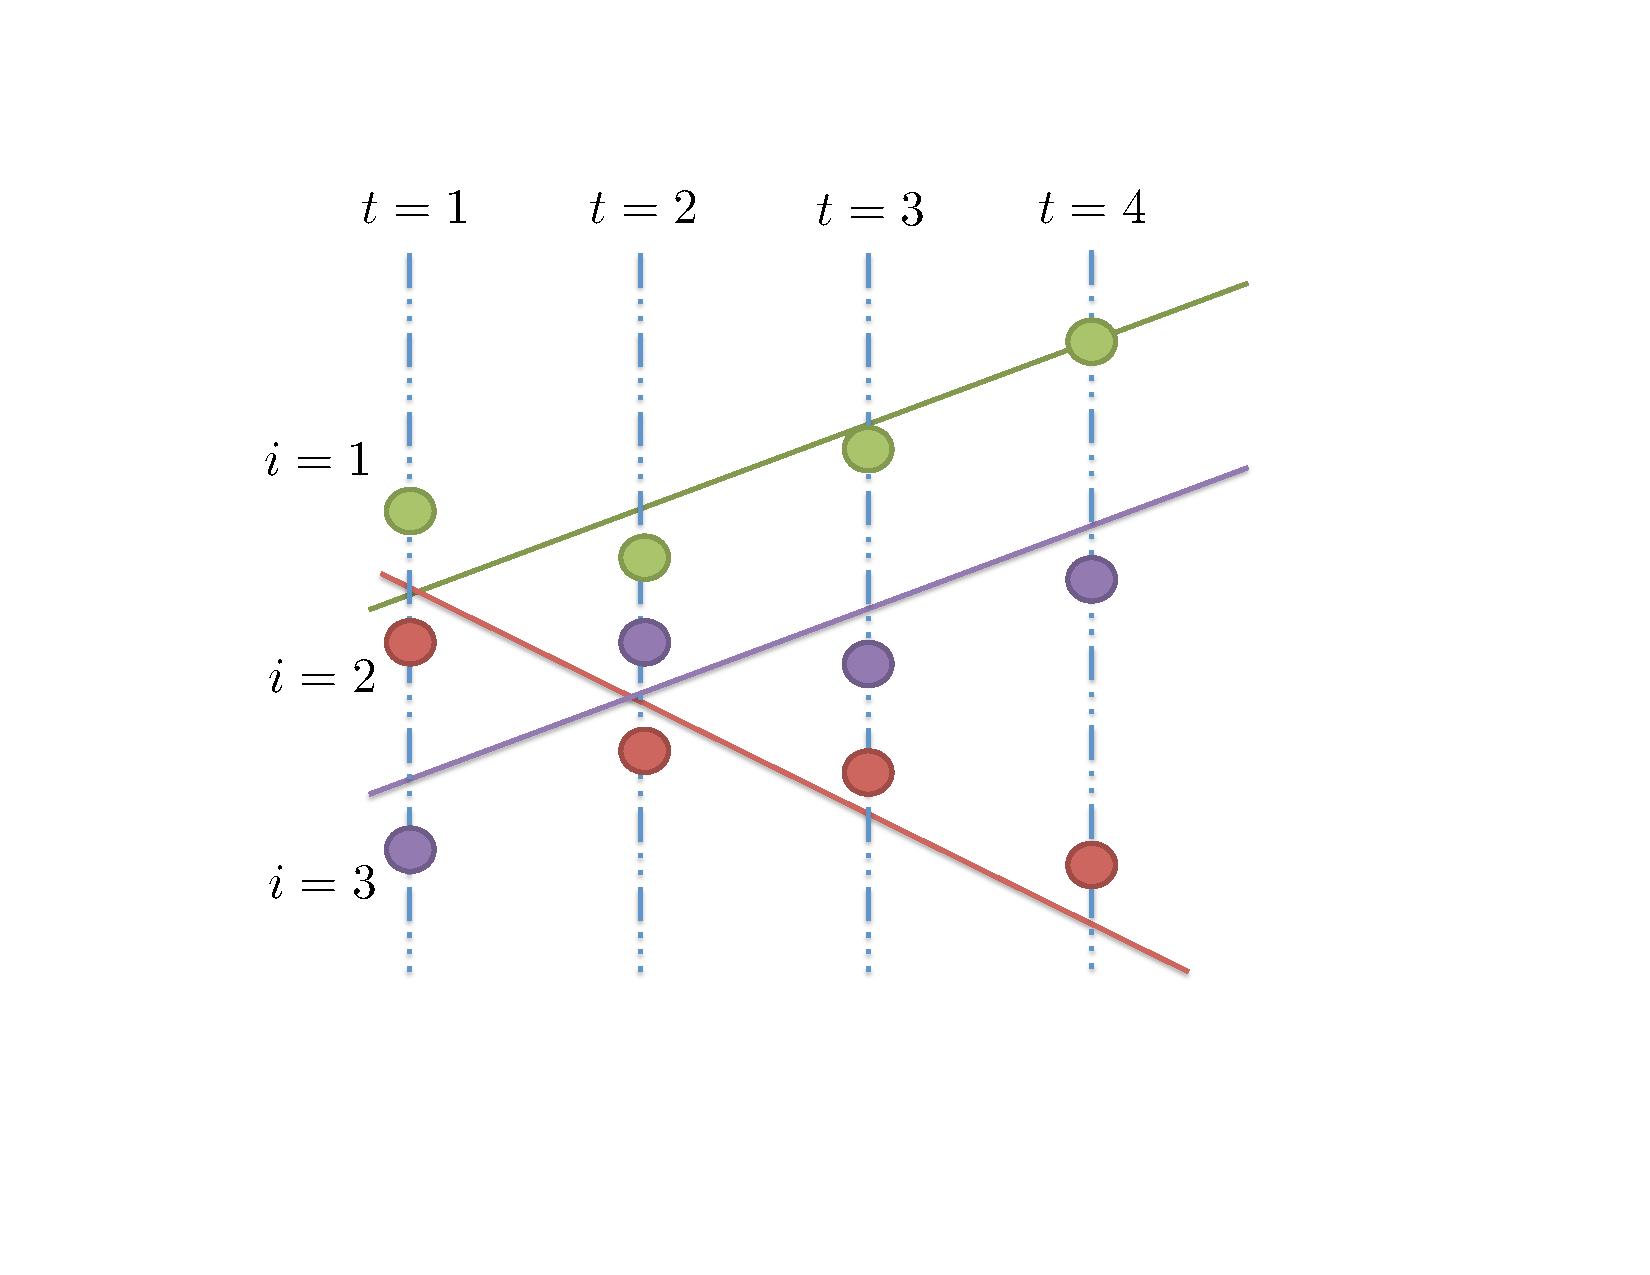
\includegraphics[ width=12cm, height=8cm,keepaspectratio]{Slide_3.pdf}
\end{frame}

\begin{frame}
\frametitle{The MTT Problem}
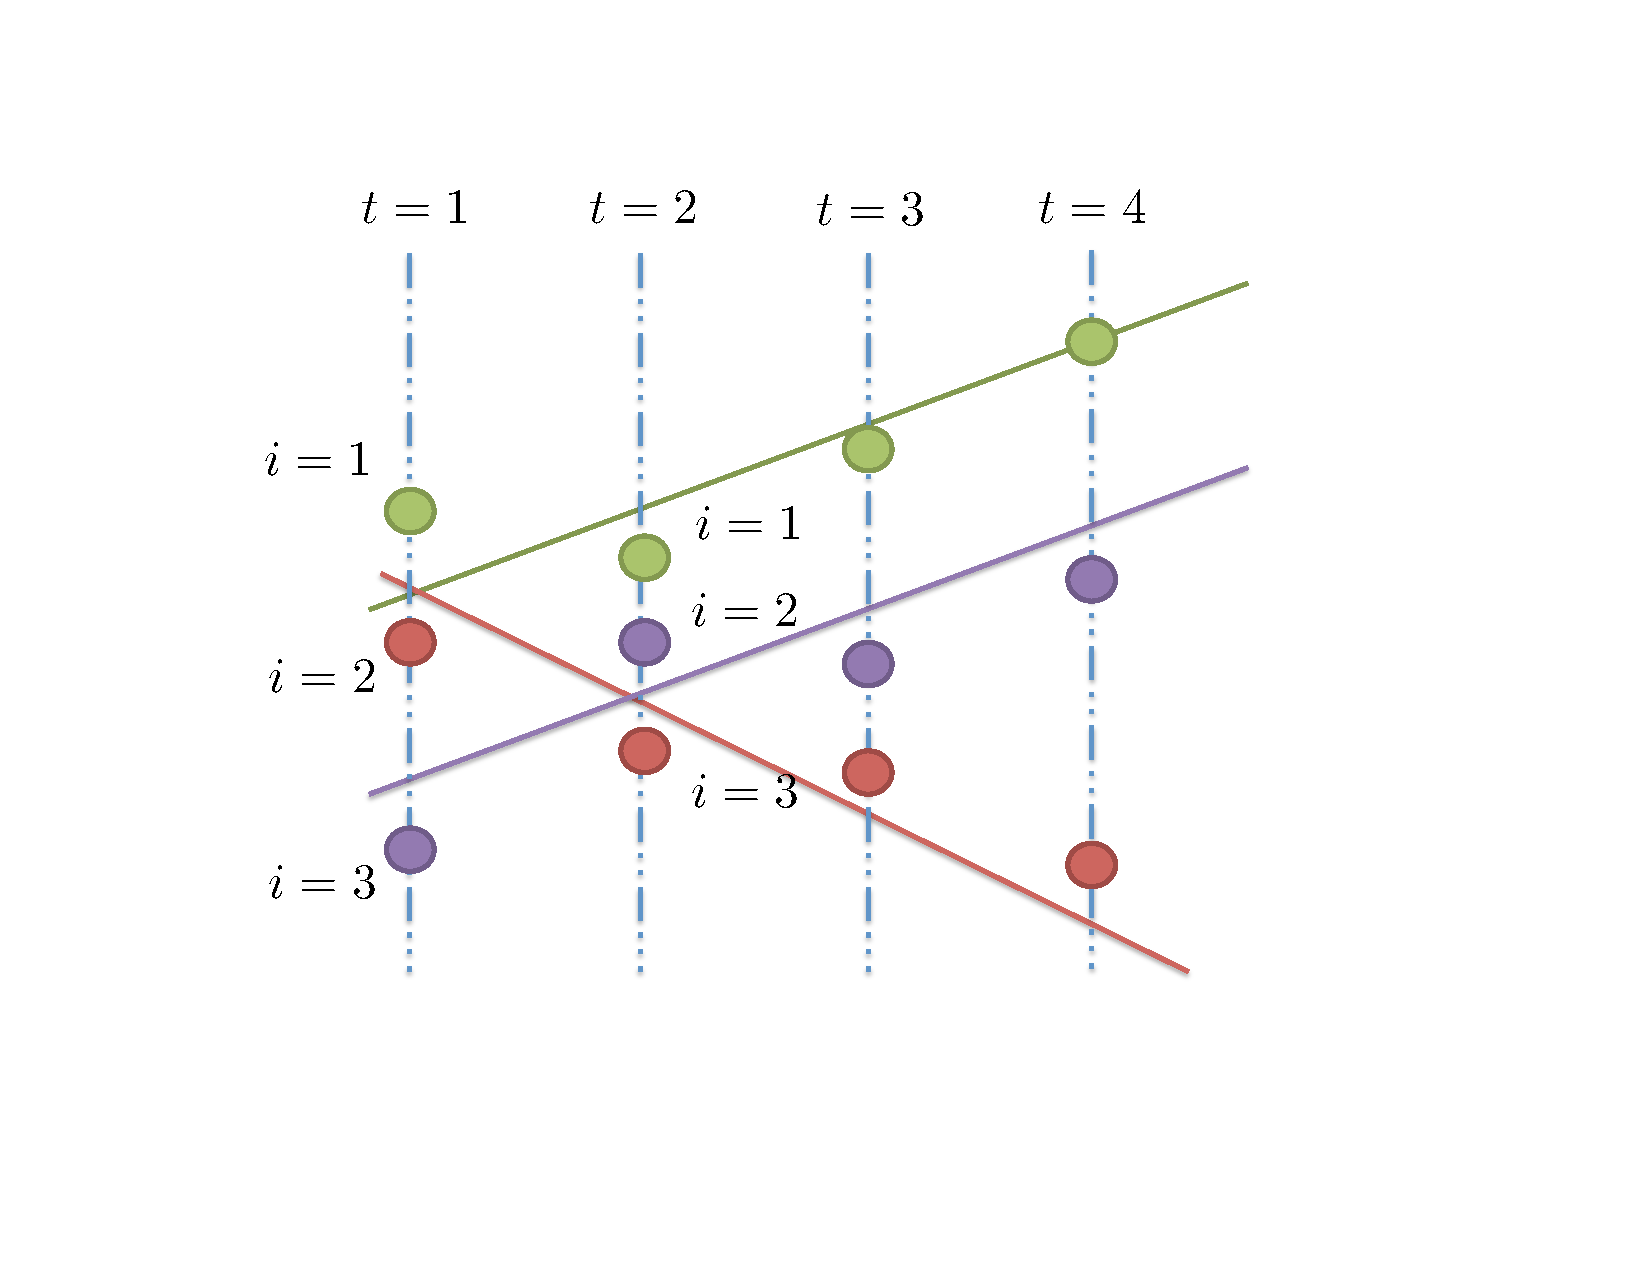
\includegraphics[ width=12cm, height=8cm,keepaspectratio]{Slide_4.pdf}
\end{frame}

\begin{frame}
\frametitle{Notation}
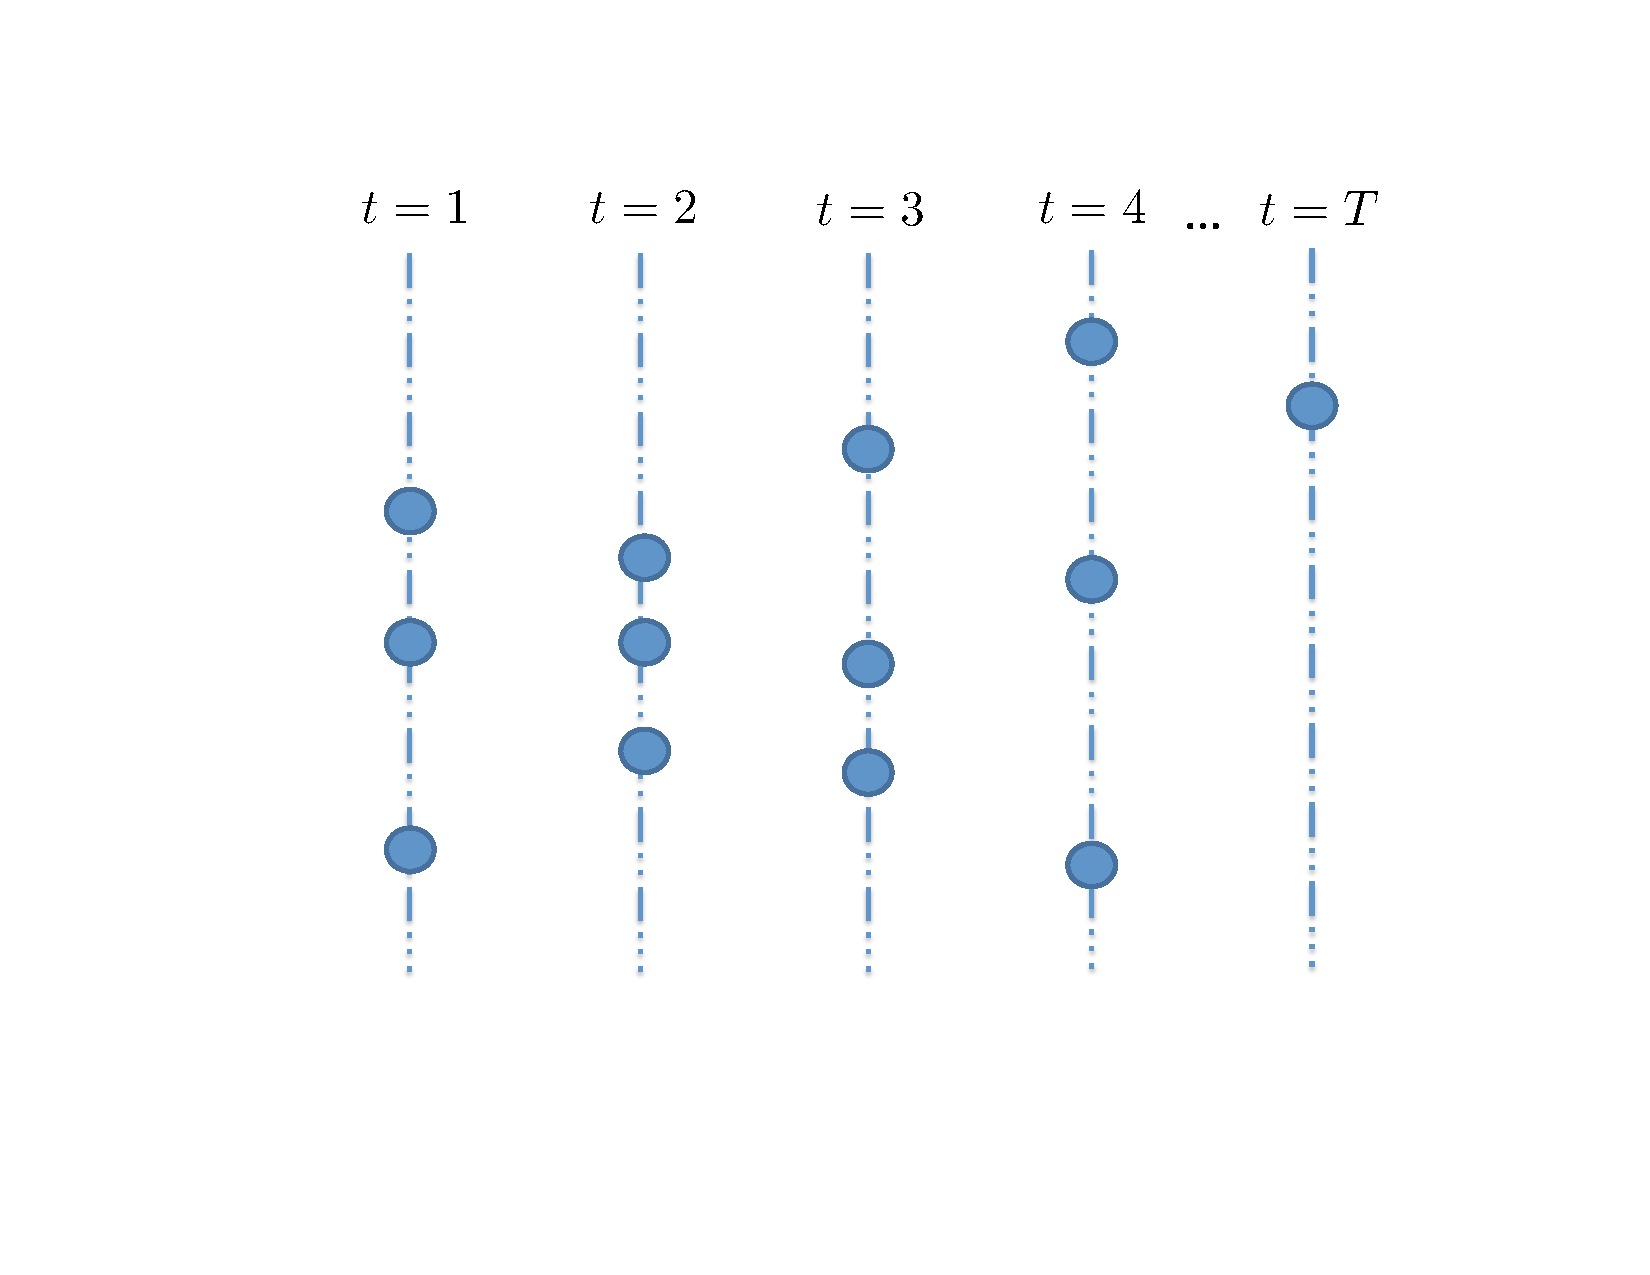
\includegraphics[ width=12cm, height=8cm,keepaspectratio]{Slide_5.pdf}
\end{frame}

\begin{frame}
\frametitle{Notation}
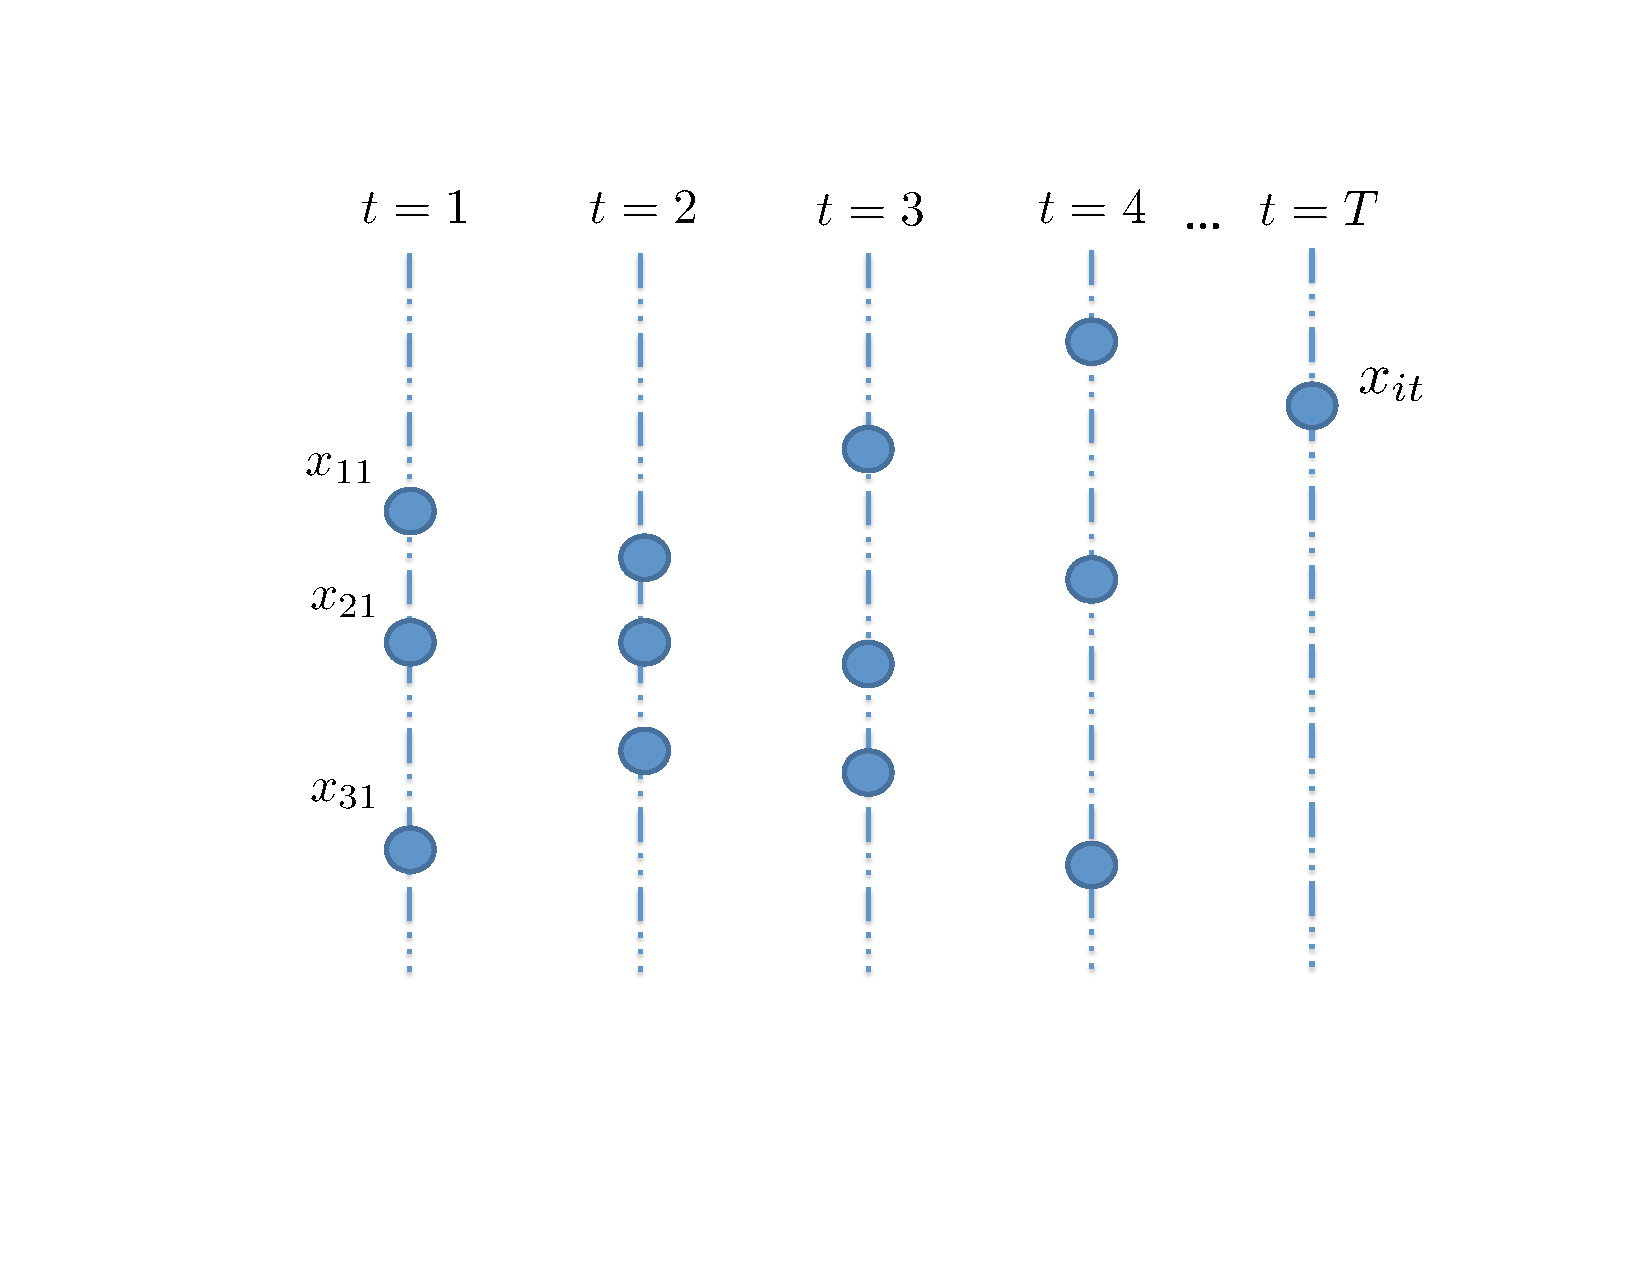
\includegraphics[ width=12cm, height=8cm,keepaspectratio]{Slide_6.pdf}
\end{frame}

\begin{frame}
\frametitle{Notation}
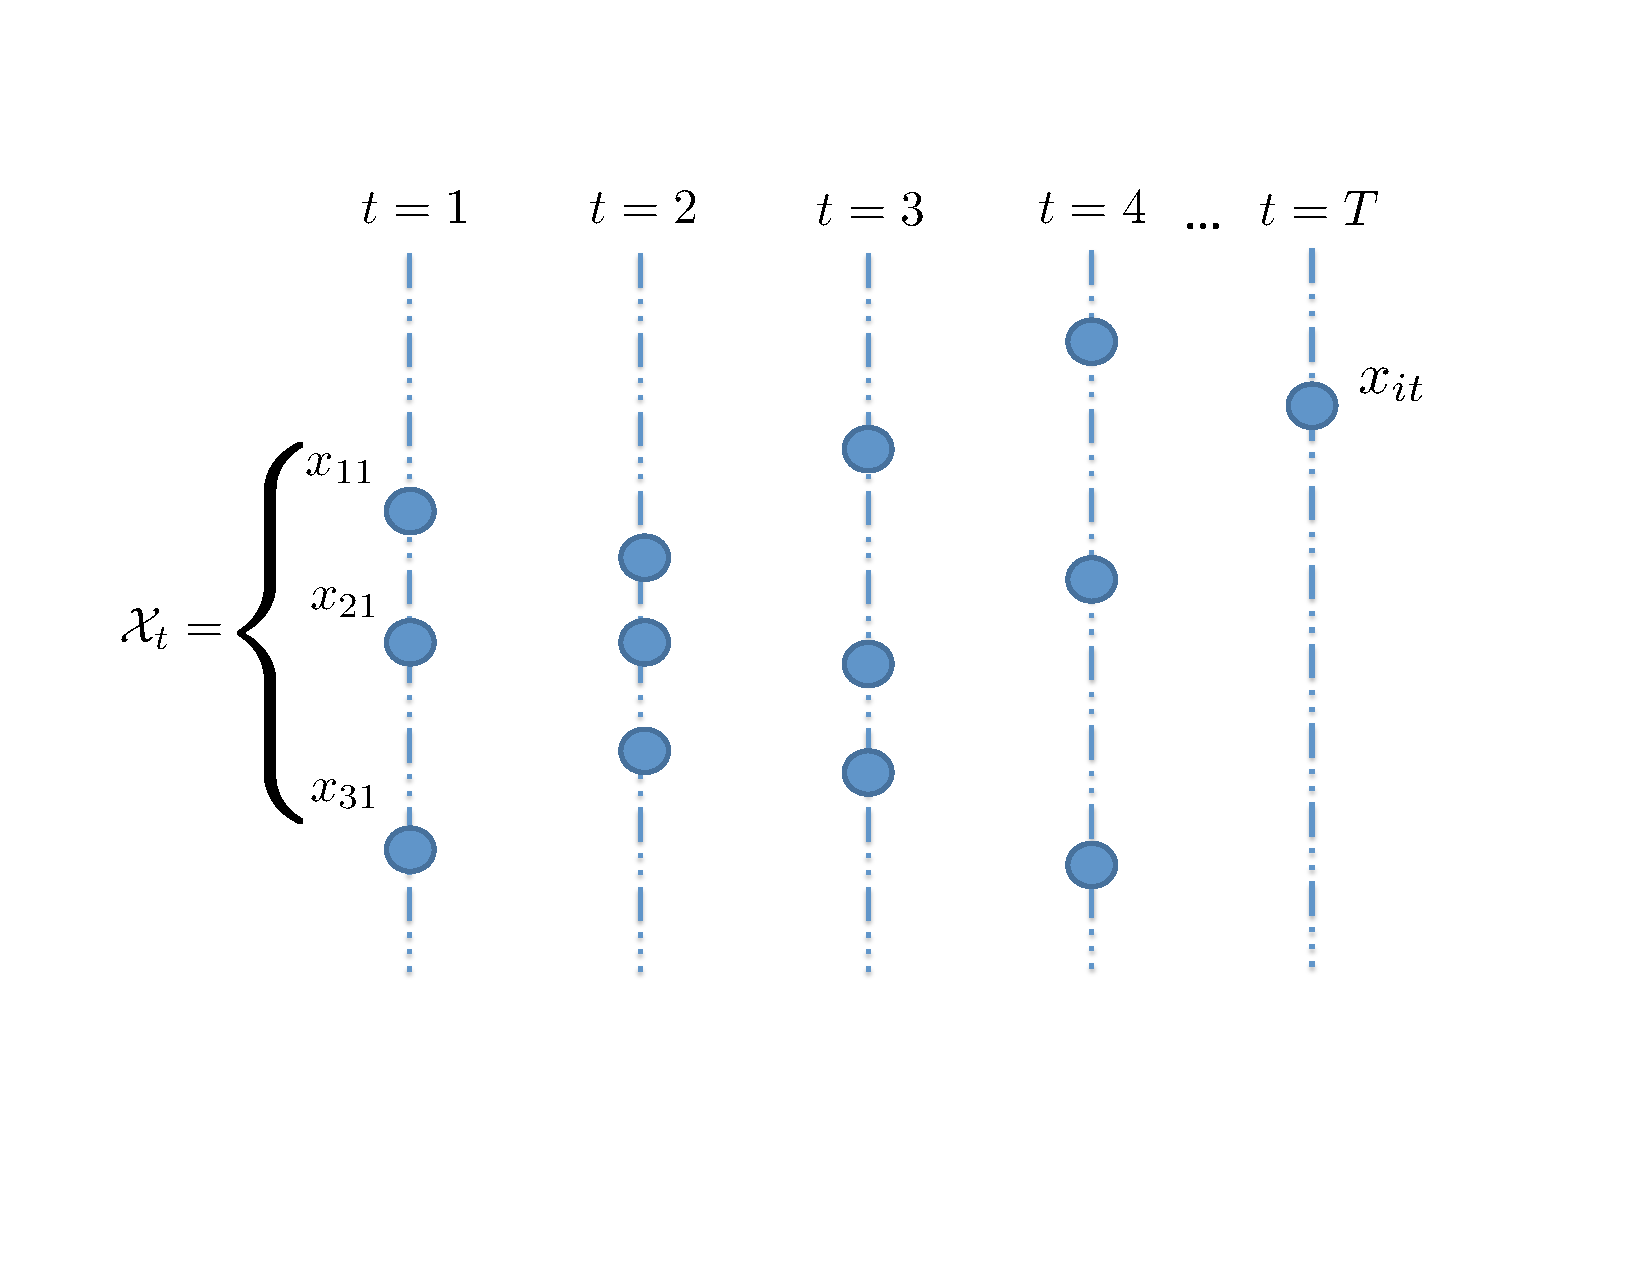
\includegraphics[ width=12cm, height=8cm,keepaspectratio]{Slide_7.pdf}
\end{frame}

\begin{frame}
\frametitle{Notation}
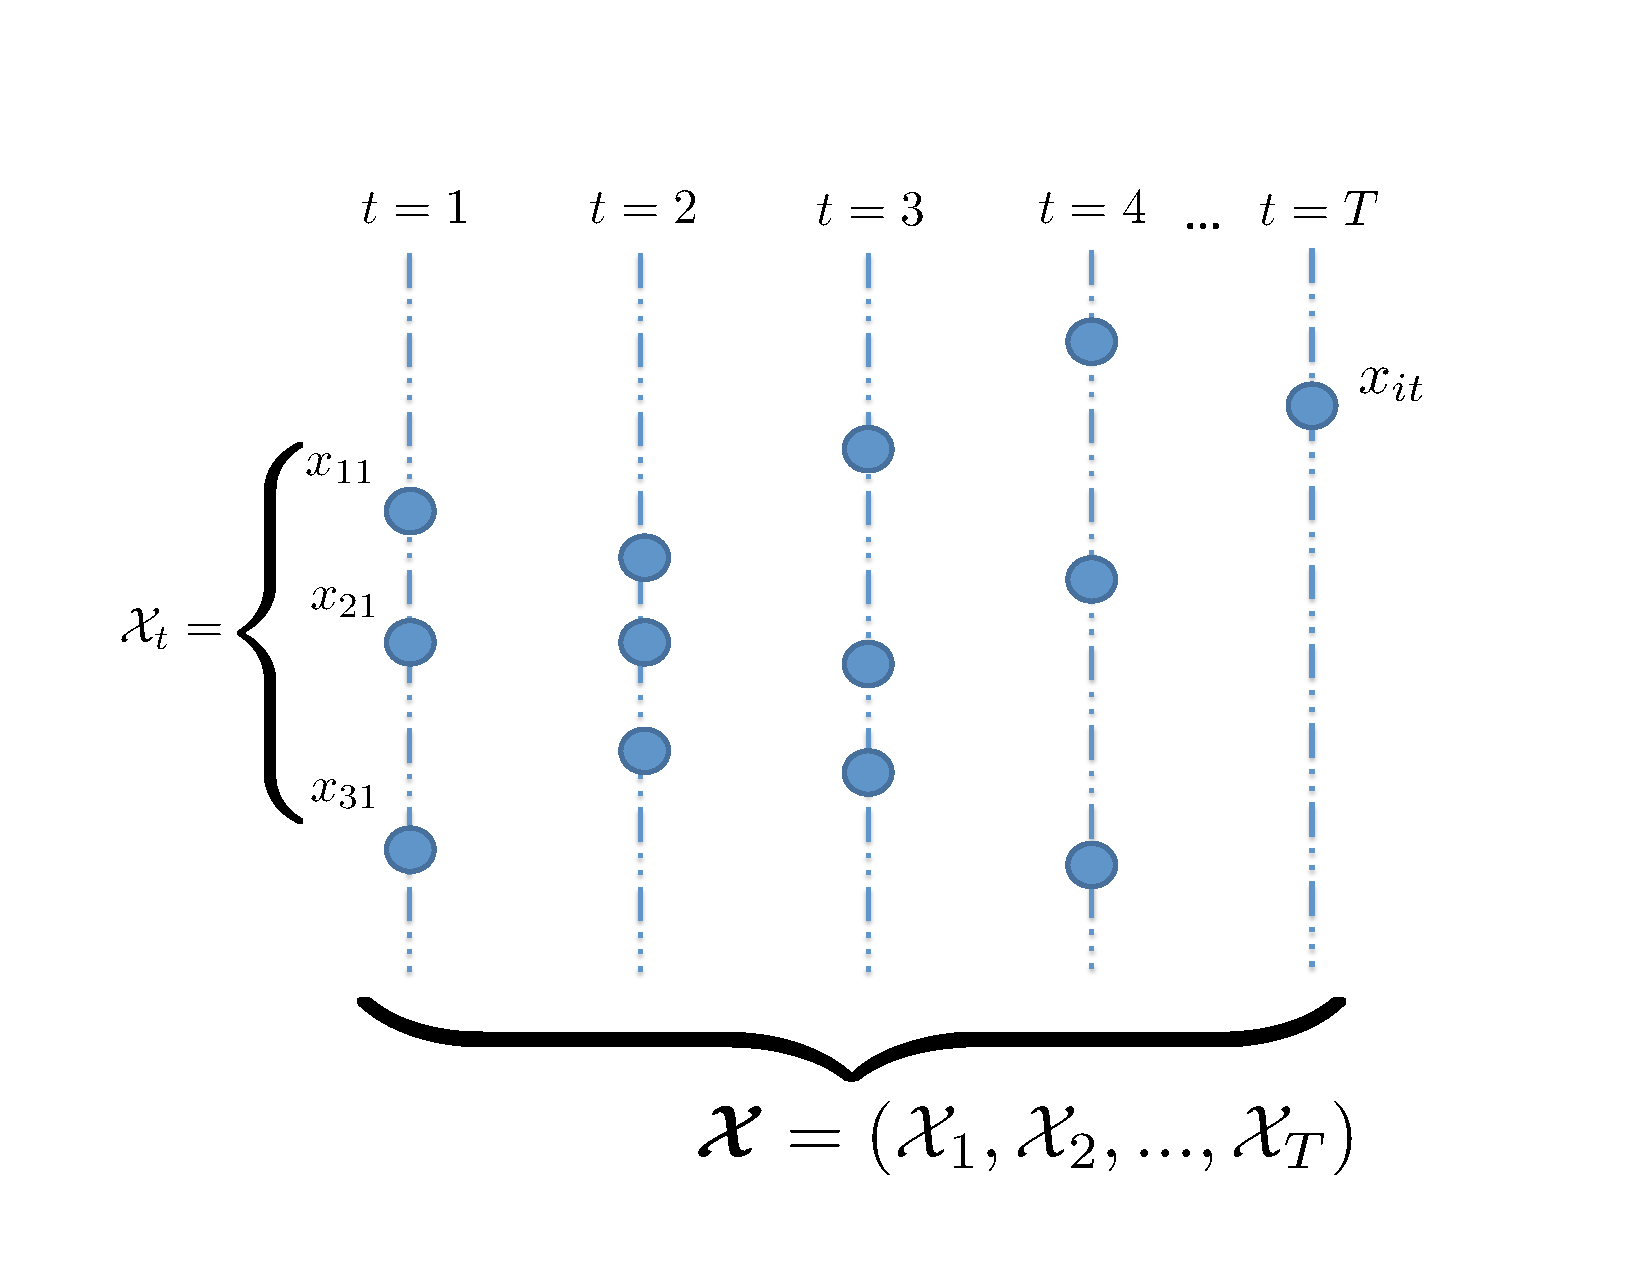
\includegraphics[ width=12cm, height=8cm,keepaspectratio]{Slide_8.pdf}
\end{frame}

\begin{frame}
\frametitle{General Assumptions}
\begin{assumption}
\leavevmode
\begin{enumerate}[(i)]
\item All targets have constant velocity
\item Each target's dynamics are independent 
\item The number of targets remains constant 
\item The detection errors are independent
\end{enumerate}
\end{assumption}
\end{frame} 

%------------------------------------------------
\section{MIO Models}
%------------------------------------------------

\begin{frame}
\frametitle{Assumptions for case of no detection ambiguity}
\begin{assumption}
\leavevmode
\begin{enumerate}[(i)]
\item The sensor generates exactly one detection for each target in each scan i.e., no missed detections.
\item The sensor does not generate any spurious detections
i.e., no false alarms.
\end{enumerate}
\end{assumption}
\begin{corollary}
The number of targets is known/fixed, denoted by $P$
\end{corollary}
\end{frame} 


\begin{frame}
\frametitle{Decision Variables}
Assignment variables:
\newline
\begin{align*}
y_{itj} =
\begin{cases}
1, & \text{if detection $x_{it}$ is assigned to trajectory \textit{j},} \\
0, & \text{otherwise.}
\end{cases}
\end{align*}
\newline
Trajectory estimation variables:
\newline

$\qquad\qquad$Estimated initial position of trajectory $j$: $\alpha_{j} \in \mathbb{R}^n$ \\
$\qquad\qquad$Estimated velocity of trajectory $j$: $\beta_{j} \in \mathbb{R}^n$ 
\end{frame}

\begin{frame}
\frametitle{Objective Function}
\begin{align*}
 \underset{y_{itj}, \alpha_{j}, \beta_{j}}{\text{minimize: }}\sum_{j=1}^{P} \sum_{t=1}^{T}  \left \| \sum_{i=1}^{P}y_{itj}x_{it} - (\alpha_{j} + \beta_{j}t) \right \|
\end{align*}
\begin{itemize}
\item $\sum_{i=1}^{P}y_{itj}x_{it} =$ detection associated with target $j$ at time $t$
\item Measures cost of assignment
\item $\ell_{1}$ vs. $\ell_{2}$
\end{itemize}
\end{frame}

\begin{frame}
\frametitle{Constraints}
For each target and each scan, each detection must be assigned to exactly one target:
\begin{align*}
\sum_{j=1}^{P} y_{itj} = 1 \qquad \forall i,t.
\end{align*}
Similarly, for each scan, each target must be assigned exactly one detection:
\begin{align*}\label{eq:all_targets}
\sum_{i=1}^{P} y_{itj} = 1 \qquad \forall j,t.
\end{align*}
\end{frame}

\begin{frame}[shrink=20]
\frametitle{Overall Formulation}
\begin{align*}
\underset{\psi_{jt}}{\text{minimize: }} & \sum_{j=1}^{P} \sum_{t=1}^{T} \psi_{jt}\\
\text{subject to: }	& \sum_{j=1}^{P} y_{itj} = 1 \qquad \forall i,t\nonumber \\
				& \sum_{i=1}^{P} y_{itj} = 1 \qquad \forall j,t\nonumber \\
				& \sum_{i=1}^{P}y_{itj}x_{it} - \alpha_{j} - \beta_{j}t \leq \psi_{jt} \qquad \forall j,t \nonumber \\
				& -\left(\sum_{i=1}^{P}y_{itj}x_{it} - \alpha_{j} - \beta_{j}t\right) \geq \psi_{jt} \qquad \forall j,t \nonumber \\
			 	& y_{itj} \in \{0,1\} \quad \forall i,t,j \nonumber\\
				& \alpha_{j} \in \mathbb{R}^n \quad \forall j,\quad \beta_{j} \in \mathbb{R}^n \quad \forall j \nonumber
\end{align*}
\end{frame}

\begin{frame}
\frametitle{A need to generalize}
When extending to detection ambiguity, there is no one to one assignment, so 
$$\sum_{i=1}^{P}y_{itj}x_{it} \neq \text{detection associated with target $j$ at time $t$}.$$
\end{frame}

\begin{frame}
\frametitle{Alternate Approach}
\[z_{jt} =
\begin{cases}
x_{it}, & \text{if $y_{itj} = 1$,} \\
\textit{free}, & \text{otherwise.}
\end{cases}\]
\begin{align*}
\underset{z_{jt}, \alpha_{j}, \beta_{j}}{\text{minimize: }} & \sum_{j=1}^{P} \sum_{t=1}^{T} \|z_{jt} - \alpha_{j} - \beta_{j}t\|
\end{align*}
\begin{align*}
M_{t}(1-y_{itj}) \geq |z_{jt} - x_{it}y_{itj}| \qquad \forall i,t,j
\end{align*}
\end{frame}

\begin{frame}[shrink=20]
\frametitle{Generalized Formulation}
\begin{align*}
\underset{\psi_{jt}}{\text{minimize: }} & \sum_{j=1}^{P} \sum_{t=1}^{T} \psi_{jt}\\
\text{subject to: }	& \sum_{j=1}^{P} y_{itj} = 1 \qquad \forall i,t\nonumber\\
				& \sum_{i=1}^{P} y_{itj} = 1 \qquad \forall j,t\nonumber\\
				& x_{it}y_{itj} + M_{t}(1-y_{itj}) \geq z_{jt} \qquad \forall i,t,j\nonumber\\
				& x_{it}y_{itj} - M_{t}(1-y_{itj}) \leq z_{jt} \qquad \forall i,t,j\nonumber\\
				& z_{jt} - \alpha_{j} - \beta_{j}t \leq \psi_{jt} \qquad \forall i,j,t\nonumber\\
				& -(z_{jt} - \alpha_{j} - \beta_{j}t) \geq \psi_{jt} \qquad \forall i,j,t\nonumber\\
			 	& y_{itj} \in \{0,1\} \quad \forall i,t,j\nonumber\\
				& \alpha_{j} \in \mathbb{R}^n \quad \forall j,\quad \beta_{j} \in \mathbb{R}^n \quad \forall j, \quad z_{jt} \in \mathbb{R}^n \quad \forall j,t\nonumber
\end{align*}
\end{frame}


\begin{frame}
\frametitle{Detection Ambiguity - False Alarms}
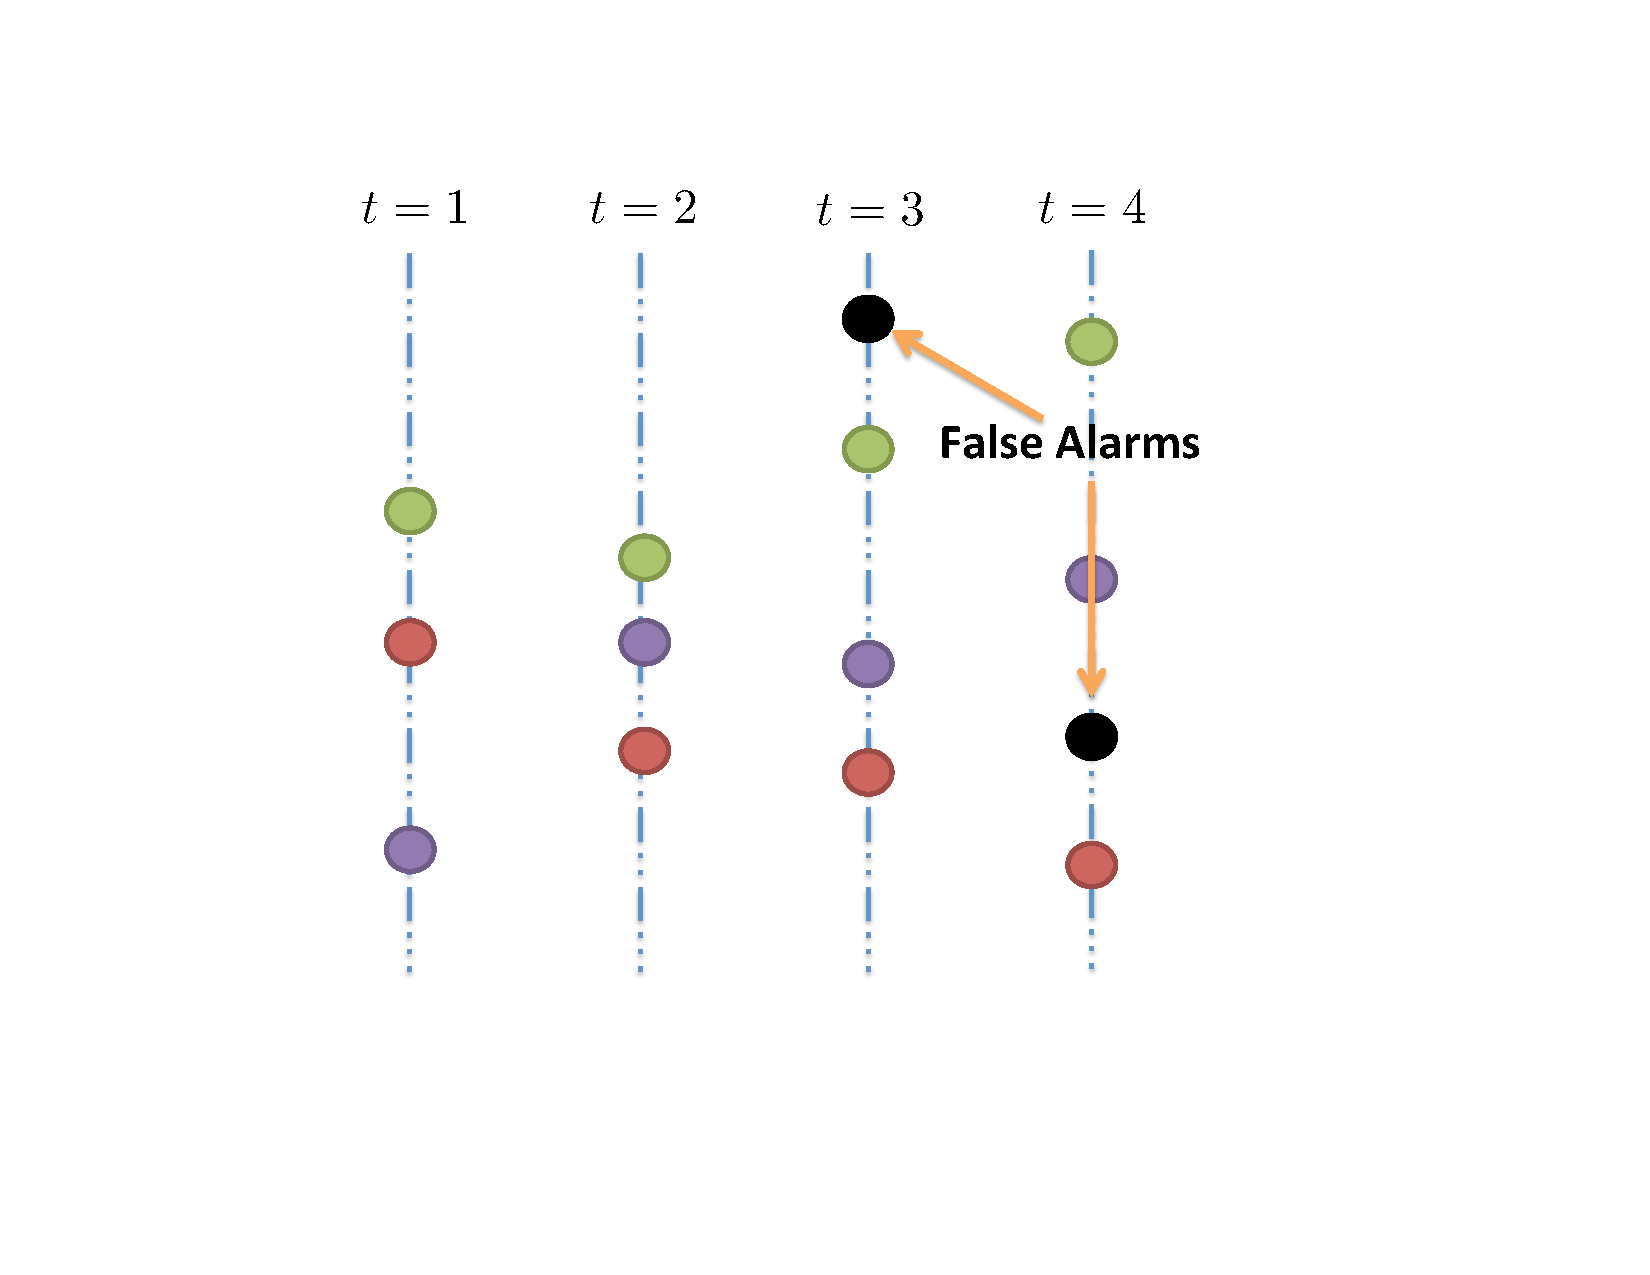
\includegraphics[ width=12cm, height=10cm,keepaspectratio]{Slide_18.pdf}
\end{frame}

\begin{frame}
\frametitle{Detection Ambiguity - Missed Detections}
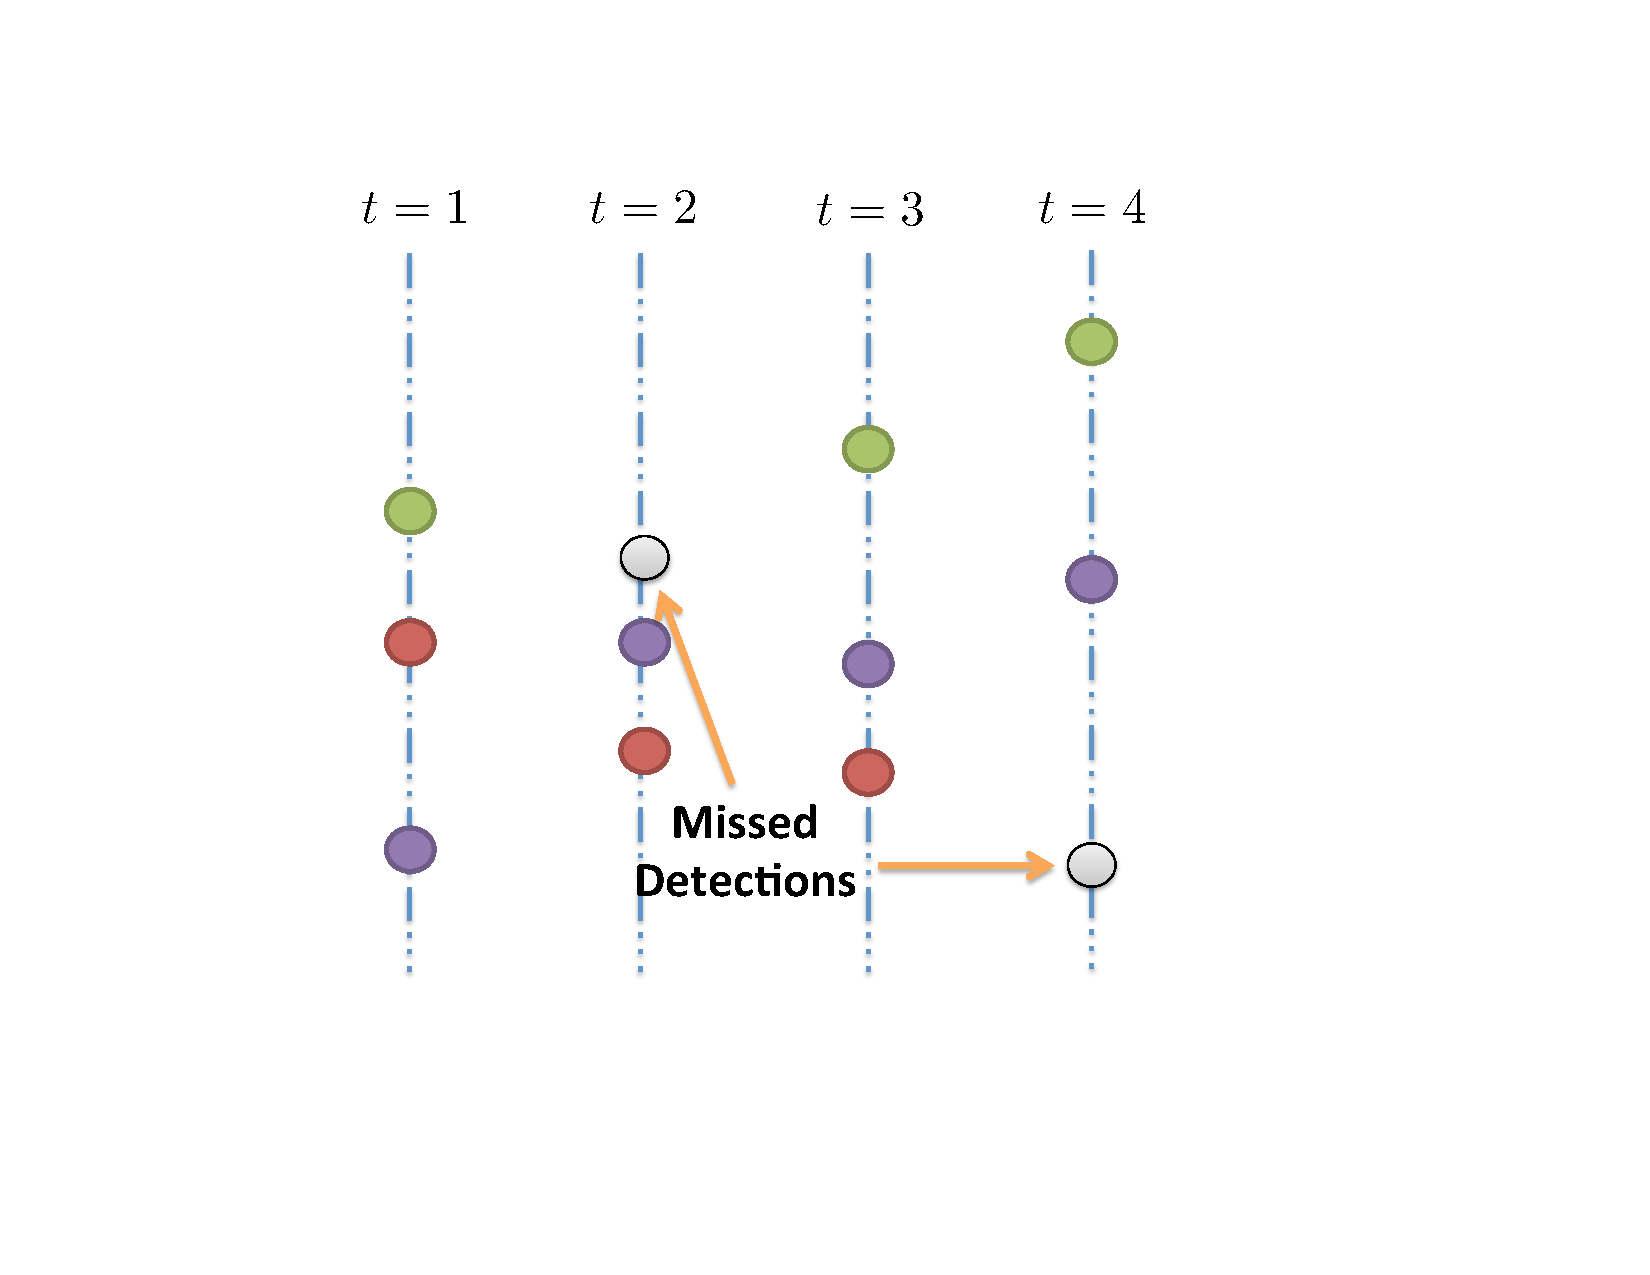
\includegraphics[ width=12cm, height=10cm,keepaspectratio]{Slide_19.pdf}
\end{frame}

\begin{frame}
\frametitle{Detection Ambiguity Notation}
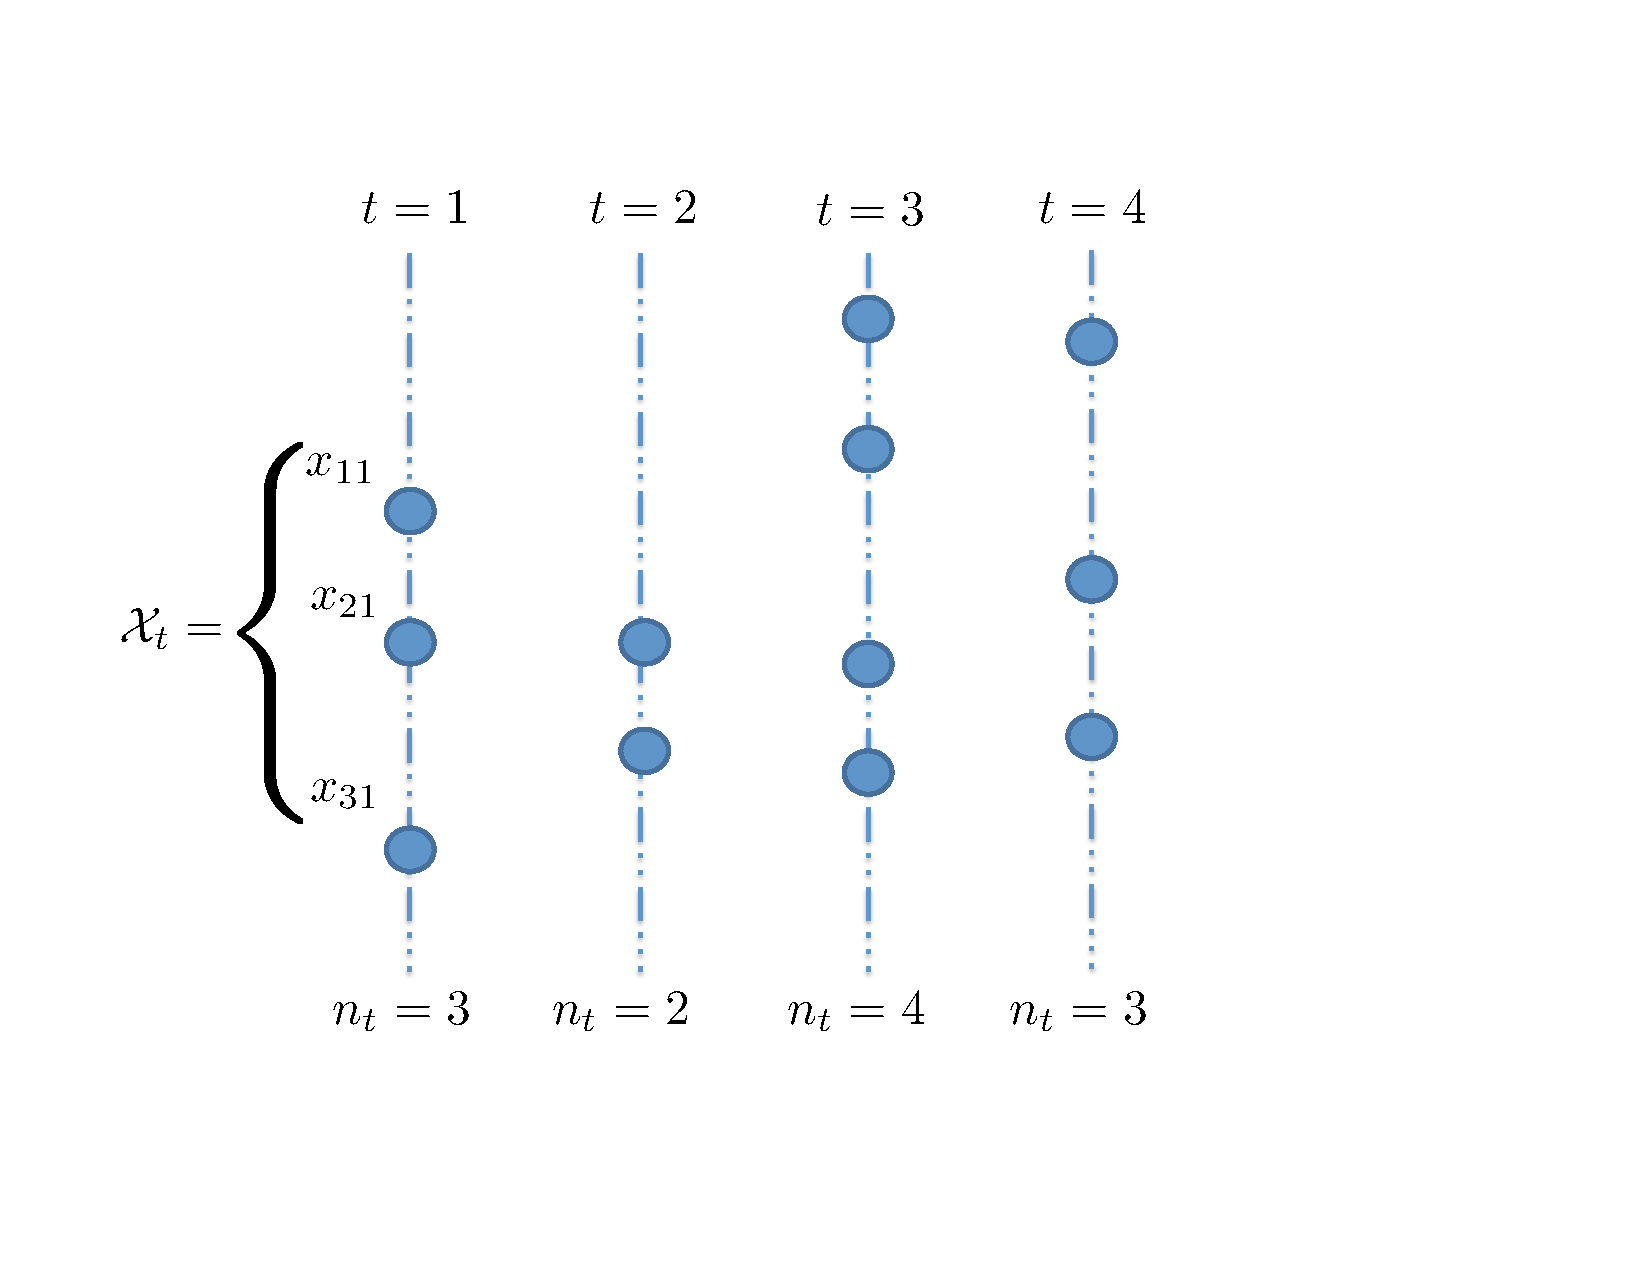
\includegraphics[ width=12cm, height=10cm,keepaspectratio]{Slide_20.pdf}
\end{frame}

\begin{frame}
\frametitle{Assumptions for Case of Detection Ambiguity}
\begin{align*}
N_{0} = \underset{t}{\text{min }} n_{t}
\end{align*}
\begin{align*}
N_{1} = \underset{t}{\text{max }}  n_{t}
\end{align*}
\begin{assumption}
\leavevmode
\begin{enumerate}[(i)]
\item The sensor generates at most one detection for each target in each scan i.e., there can be missed detections.
\item The sensor can generate detections that do not originate from any target i.e., there can be false alarms.
\item The number of true targets $P$ satisfies $N_0\leq P \leq N_1$.
\end{enumerate}
\end{assumption}
\end{frame}

\begin{frame}
\frametitle{How to handle unknown number of targets $P$?}
Two methodologies:
\begin{enumerate}
\item Find optimal $P$ using additional decision variables
\item Find optimal $P$ by:
\begin{itemize}
\item For each $N_0\leq P\leq N_1$ solve problem using MIO for known $P$
\item Choose $P$ with best objective function value
\item Parallelizable 
\end{itemize}
\end{enumerate}
\end{frame}

\begin{frame}
\frametitle{Decision Variables}
False alarms:
\[F_{it} = 
\begin{cases}
1, & \text{if detection \textit{i} at time \textit{t} is a false alarm,}\\
0, & \text{otherwise.}
\end{cases}\]
Missed Detections:
\[M_{jt} =
\begin{cases}
1, & \text{if detection for trajectory \textit{j} at time \textit{t} is}\\
   &\text{a missed detection,}\\
0, & \text{otherwise.}
\end{cases}\]
\end{frame}

\begin{frame}[shrink=20]
\frametitle{Generalized Formulation}
\begin{align*}
\underset{\psi_{jt}}{\text{minimize: }} & \sum_{j=1}^{P} \sum_{t=1}^{T} \psi_{jt}\\
\text{subject to: }	& \sum_{j=1}^{P} y_{itj} = 1 \qquad \forall i,t\nonumber\\
				& \sum_{i=1}^{P} y_{itj} = 1 \qquad \forall j,t\nonumber\\
				& x_{it}y_{itj} + M_{t}(1-y_{itj}) \geq z_{jt} \qquad \forall i,t,j\nonumber\\
				& x_{it}y_{itj} - M_{t}(1-y_{itj}) \leq z_{jt} \qquad \forall i,t,j\nonumber\\
				& z_{jt} - \alpha_{j} - \beta_{j}t \leq \psi_{jt} \qquad \forall i,j,t\nonumber\\
				& -(z_{jt} - \alpha_{j} - \beta_{j}t) \geq \psi_{jt} \qquad \forall i,j,t\nonumber\\
			 	& y_{itj} \in \{0,1\} \quad \forall i,t,j\\
				& \alpha_{j} \in \mathbb{R}^n \quad \forall j,\quad \beta_{j} \in \mathbb{R}^n \quad \forall j, \quad z_{jt} \in \mathbb{R}^n \quad \forall j,t\nonumber
\end{align*}
\end{frame}

\begin{frame}[shrink=20]
\frametitle{Modification of Constraints}
\begin{align*}
\underset{\psi_{jt}}{\text{minimize: }} & \sum_{j=1}^{P} \sum_{t=1}^{T} \psi_{jt} \\
\text{subject to: }	& \sum_{j=1}^{P} y_{itj} {\color{red}+ F_{it}} = 1 \qquad \forall i,t\nonumber \\
				& \sum_{i=1}^{{\color{red}n_{t}}} y_{itj} + {\color{red}M_{jt}} = 1 \qquad \forall j,t \\
				& x_{it}y_{itj} + M_{t}(1-y_{itj}) \geq z_{jt} \qquad \forall i,t,j\nonumber\\
				& x_{it}y_{itj} - M_{t}(1-y_{itj}) \leq z_{jt} \qquad \forall i,t,j\nonumber\\
				& z_{jt} - \alpha_{j} - \beta_{j}t \leq \psi_{jt} \qquad \forall i,j,t\nonumber\\
				& -(z_{jt} - \alpha_{j} - \beta_{j}t) \geq \psi_{jt} \qquad \forall i,j,t\nonumber\\
			 	& y_{itj} \in \{0,1\} \quad \forall i,t,j, \color{red}{\quad F_{it} \in \{0,1\} \quad \forall i,t,\quad M_{jt} \in \{0,1\} \quad \forall j,t}\\
				& \alpha_{j} \in \mathbb{R}^n \quad \forall j,\quad \beta_{j} \in \mathbb{R}^n \quad \forall j, \quad z_{jt} \in \mathbb{R}^n \quad \forall j,t,
\end{align*}
\end{frame}


\begin{frame}[shrink=20]
\frametitle{Changes to Objective Function}
\begin{align*}
\underset{\psi_{jt}}{\text{minimize: }} & \sum_{j=1}^{P} \sum_{t=1}^{T} \psi_{jt} \color{red}{+ \theta \cdot TF + \phi \cdot TM} \\
\text{subject to: }	& \sum_{j=1}^{P} y_{itj} + F_{it} = 1 \qquad \forall i,t \nonumber \\
				& \sum_{i=1}^{n_{t}} y_{itj} + M_{jt} = 1 \qquad \forall j,t \nonumber\\
				& \color{red}{\sum_{i=1}^{n_{t}} \sum_{t=1}^{T} F_{it} = TF} \nonumber \\
				& \color{red}{\sum_{j=1}^{P} \sum_{t=1}^{T} M_{jt} = TM} \nonumber \\
				& x_{it}y_{itj} + M_{t}(1-y_{itj}) \geq z_{jt} \qquad \forall i,t,j\nonumber\\
				& x_{it}y_{itj} - M_{t}(1-y_{itj}) \leq z_{jt} \qquad \forall i,t,j\nonumber\\
				& z_{jt} - \alpha_{j} - \beta_{j}t \leq \psi_{jt} \qquad \forall i,j,t\nonumber\\
				& -(z_{jt} - \alpha_{j} - \beta_{j}t) \geq \psi_{jt} \qquad \forall i,j,t\nonumber\\
			 	& y_{itj} \in \{0,1\} \quad \forall i,t,j, \quad F_{it} \in \{0,1\} \quad \forall i,t,\quad M_{jt} \in \{0,1\} \quad \forall j,t\\
				& \alpha_{j} \in \mathbb{R}^n \quad \forall j,\quad \beta_{j} \in \mathbb{R}^n \quad \forall j,\quad z_{jt} \in \mathbb{R}^n \quad \forall j,t,\quad \color{red}{TF \in \mathbb{R}^n,TM \in \mathbb{R}^n}\nonumber
\end{align*}
\end{frame}

\begin{frame}[shrink=20]
\frametitle{Robust MIO Model}
\begin{align*}
\underset{\psi_{jt}}{\text{minimize: }} & \sum_{j=1}^{P} \sum_{t=1}^{T} \psi_{jt} + \theta \cdot TF + \phi \cdot TM \\
\text{subject to: }	& \sum_{j=1}^{P} y_{itj} + F_{it} = 1 \qquad \forall i,t \nonumber \\
				& \sum_{i=1}^{n_{t}} y_{itj} + M_{jt} = 1 \qquad \forall j,t \nonumber\\
				& \sum_{i=1}^{n_{t}} \sum_{t=1}^{T} F_{it} = TF \nonumber \\
				& \sum_{j=1}^{P} \sum_{t=1}^{T} M_{jt} = TM \nonumber \\
				& x_{it}y_{itj} + M_{t}(1-y_{itj}) \geq z_{jt} \qquad \forall i,t,j \nonumber \\
				& x_{it}y_{itj} - M_{t}(1-y_{itj}) \leq z_{jt} \qquad \forall i,t,j \nonumber \\
				& z_{jt} - \alpha_{j} - \beta_{j}t \leq \psi_{jt} \qquad \forall j,t \nonumber \\
				& -(z_{jt} - \alpha_{j} - \beta_{j}t) \leq \psi_{jt} \qquad \forall j,t \nonumber \\
			 	& y_{itj} \in \{0,1\} \quad \forall i,t,j,\quad F_{it} \in \{0,1\} \quad \forall i,t,\quad M_{jt} \in \{0,1\} \quad \forall j,t\\
				& \alpha_{j} \in \mathbb{R}^n \quad \forall j,\quad \beta_{j} \in \mathbb{R}^n \quad \forall j, \quad z_{jt} \in \mathbb{R}^n \quad \forall j,t,\quad TF \in \mathbb{R}^n,TM \in \mathbb{R}^n\end{align*}
\end{frame}

%------------------------------------------------
\section{Randomized Local Search Heuristics}
%------------------------------------------------

\begin{frame}
\frametitle{Original Problem Data}
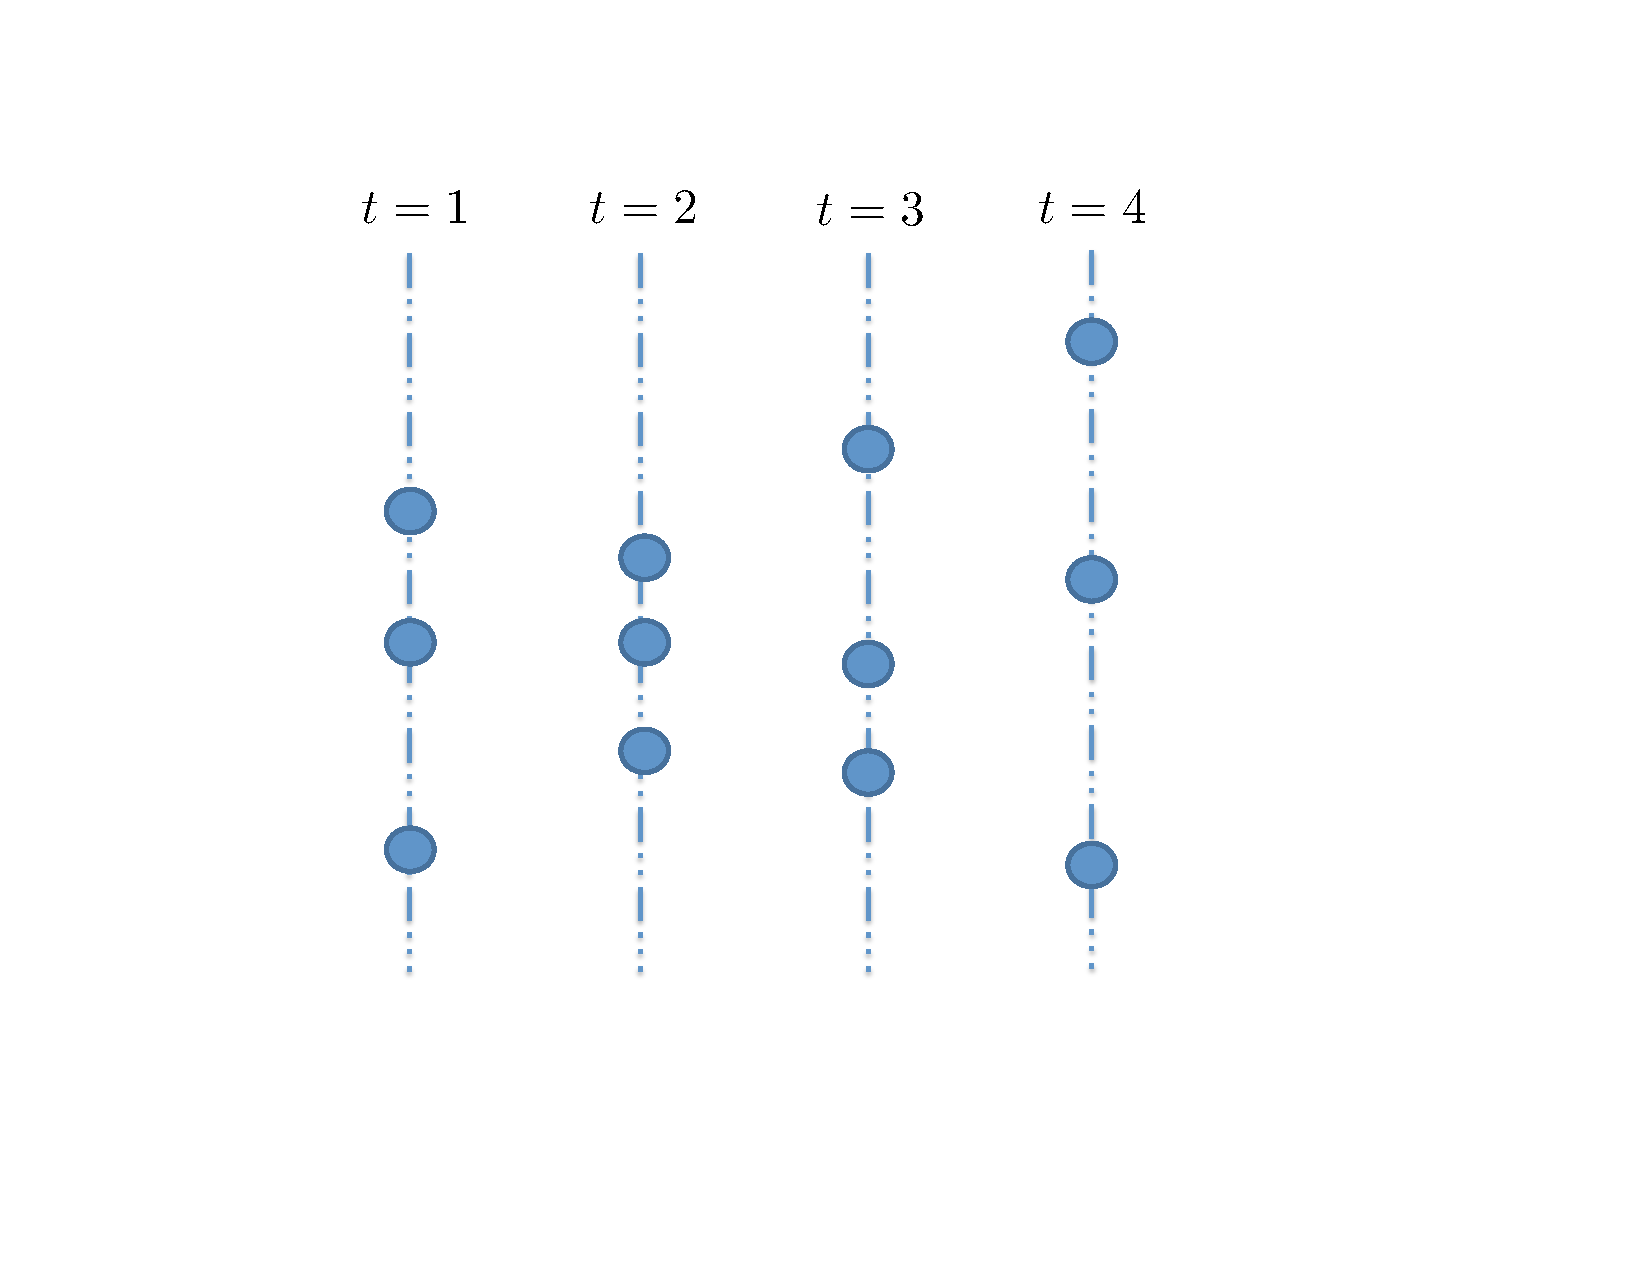
\includegraphics[ width=12cm, height=10cm,keepaspectratio]{Slide_9.pdf}
\end{frame}

\begin{frame}
\frametitle{Randomize Initial Starting Point}
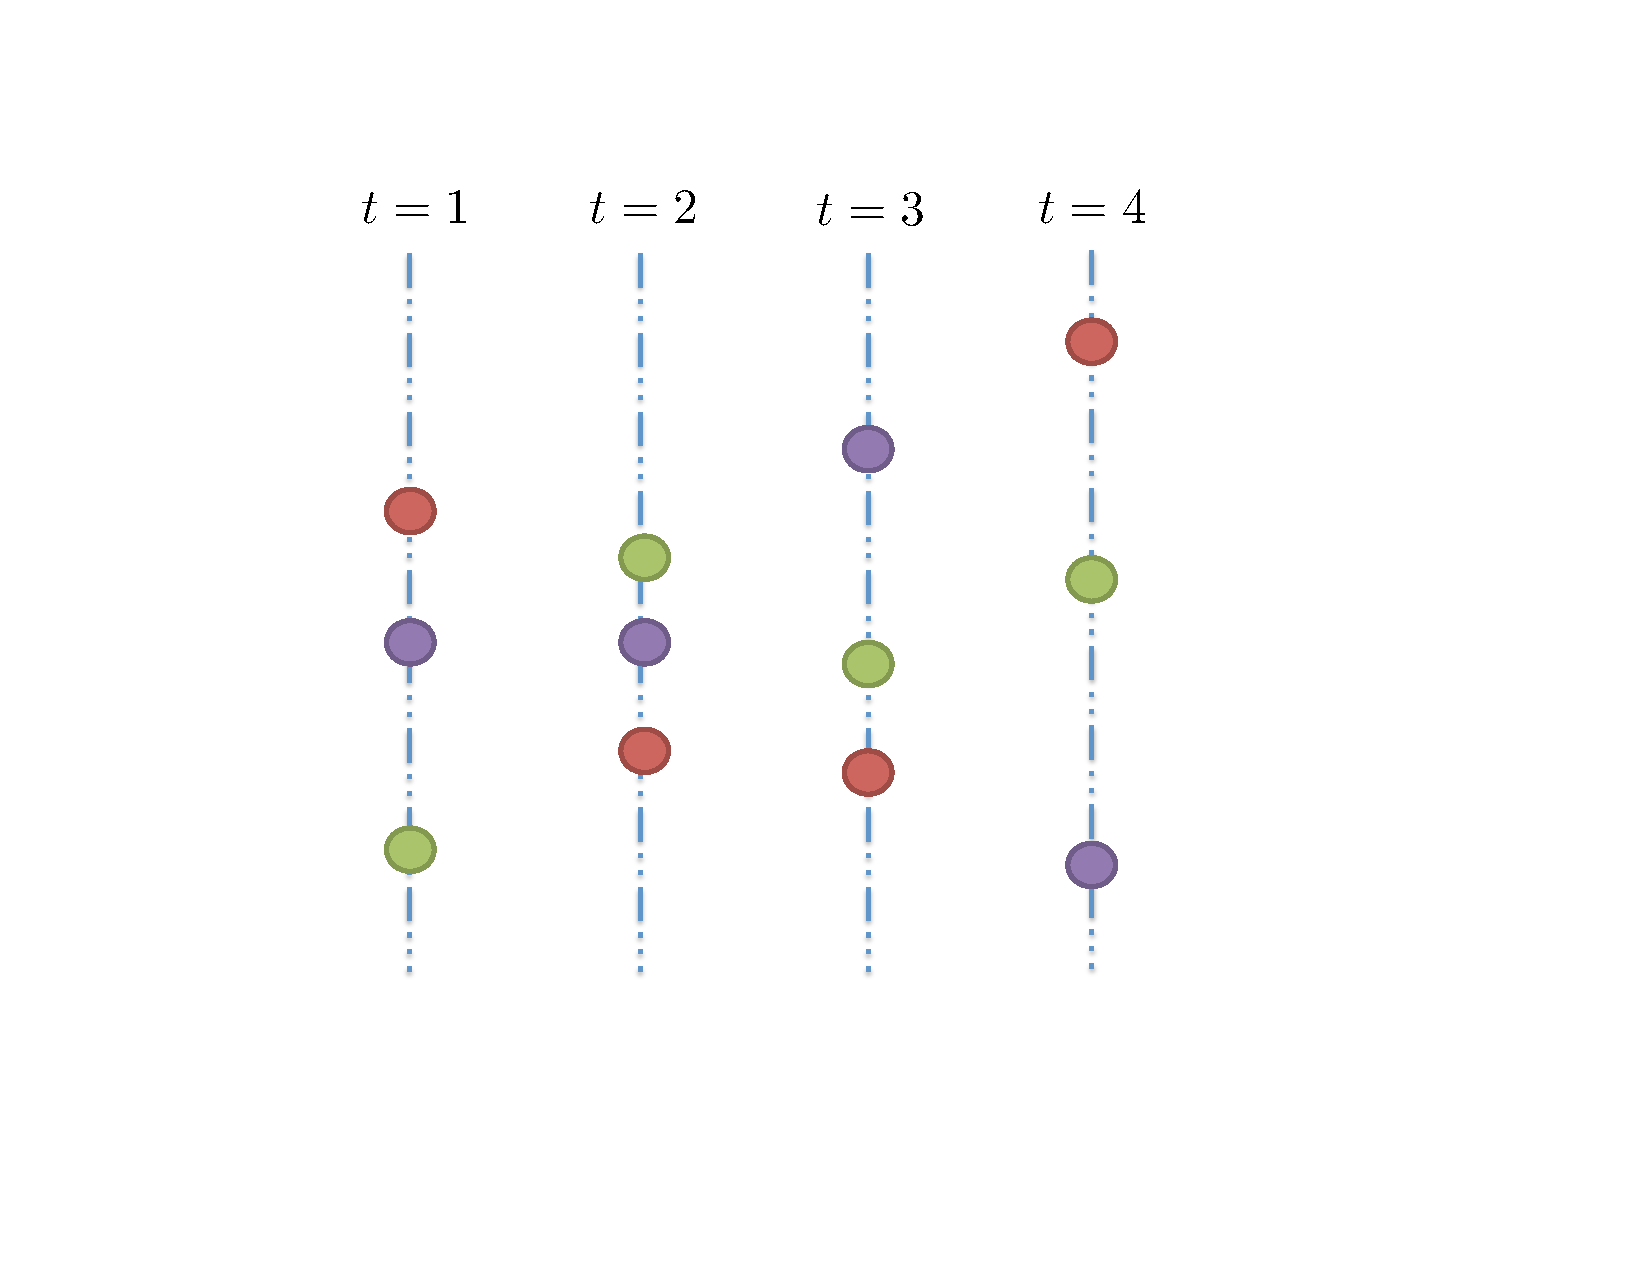
\includegraphics[ width=12cm, height=10cm,keepaspectratio]{Slide_10.pdf}
\end{frame}

\begin{frame}
\frametitle{Swapping Mechanism}
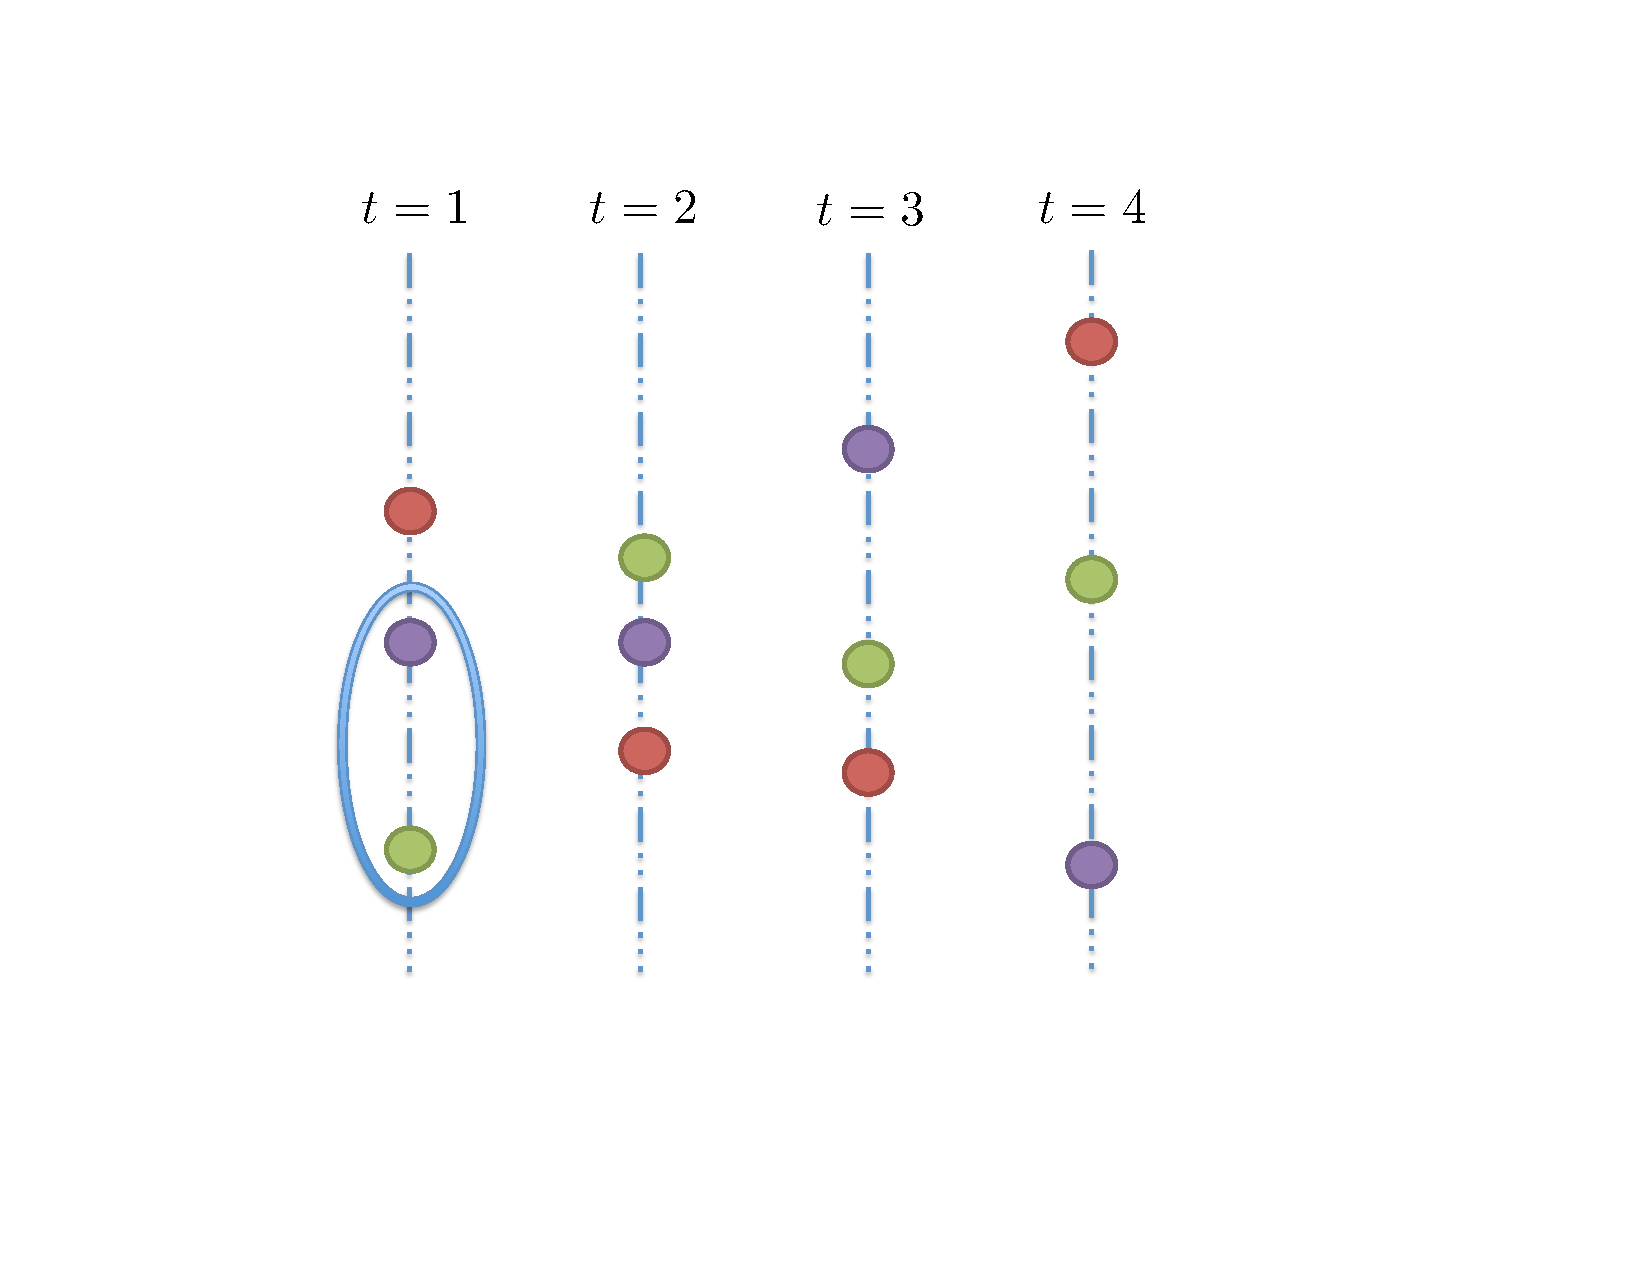
\includegraphics[ width=12cm, height=10cm,keepaspectratio]{Slide_11.pdf}
\end{frame}

\begin{frame}
\frametitle{Swapping Mechanism}
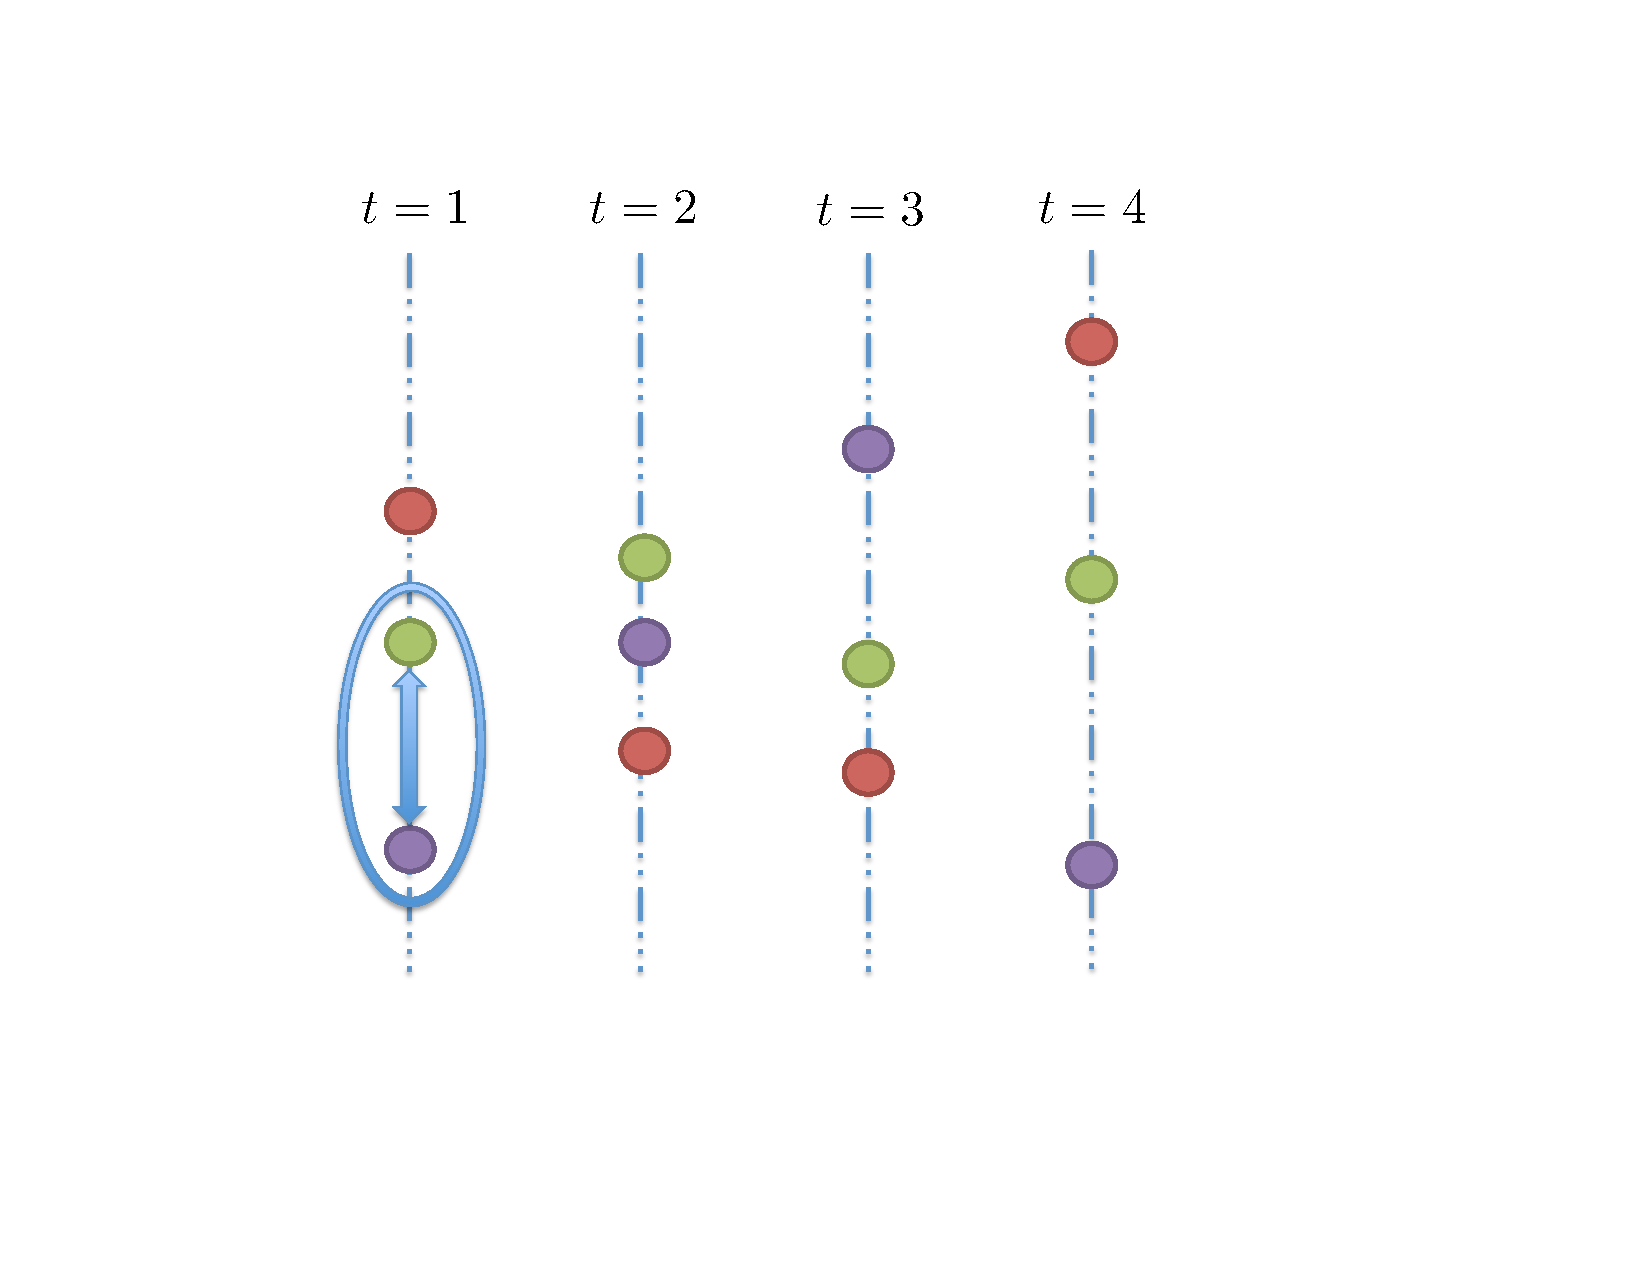
\includegraphics[ width=12cm, height=10cm,keepaspectratio]{Slide_12.pdf}
\end{frame}

\begin{frame}
\frametitle{Swapping Mechanism}
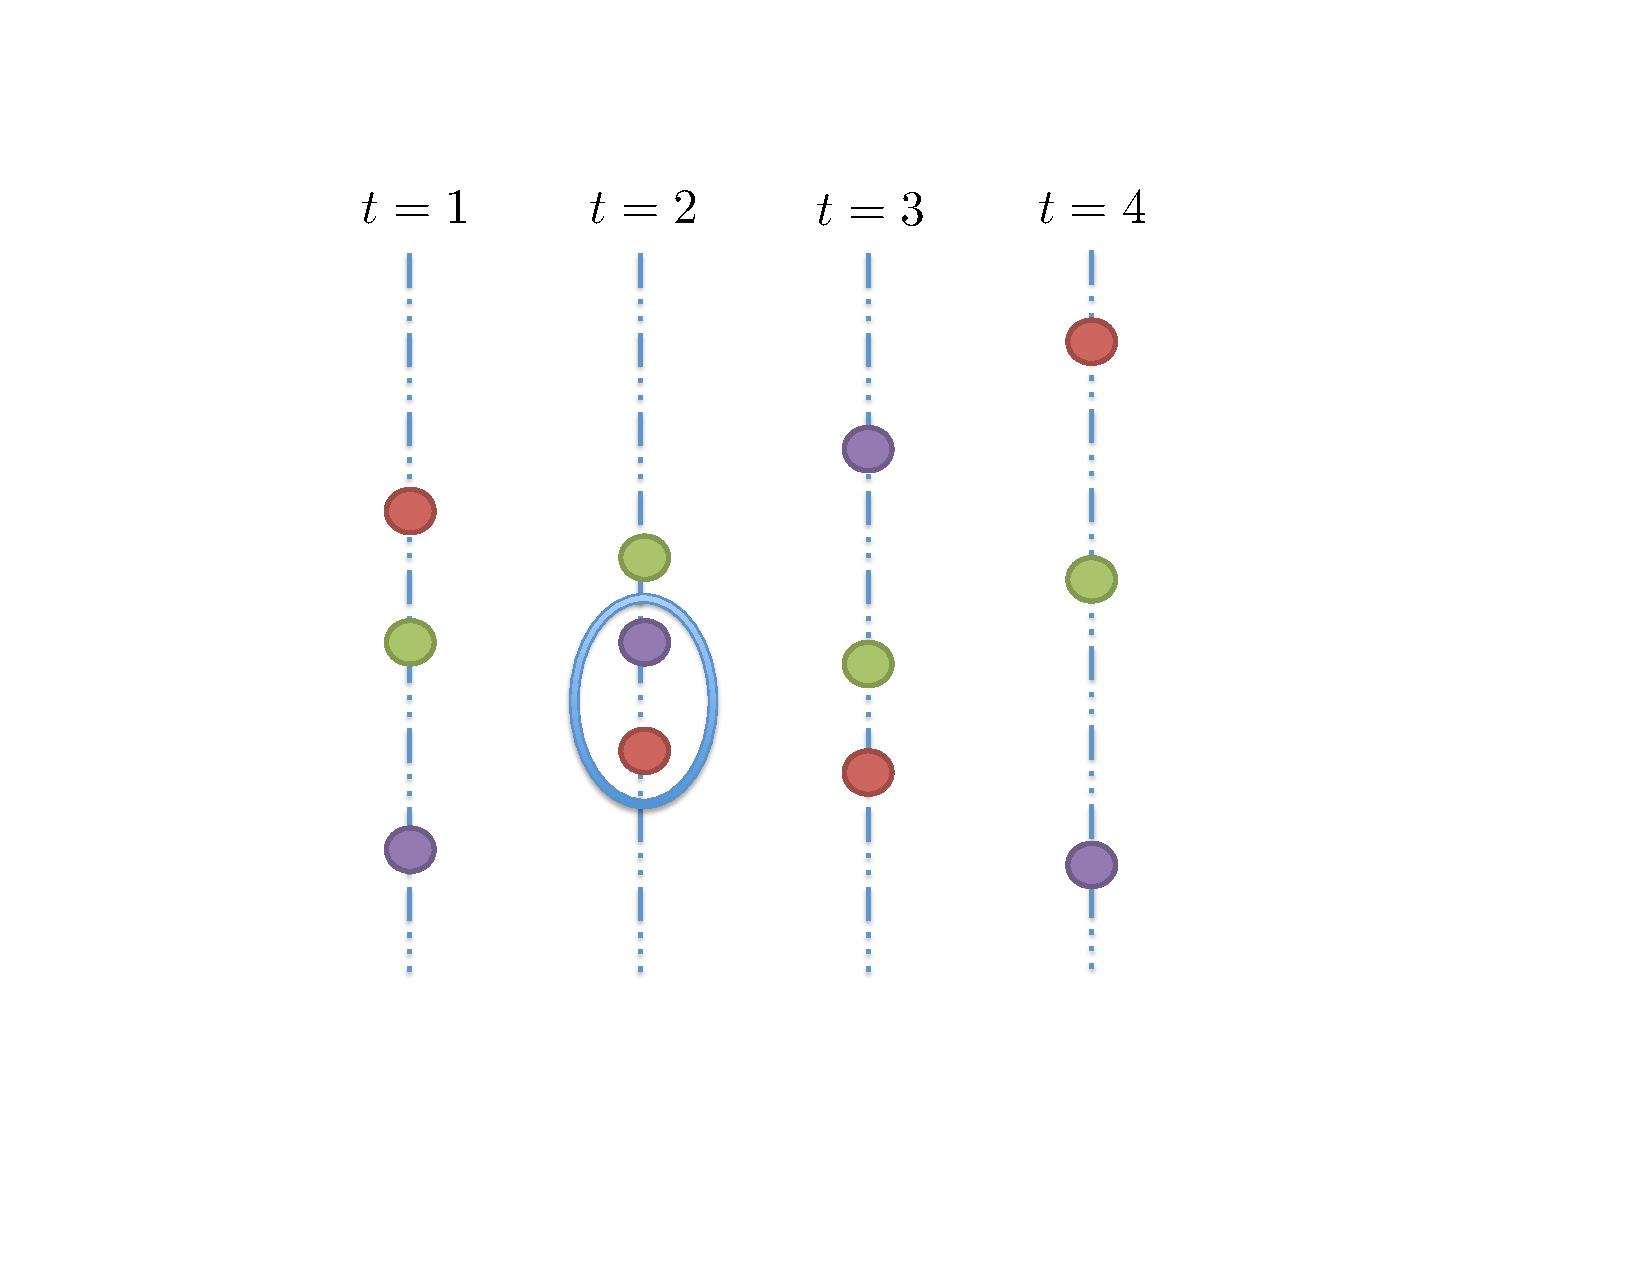
\includegraphics[ width=12cm, height=10cm,keepaspectratio]{Slide_13.pdf}
\end{frame}

\begin{frame}
\frametitle{Swapping Mechanism}
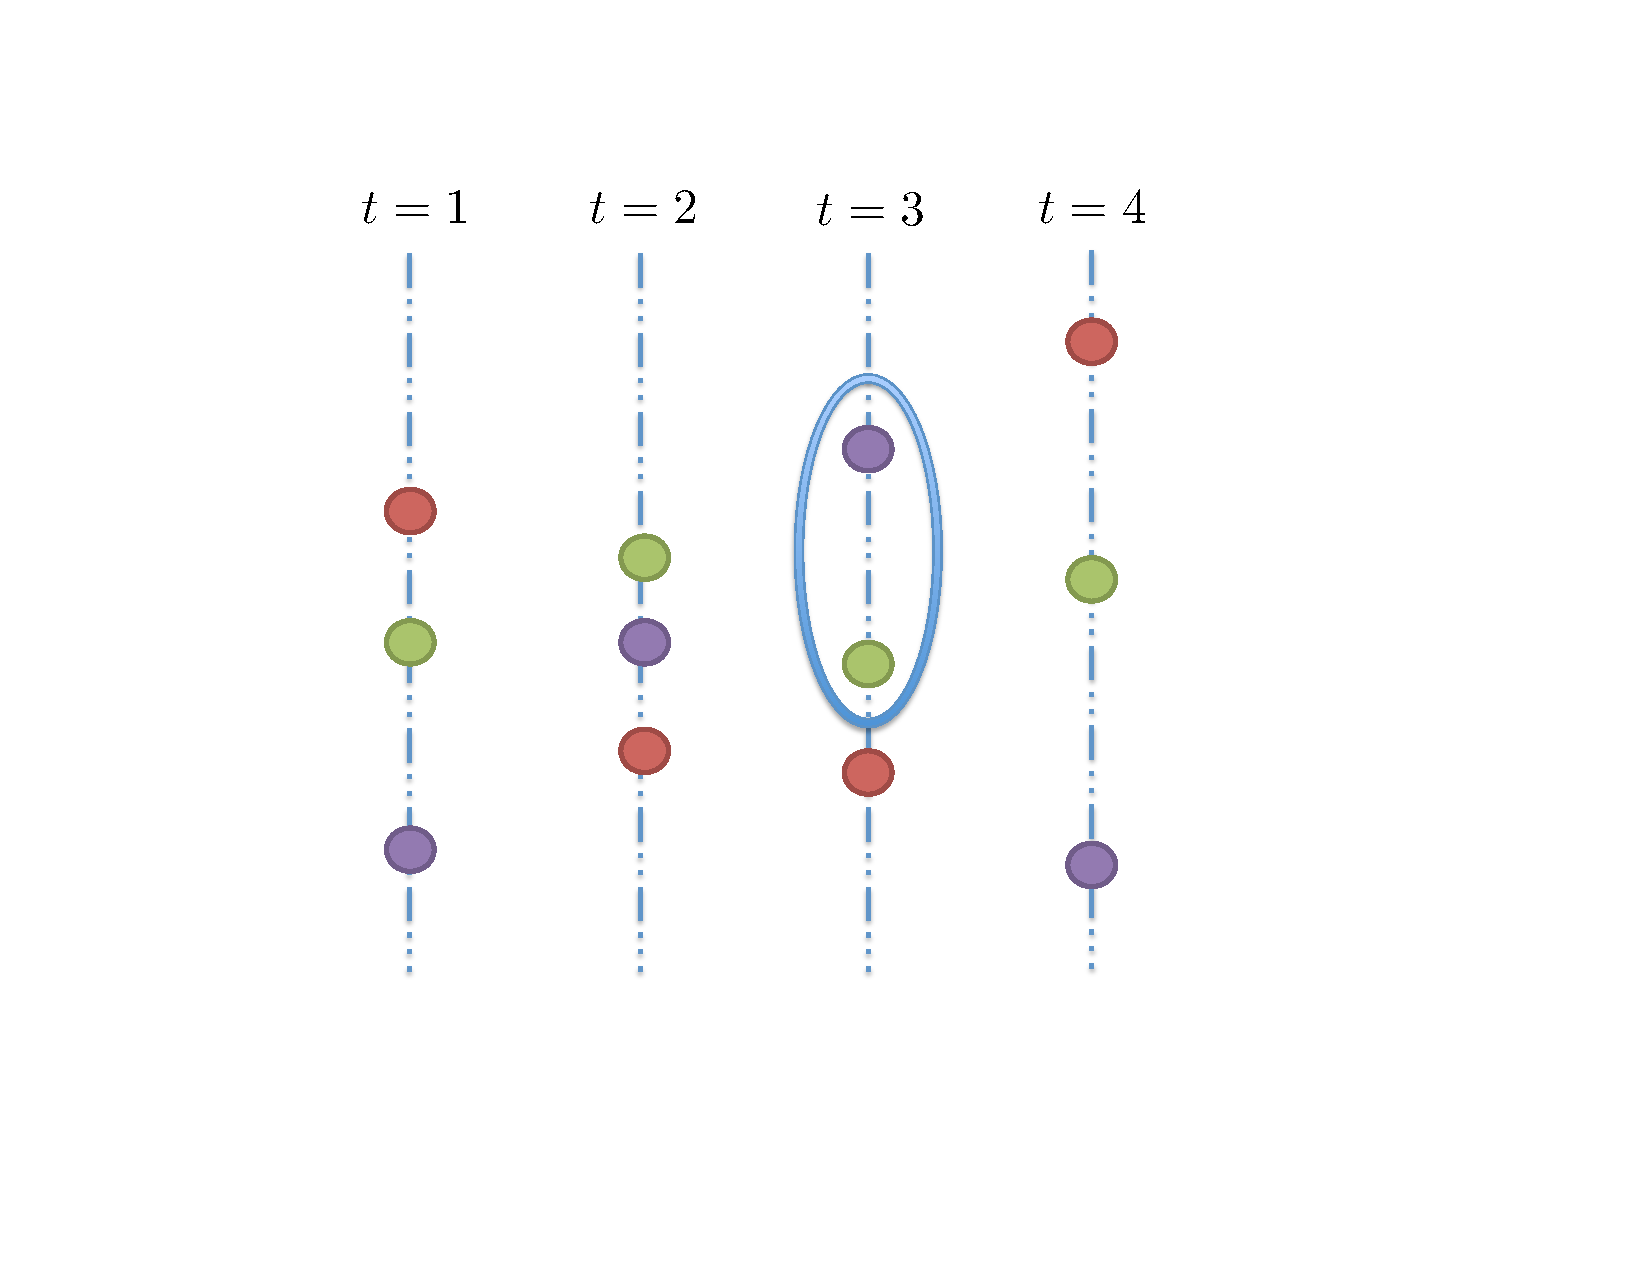
\includegraphics[ width=12cm, height=10cm,keepaspectratio]{Slide_14.pdf}
\end{frame}

\begin{frame}
\frametitle{Swapping Mechanism}
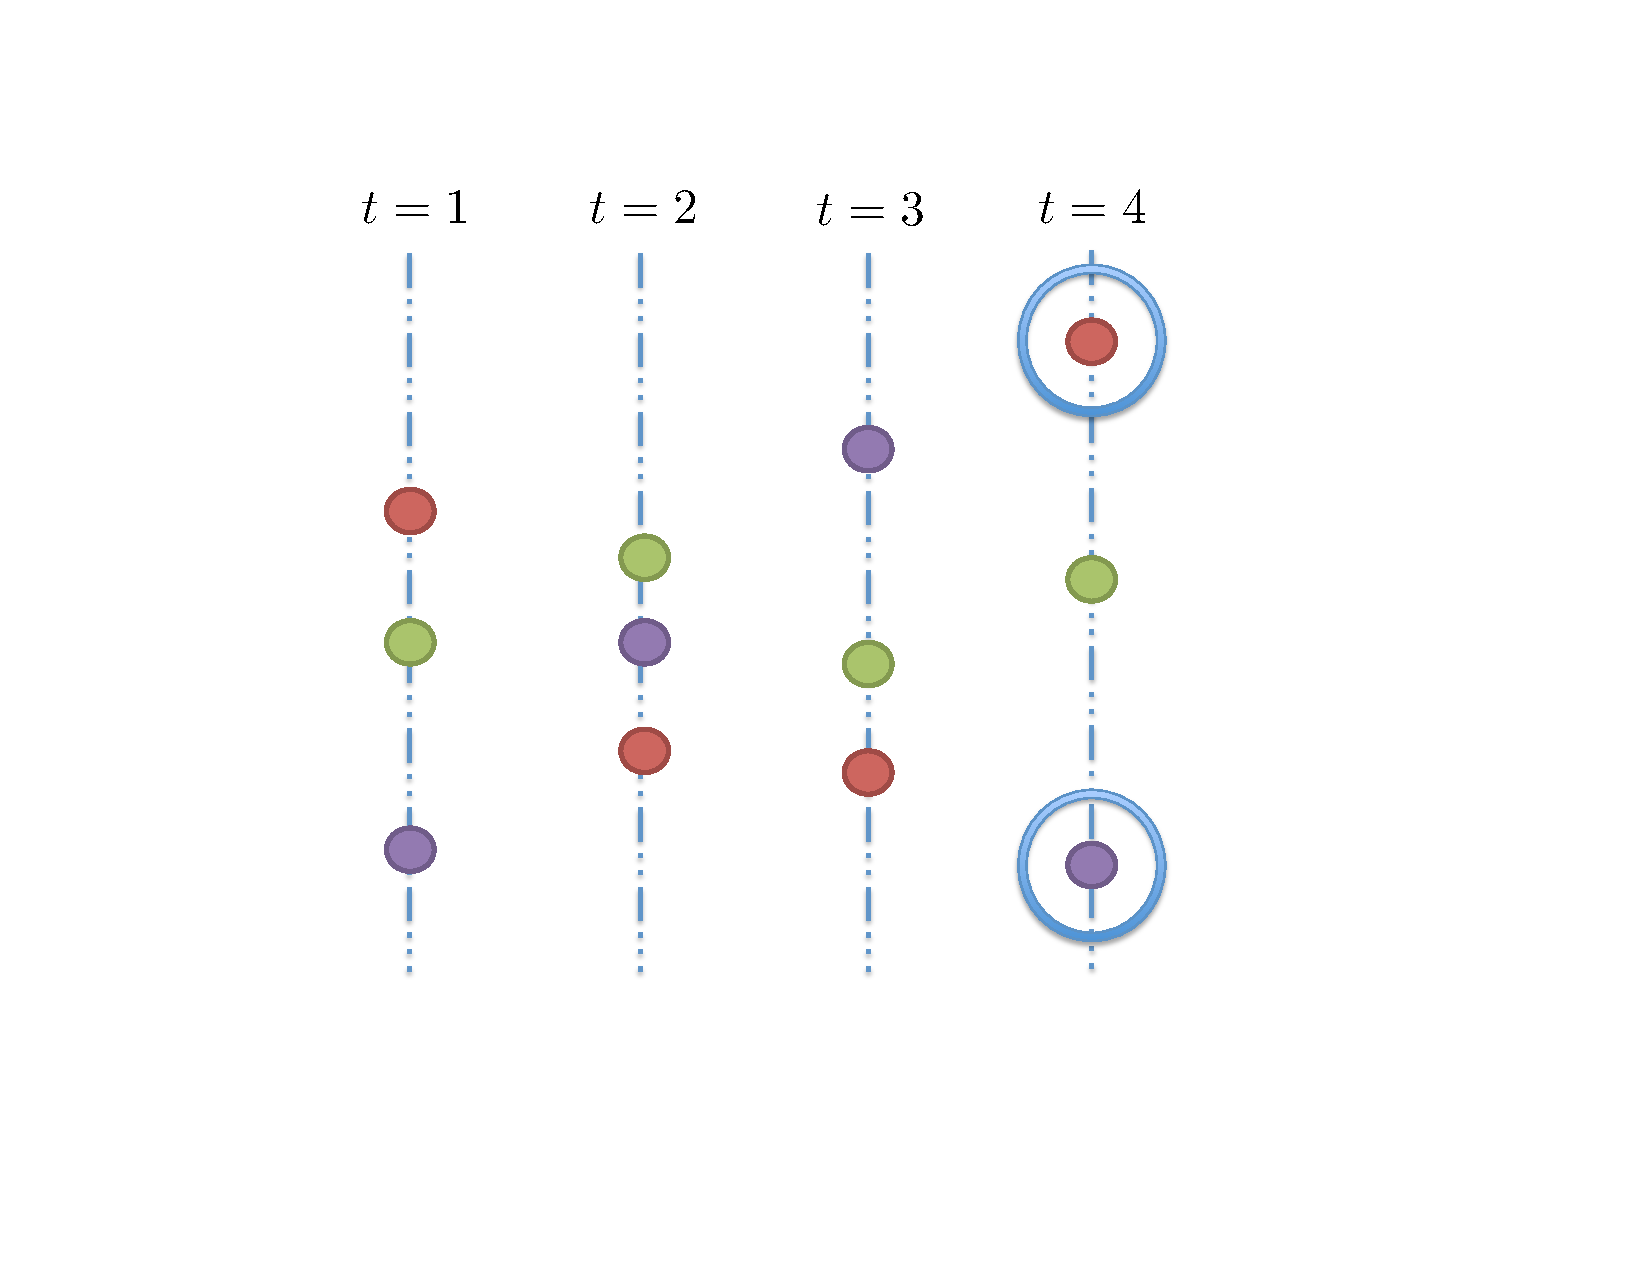
\includegraphics[ width=12cm, height=10cm,keepaspectratio]{Slide_15.pdf}
\end{frame}

\begin{frame}
\frametitle{Swapping Mechanism}
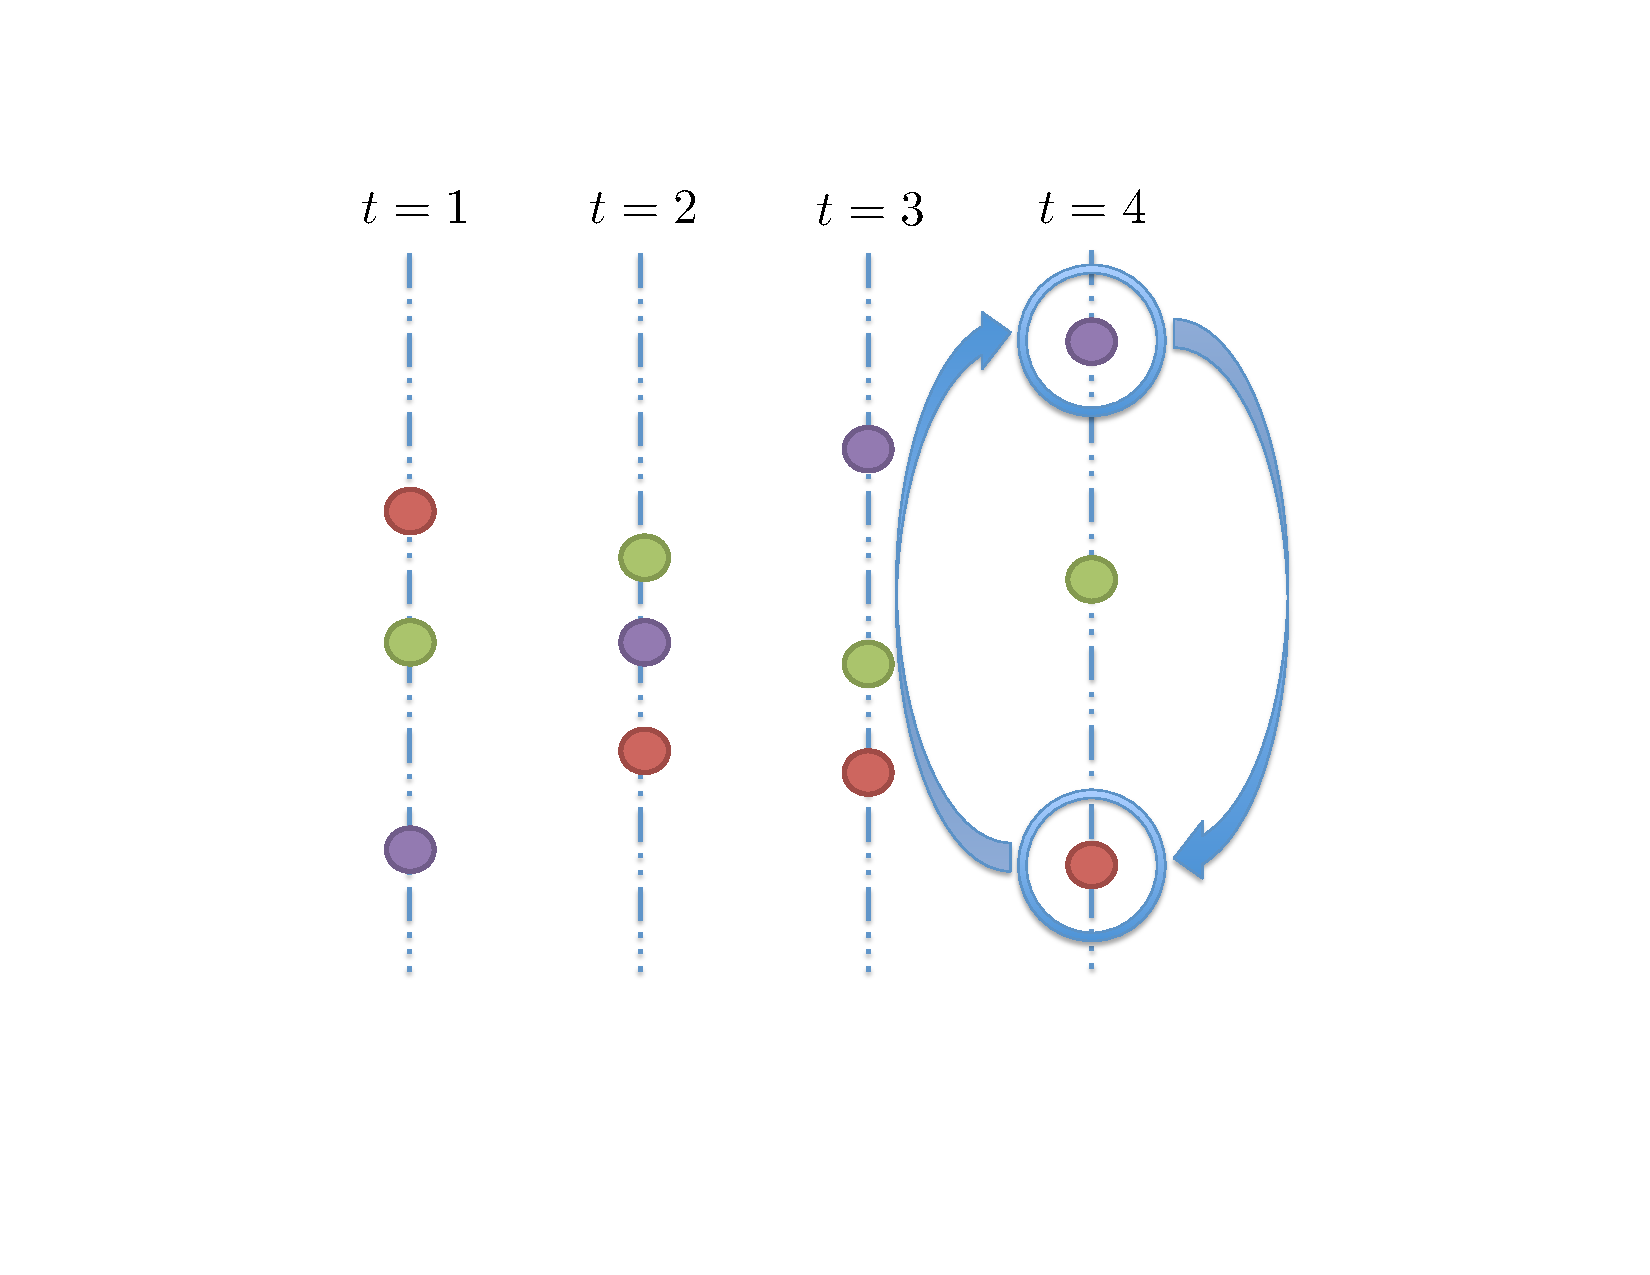
\includegraphics[ width=12cm, height=10cm,keepaspectratio]{Slide_16.pdf}
\end{frame}

\begin{frame}
\frametitle{Termination}
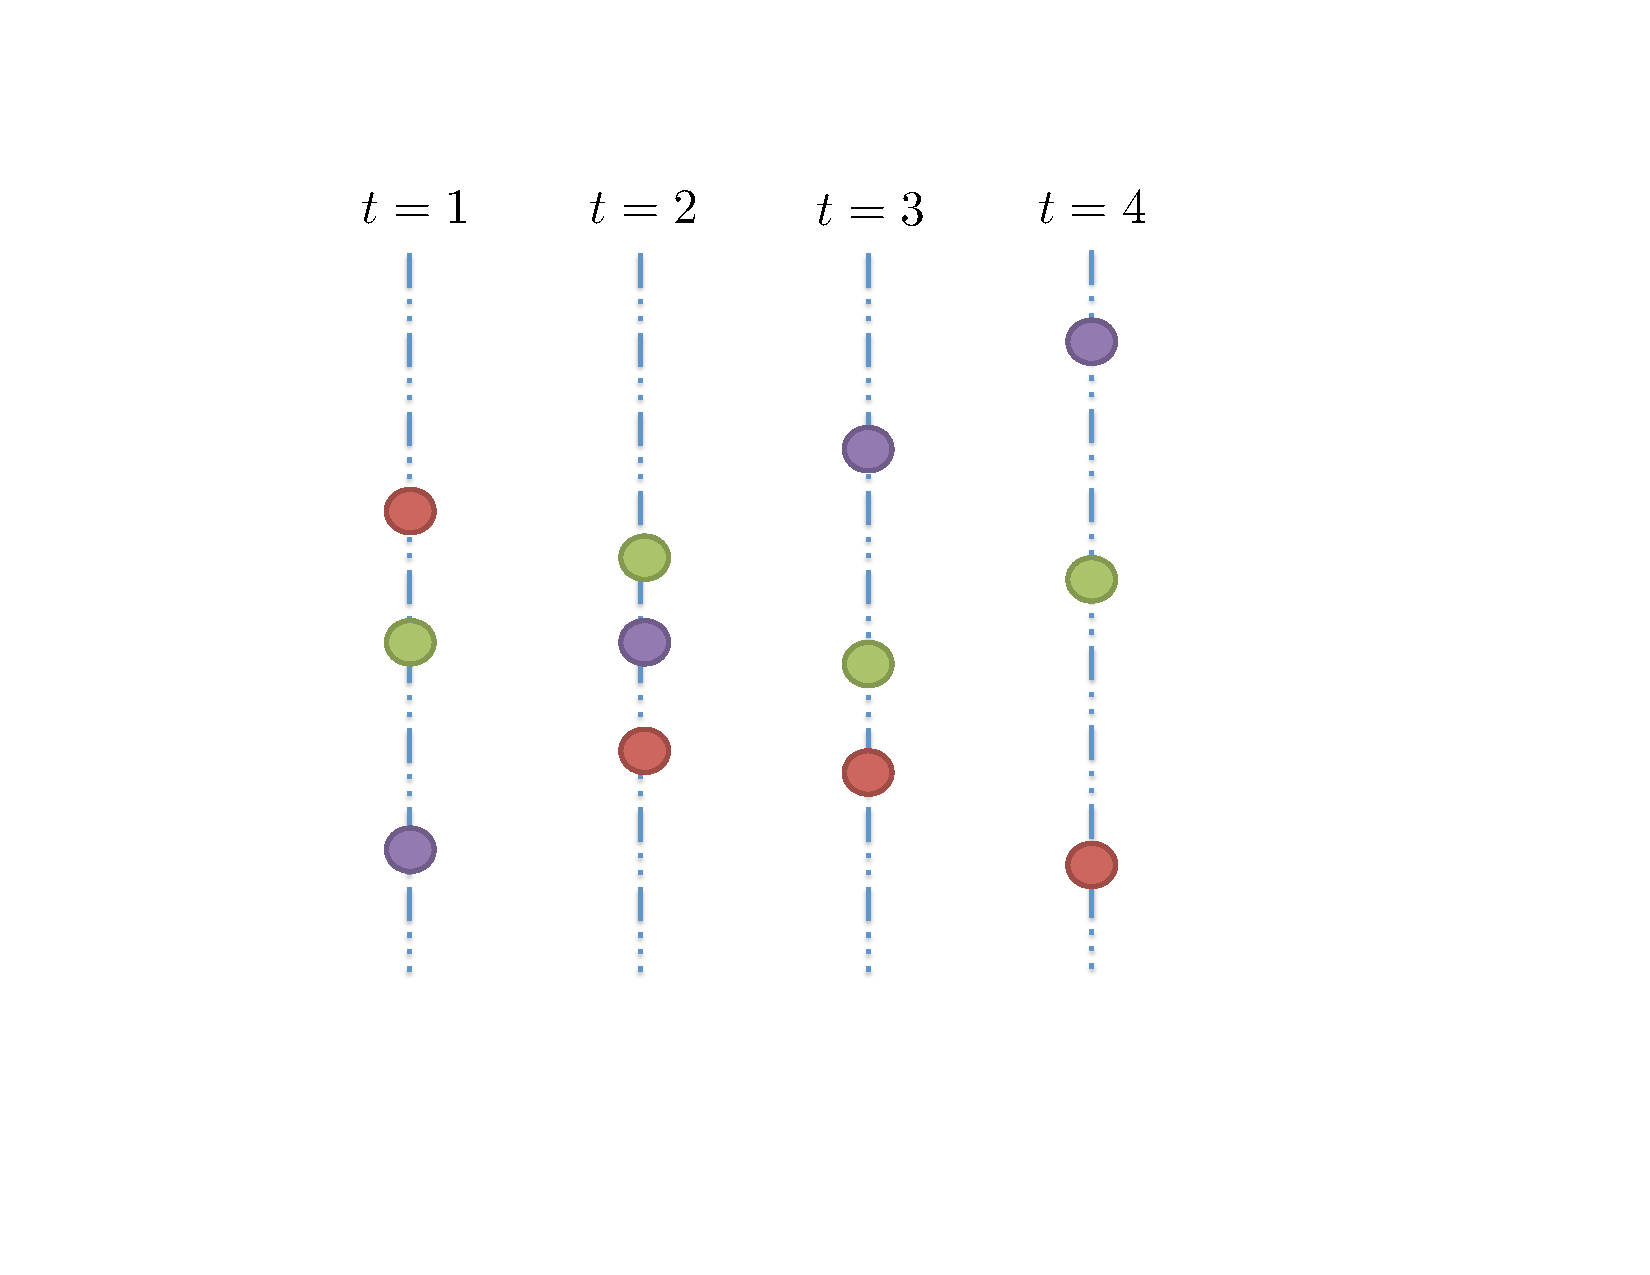
\includegraphics[ width=12cm, height=10cm,keepaspectratio]{Slide_17.pdf}
\end{frame}


%------------------------------------------------
\section{Scenario Complexity and Performance Metrics}
%------------------------------------------------

\begin{frame}
\frametitle{Data Association Complexity} 
Complexity Metric:
\begin{align*}
\rho =  \frac{\sum\limits_{t=1}^{T}\sum\limits_{i<j}c_{ijt}}{\binom{P}{2} T},
\end{align*}
where
\[c_{ijt} = 
\begin{cases}
1, & \text{if $D_{ijt} > h(\sigma)$,}\\
0, & \text{otherwise.}
\end{cases}\]
and $D_{ijt}$ is the distance between two targets $i$ and $j$ at time $t$:
\begin{align*}
D_{ijt} = \| \alpha^{\text{true}}_{i} + \beta^{\text{true}}_{i}t - \alpha^{\text{true}}_{j} + \beta^{\text{true}}_{j}t \|
\end{align*}
\end{frame}

\begin{frame}
\frametitle{Data Association Performance Metric} 
No detection ambiguity:
\begin{align*}
Accuracy =  \frac{\text{\# correct assignments}}{\text{Total \# of detections}}= \frac{\text{\# correct assignments}}{PT}
\end{align*}
Detection ambiguity:
\begin{align*}
Accuracy =  \frac{\text{\# correct assignments}}{PT + \text{\# False Alarms}}
\end{align*}
\end{frame}

\begin{frame}
\frametitle{Trajectory Estimation} 
Complexity Metric: $\sigma$
\newline
Performance Metric:
\begin{align*}
	\delta = \frac{\sum\limits_{t=1}^{T}\sum\limits_{j=1}^{P}\| \bar{x}_{jt} - \hat{x}_{jt} \|}{PT}
\end{align*}
where:
\begin{align*}
	\bar{x}_{jt} = \alpha^{\text{true}}_{j} + \beta^{\text{true}}_{j}t.
\end{align*}
\begin{align*}
	\hat{x}_{jt} =  \alpha_{j} + \beta_{j}t.
\end{align*}
\end{frame}

%------------------------------------------------
\section{Experimental Simulations and Computational Results}
%------------------------------------------------

\begin{frame}
\frametitle{Sigma vs.Rho} 
\begin{figure}[ht]
  \centering
  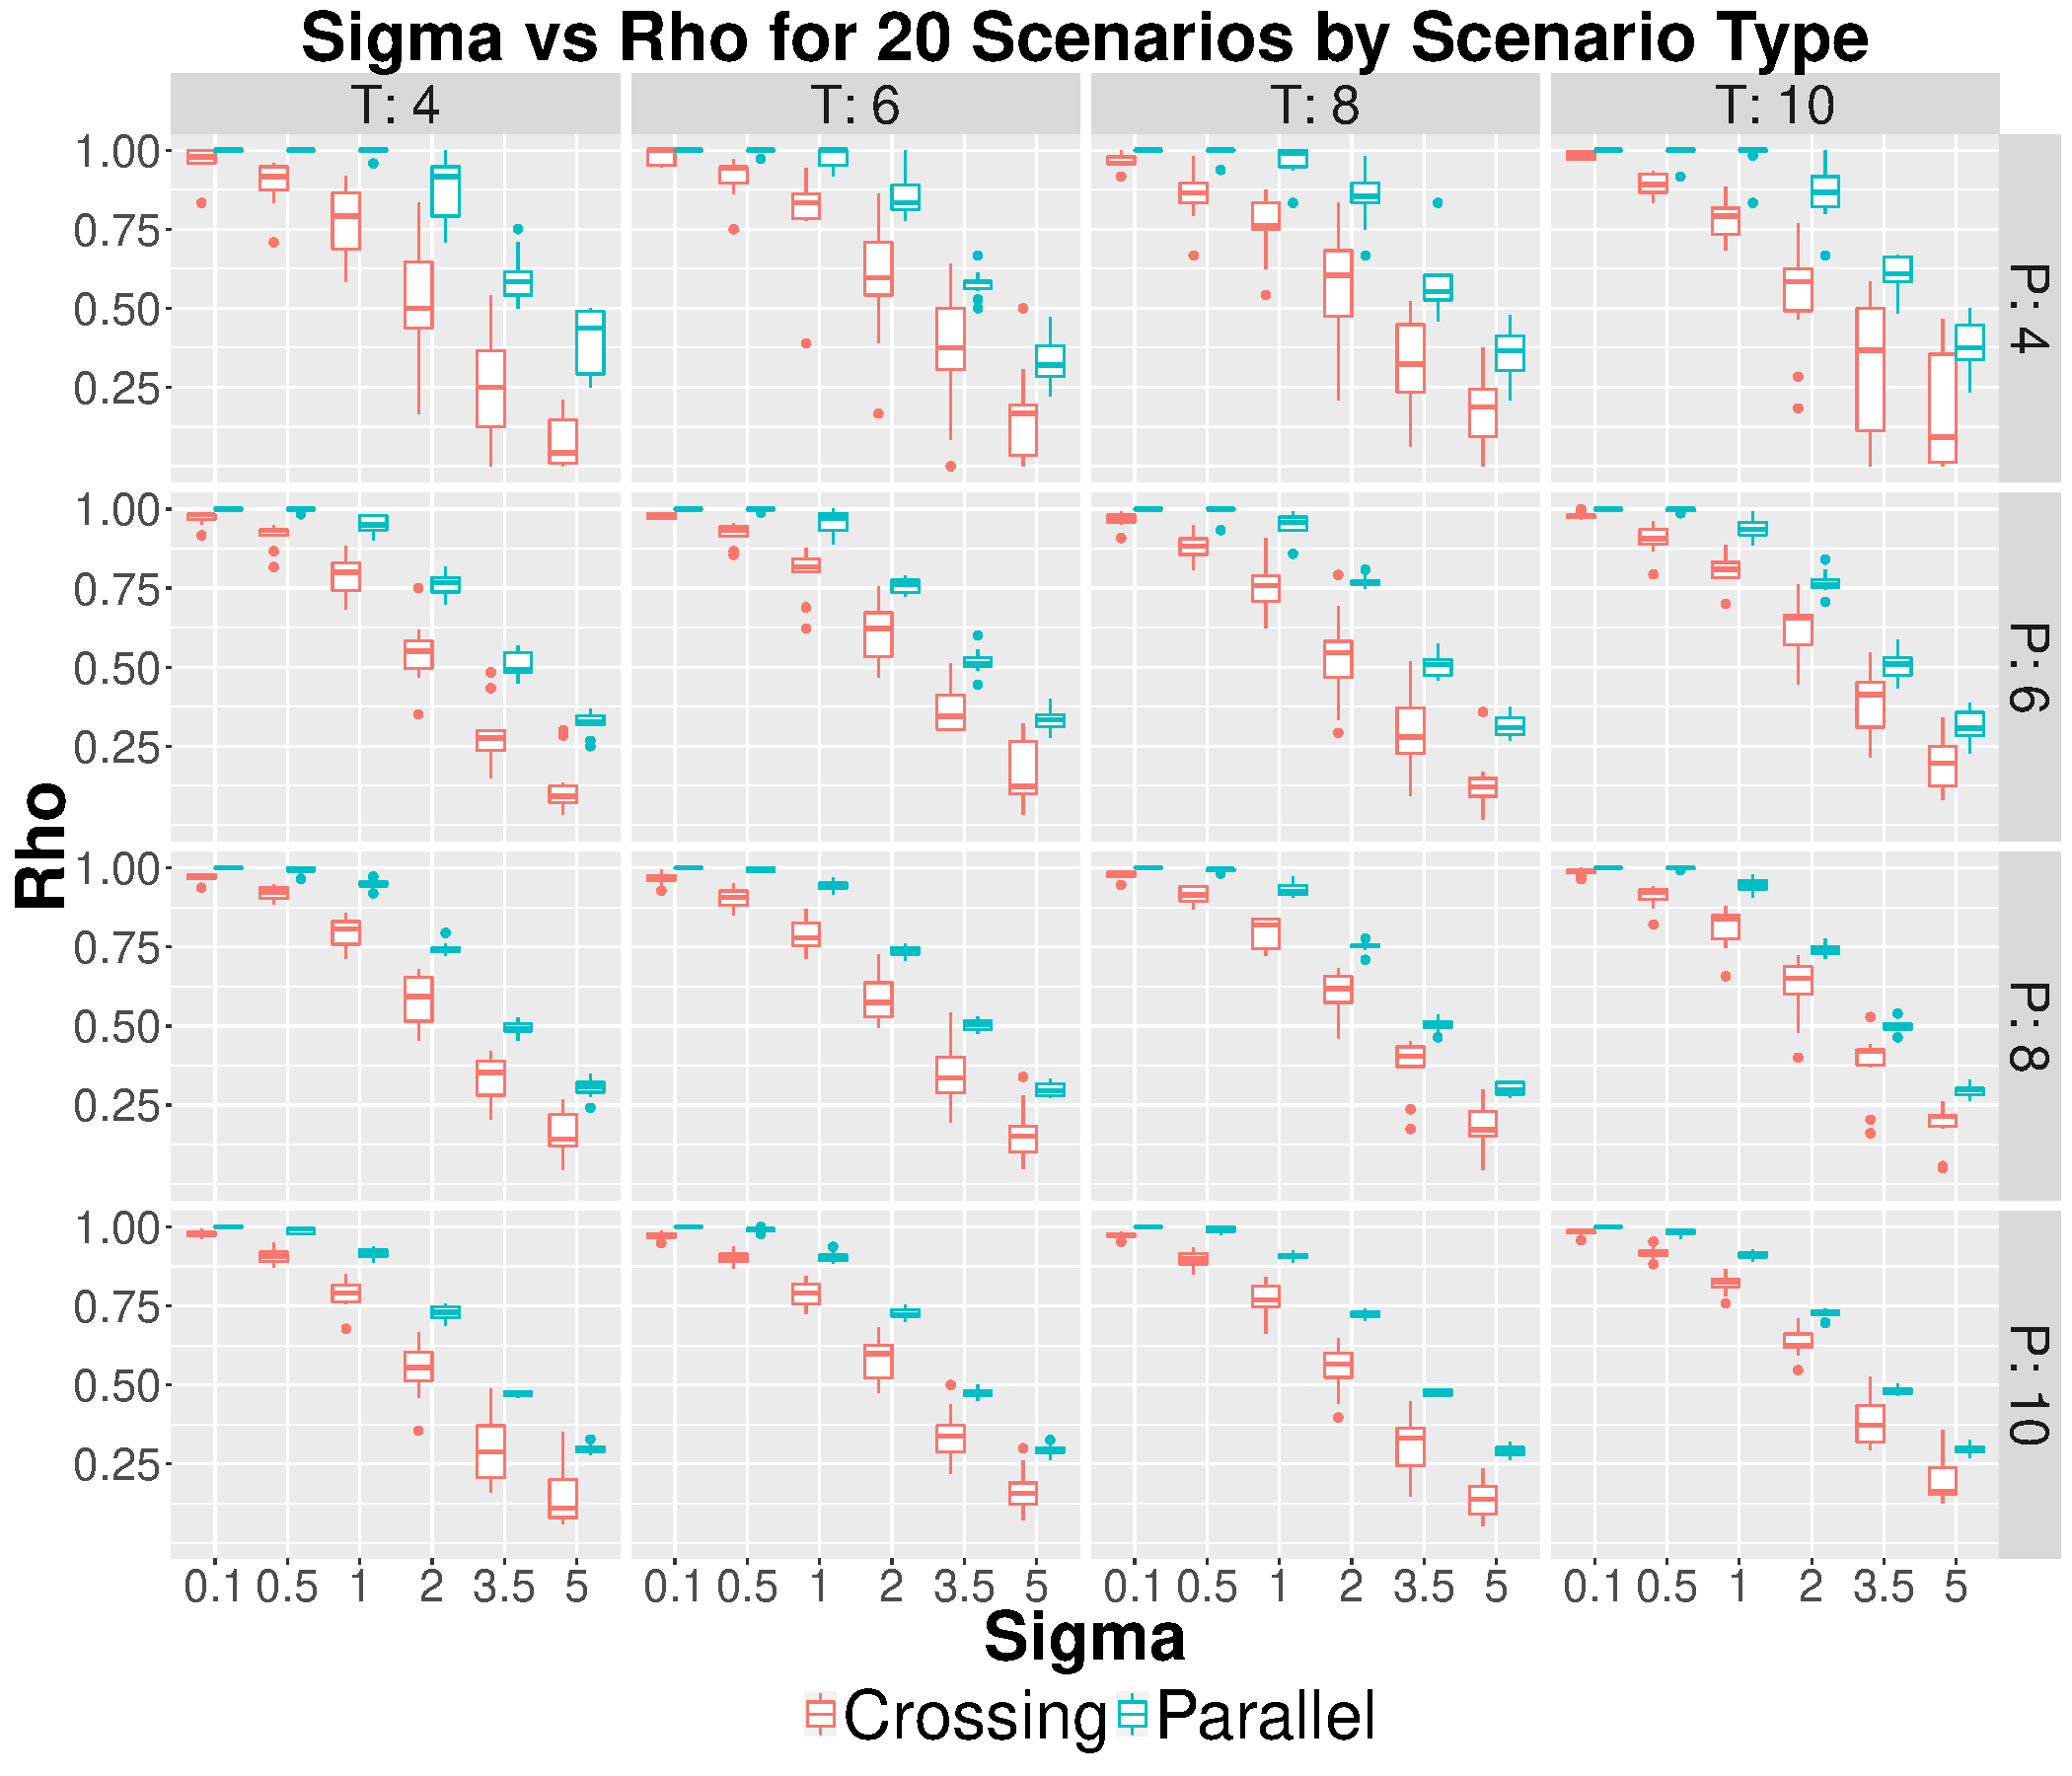
\includegraphics[width=.7\columnwidth]{../Figures//Sigma_vs_Rho}
    \caption{Relationship between $\sigma$ and $\rho$ summarized by scenario type for all 20 generated scenarios in this experiment.}
    \label{fig:Sigma_vs_Rho}
\end{figure}
\end{frame}


\begin{frame}
\frametitle{Heuristic Run Times}
\begin{table}\tiny
\centering
\begin{tabular}{cc|ccc}
  \hline
   & & \multicolumn{3}{c}{Basic Heuristic Run Times } \\
   & & \multicolumn{3}{c}{(in milliseconds)}\\
   P & T & $\;\;$Min$\:\;$ & Mean & Max \\ 
  \hline
  \hline
   4 & 4 & 0.07 & 0.10 & 0.18 \\ 
   4 & 6 & 0.18 & 0.24 & 0.38 \\ 
   4 & 8 & 0.34 & 0.45 & 0.62 \\ 
   4 & 10 & 0.58 & 0.76 & 1.02 \\ 
   6 & 4 & 0.11 & 0.15 & 0.25 \\ 
   6 & 6 & 0.31 & 0.39 & 0.58 \\ 
   6 & 8 & 0.64 & 0.81 & 1.05 \\ 
   6 & 10 & 1.24 & 1.56 & 2.02 \\ 
   8 & 4 & 0.14 & 0.19 & 0.30 \\ 
   8 & 6 & 0.46 & 0.57 & 0.86 \\ 
   8 & 8 & 0.95 & 1.24 & 1.58 \\ 
   8 & 10 & 2.07 & 2.53 & 3.37 \\ 
   10 & 4 & 0.19 & 0.25 & 0.41 \\ 
   10 & 6 & 0.63 & 0.80 & 1.03 \\ 
   10 & 8 & 1.44 & 1.84 & 2.44 \\ 
   10 & 10 & 2.96 & 3.73 & 4.56 \\ 
   \hline
\end{tabular}
\end{table}
\end{frame}

\begin{frame}
\frametitle{Solution Types}
Two Benchmark Solutions:
\begin{enumerate}
\item \textit{Random} := randomly generate detection assignments
\item \textit{Ideal} := detection assignments are exactly correct
\end{enumerate}\vfill
Two Algorithmic Solutions:
\begin{enumerate}
\item \textit{Heuristic} := initialized with 1,000 starting points
\item \textit{MIO Model} := heuristic solution provided as a warm start
\end{enumerate}
\end{frame}

\begin{frame}
\frametitle{Data Association Accuracy}
\begin{figure}[ht]
  \centering
  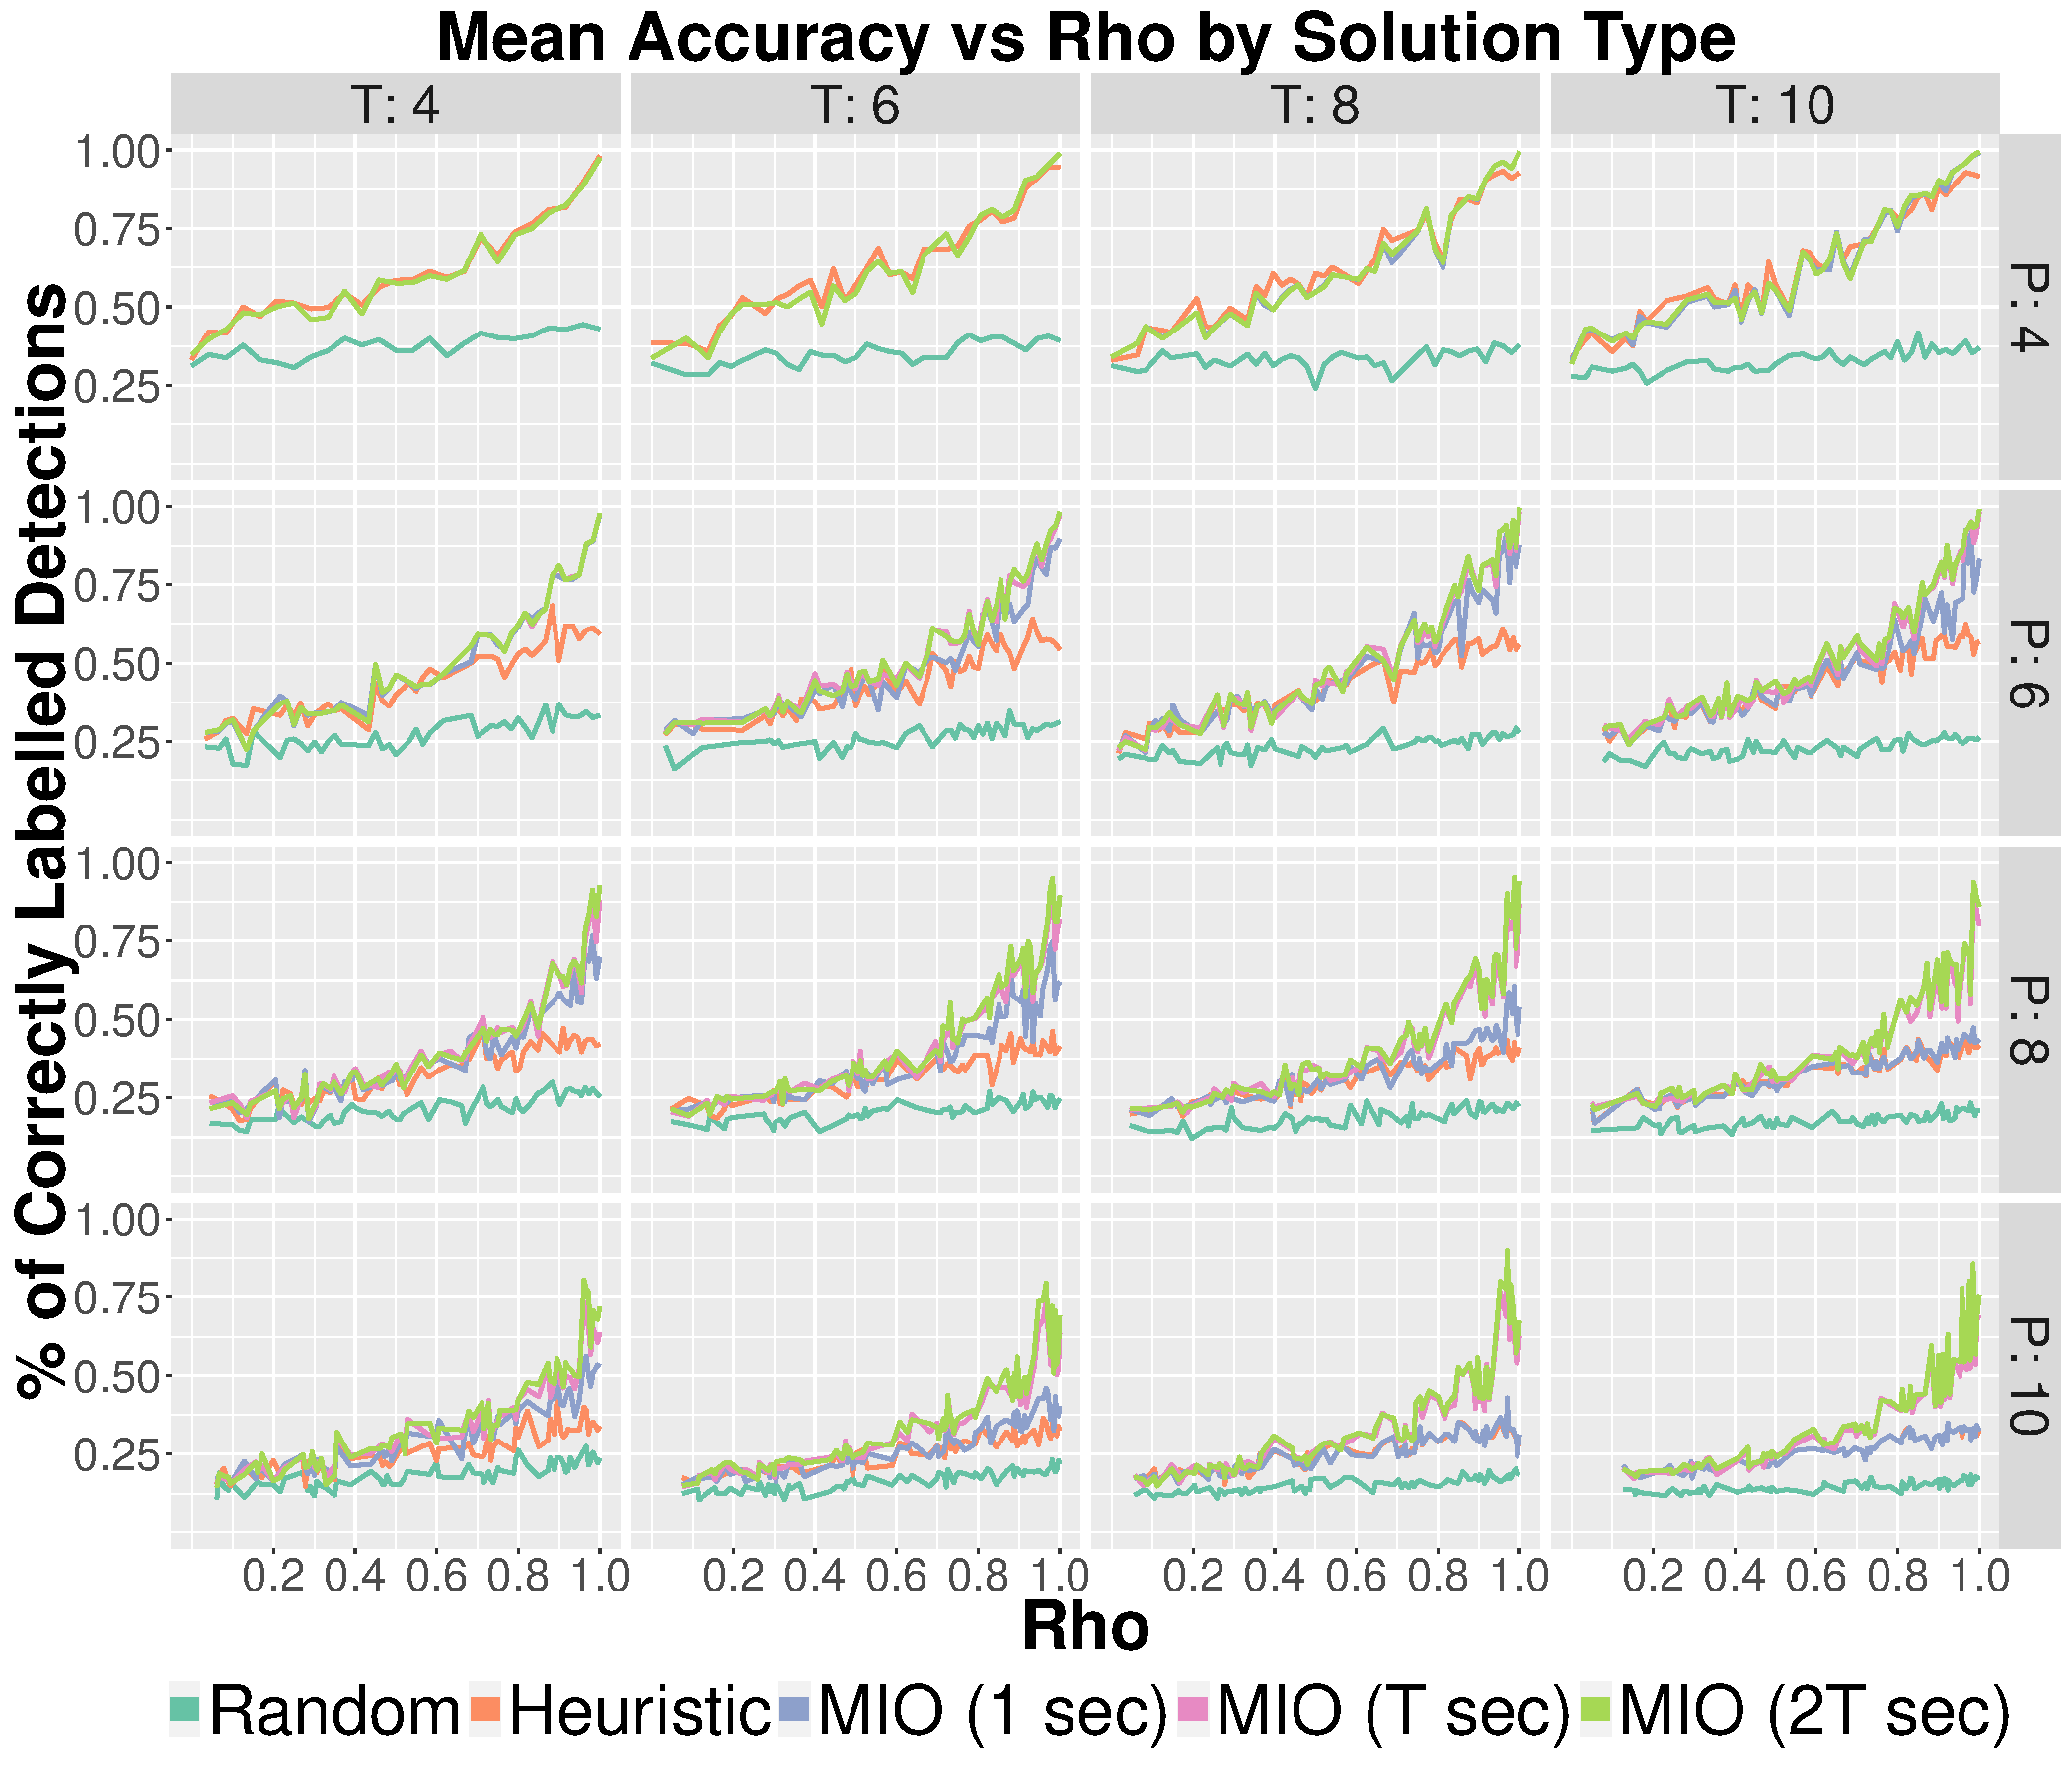
\includegraphics[width=.7\columnwidth]{../Figures/Basic_Accuracy_Summary}
\end{figure}
\end{frame}

\begin{frame}
\frametitle{Trajectory Estimation Error} 
\begin{figure}[ht]
  \centering
  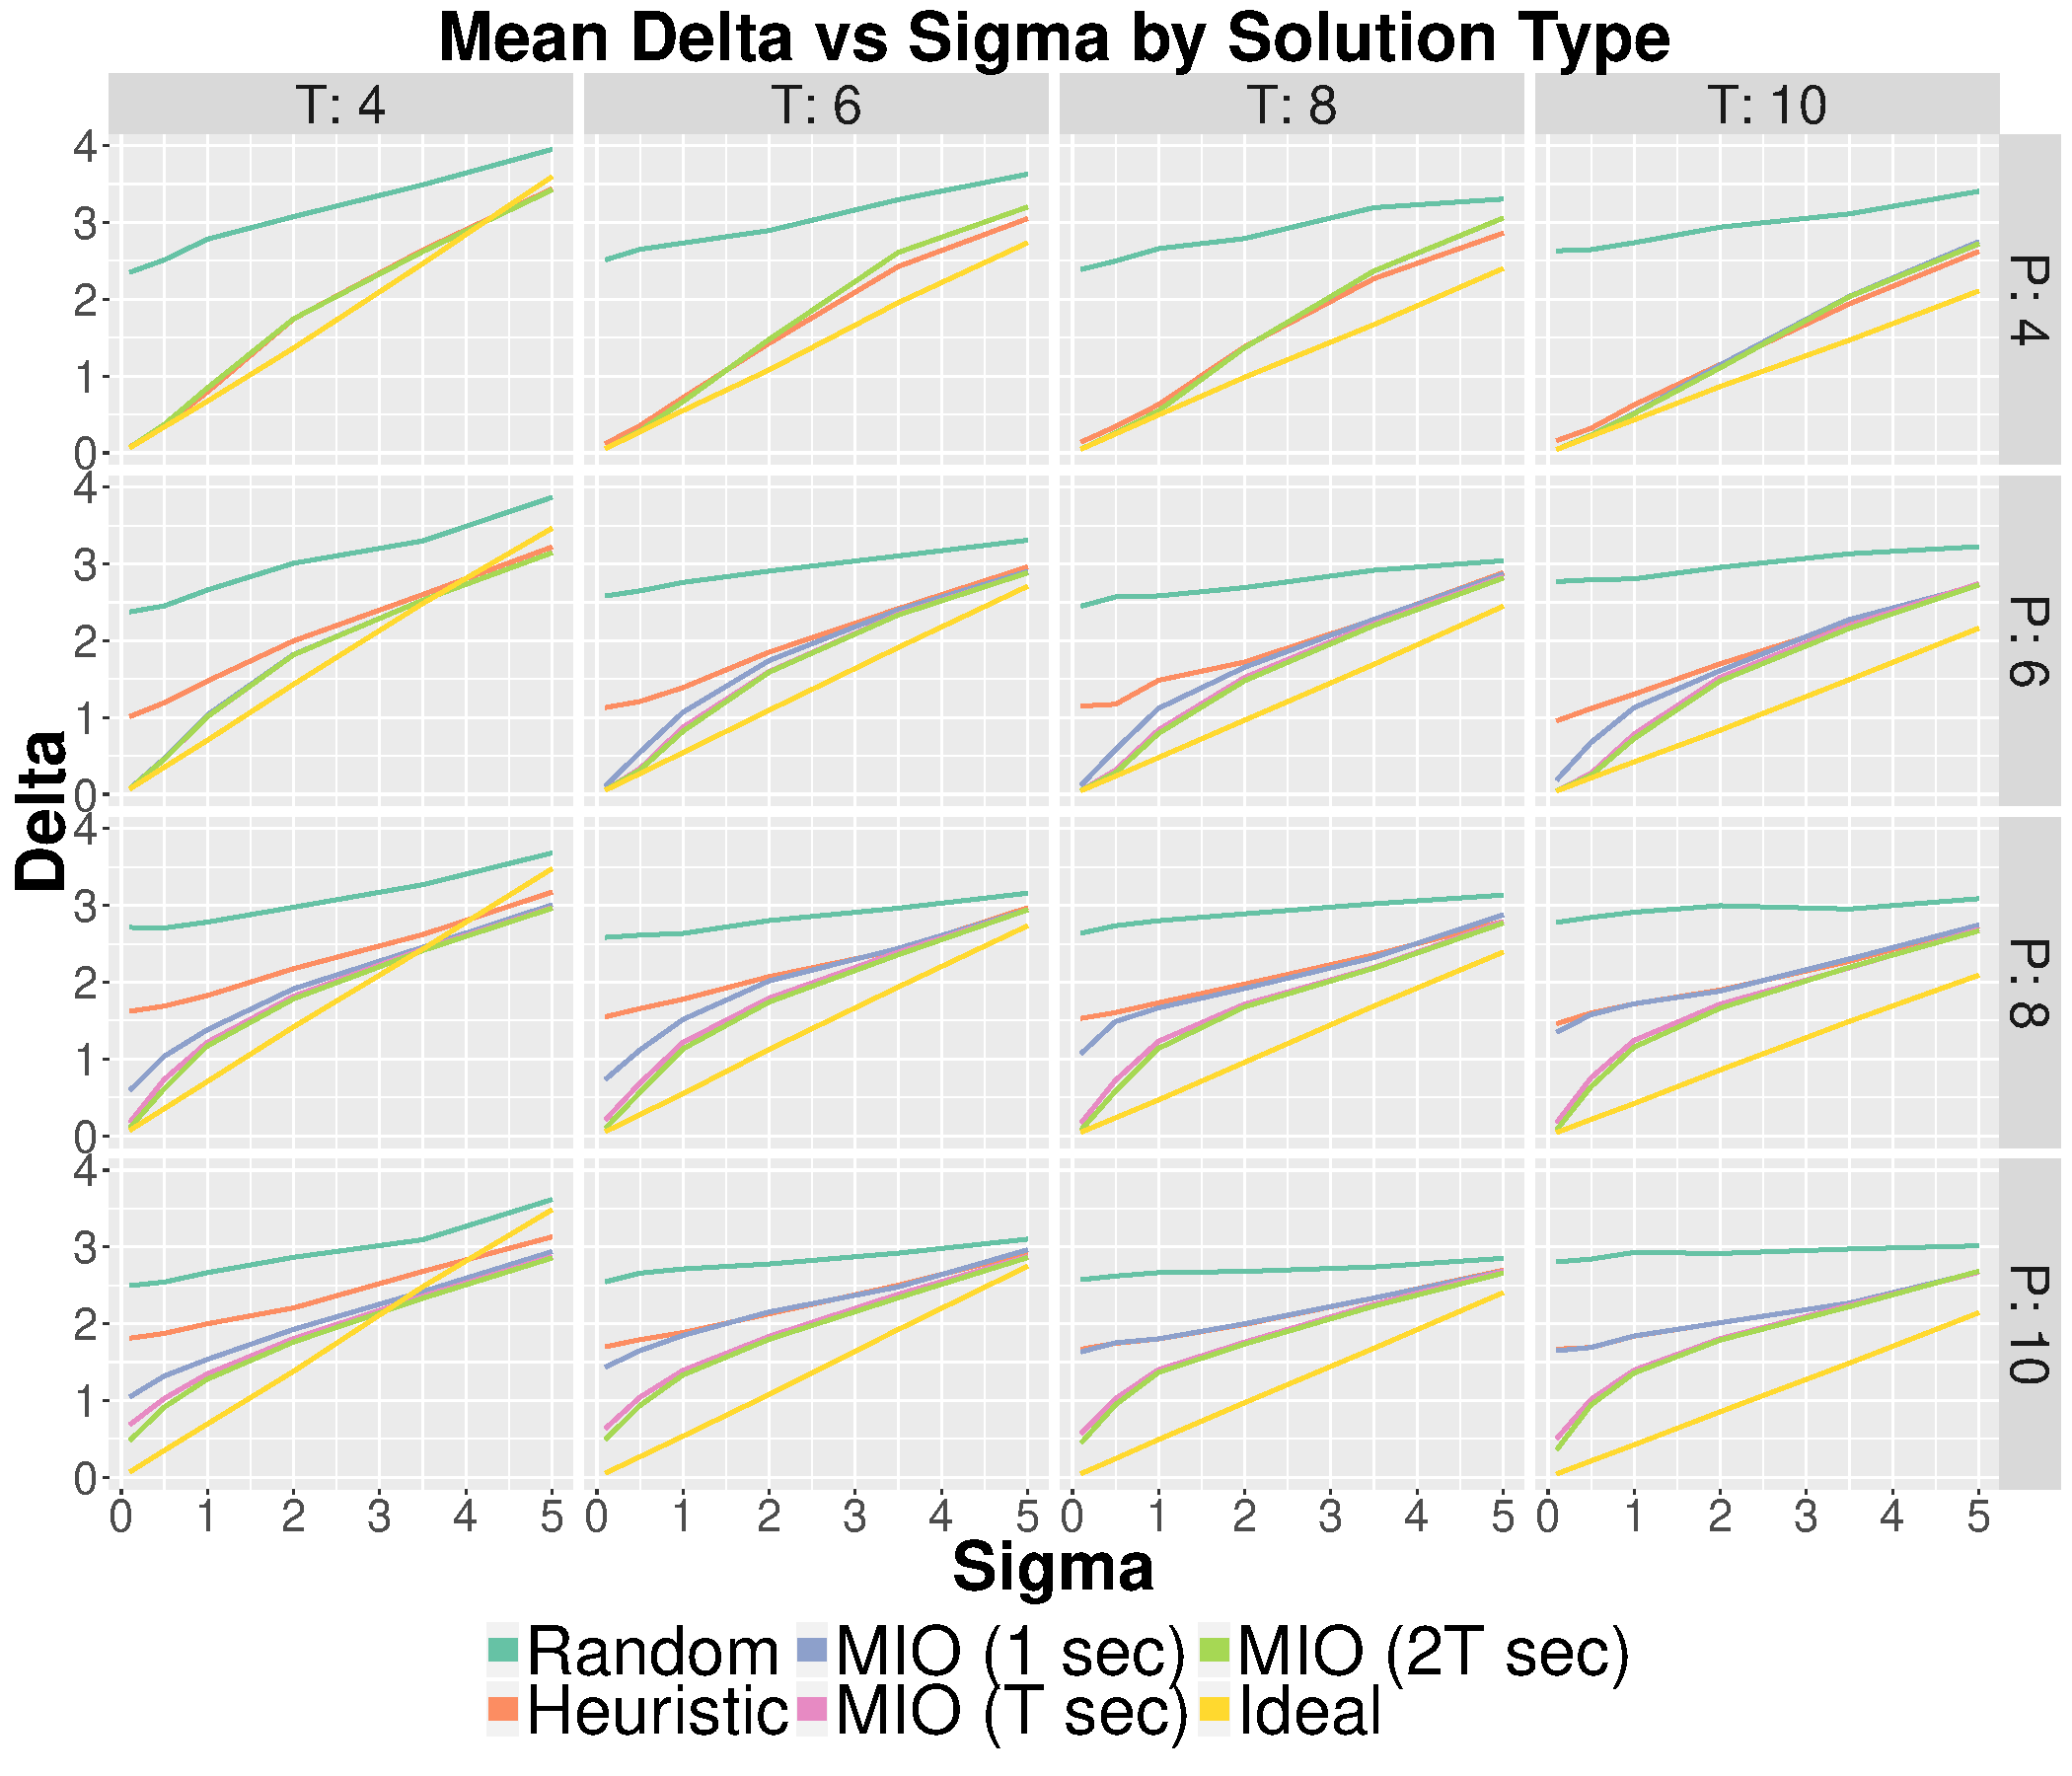
\includegraphics[width=.7\columnwidth]{../Figures/Basic_Delta_Summary}
\end{figure}
\end{frame}

\begin{frame}
\frametitle{Summary of cases without detection ambiguity} 
\begin{itemize}
\item Heuristic
\begin{itemize}
\item Runs in milliseconds for single starting point
\item Scalability maintained through parallelization
\end{itemize}
\item MIO
\begin{itemize}
\item Scalable with respect to increases in both $P$ and $T$
\item Warm start crucial for scalability
\item High quality solutions after $T$ or fewer seconds. 
\item Tradeoff between correct data associations good trajectory estimation
\item Increasing $T$ $\Rightarrow$ improved solution quality\\
$\qquad \qquad \quad \; \; \Rightarrow$ increased computational complexity\\
\end{itemize}
\end{itemize}
\end{frame}

\begin{frame}
\frametitle{Robust Heuristic Run Times}
\begin{table}\tiny
\centering
\begin{tabular}{cc|ccc}
  \hline
   & & \multicolumn{3}{c}{Robust Heuristic Run Times} \\
   & & \multicolumn{3}{c}{(in milliseconds)}\\
   $ P_{\text{estimated}}$ & T & $\;\;$Min$\;\;$ & Mean & Max \\ 
  \hline
  \hline
  2 & 4 & 0.15 & 0.23 & 0.41 \\ 
  2 & 6 & 0.42 & 0.56 & 0.93 \\ 
  2 & 8 & 0.77 & 1.04 & 2.24 \\ 
  2 & 10 & 1.27 & 1.73 & 3.07 \\ 
  4 & 4 & 0.15 & 0.34 & 1.04 \\ 
  4 & 6 & 0.50 & 0.94 & 2.69 \\ 
  4 & 8 & 1.09 & 1.88 & 3.87 \\ 
  4 & 10 & 2.12 & 3.25 & 7.20 \\ 
  6 & 4 & 0.14 & 0.42 & 0.96 \\ 
  6 & 6 & 0.57 & 1.29 & 4.45 \\ 
  6 & 8 & 1.33 & 2.66 & 5.82 \\ 
  6 & 10 & 2.53 & 4.61 & 9.4 \\ 
  8 & 4 & 0.16 & 0.50 & 1.10 \\ 
  8 & 6 & 0.60 & 1.59 & 3.46 \\ 
  8 & 8 & 1.38 & 3.37 & 6.87 \\ 
  8 & 10 & 2.63 & 5.84 & 12.40 \\ 
  10 & 4 & 0.18 & 0.55 & 1.10 \\ 
  10 & 6 & 0.72 & 1.82 & 3.98 \\ 
  10 & 8 & 1.53 & 3.96 & 8.18 \\ 
  10 & 10 & 3.42 & 6.93 & 13.93 \\ 
  12 & 4 & 0.16 & 0.56 & 0.99 \\ 
  12 & 6 & 0.99 & 1.95 & 3.96 \\ 
  12 & 8 & 1.74 & 4.33 & 8.69 \\ 
  12 & 10 & 3.40 & 7.71 & 15.10 \\ 
   \hline
\end{tabular}
\end{table}
\end{frame}

\begin{frame}
\frametitle{Estimating the Number of Targets ($P_{true}=4$)} 
\begin{figure}[ht]
  \centering
  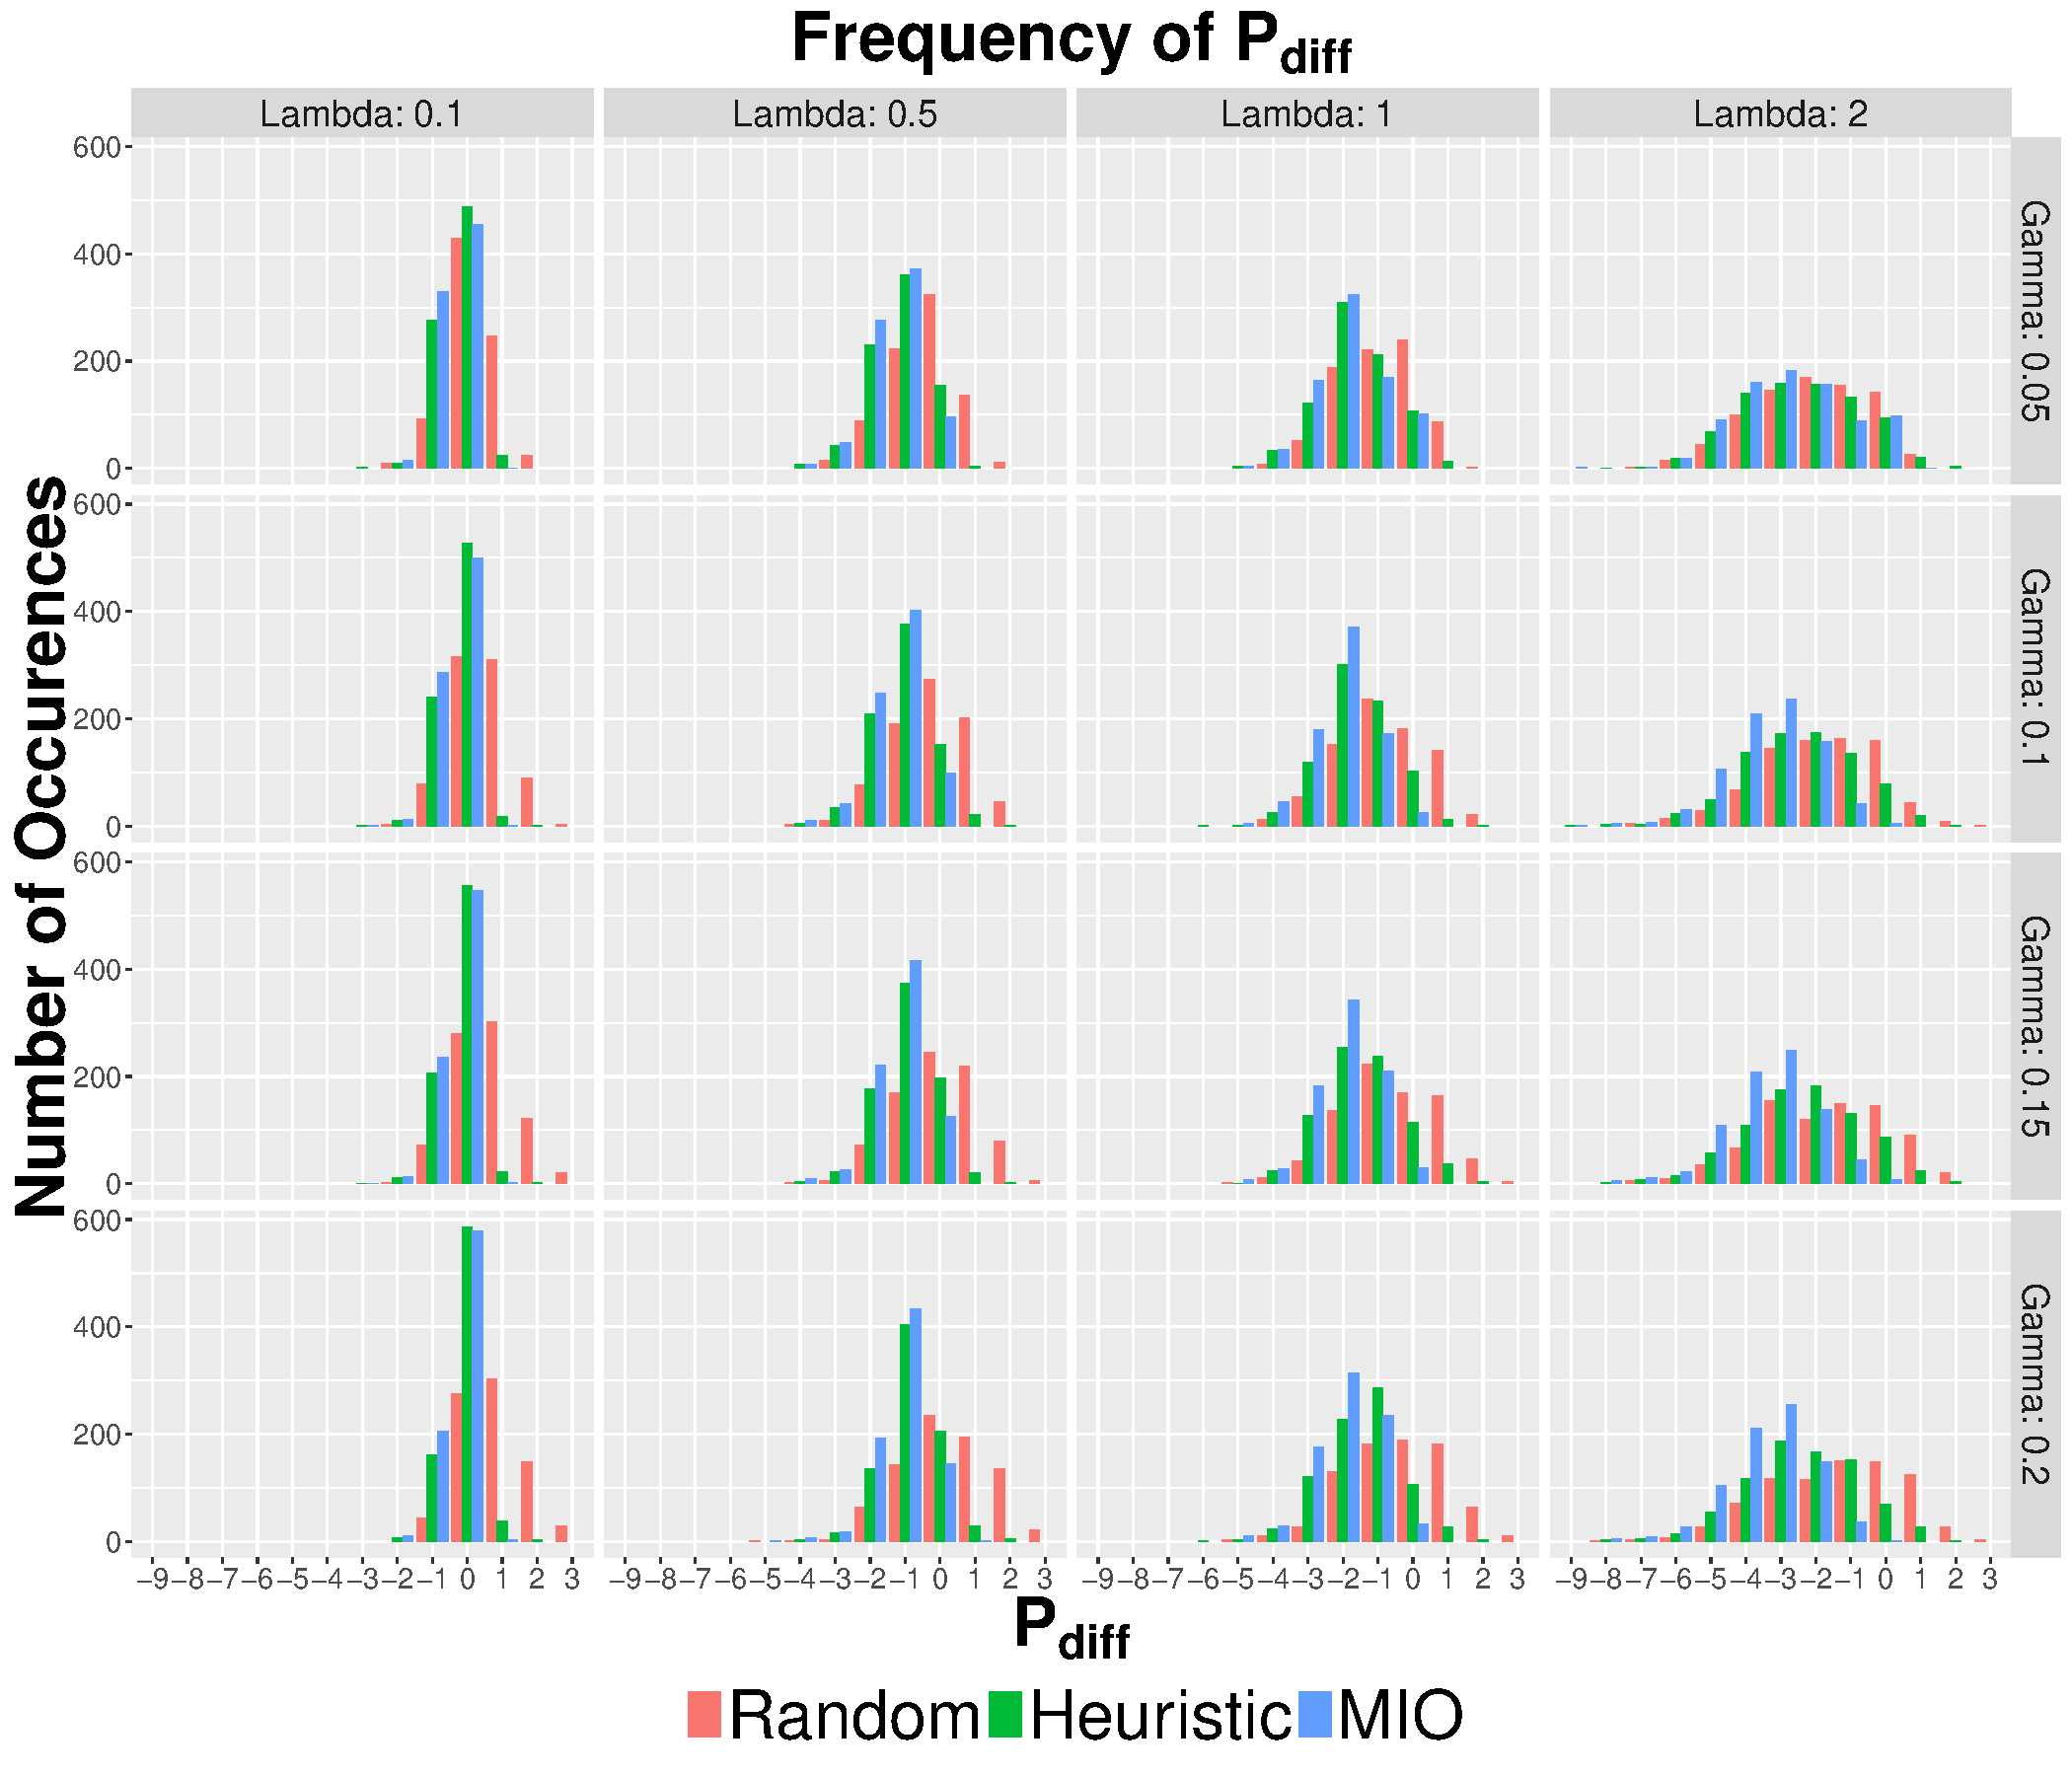
\includegraphics[width=.7\columnwidth]{../Figures/4_8_Histogram}
\end{figure}
\end{frame}

\begin{frame}
\frametitle{Estimating the Number of Targets ($P_{true}=8$)} 
\begin{figure}[ht]
  \centering
  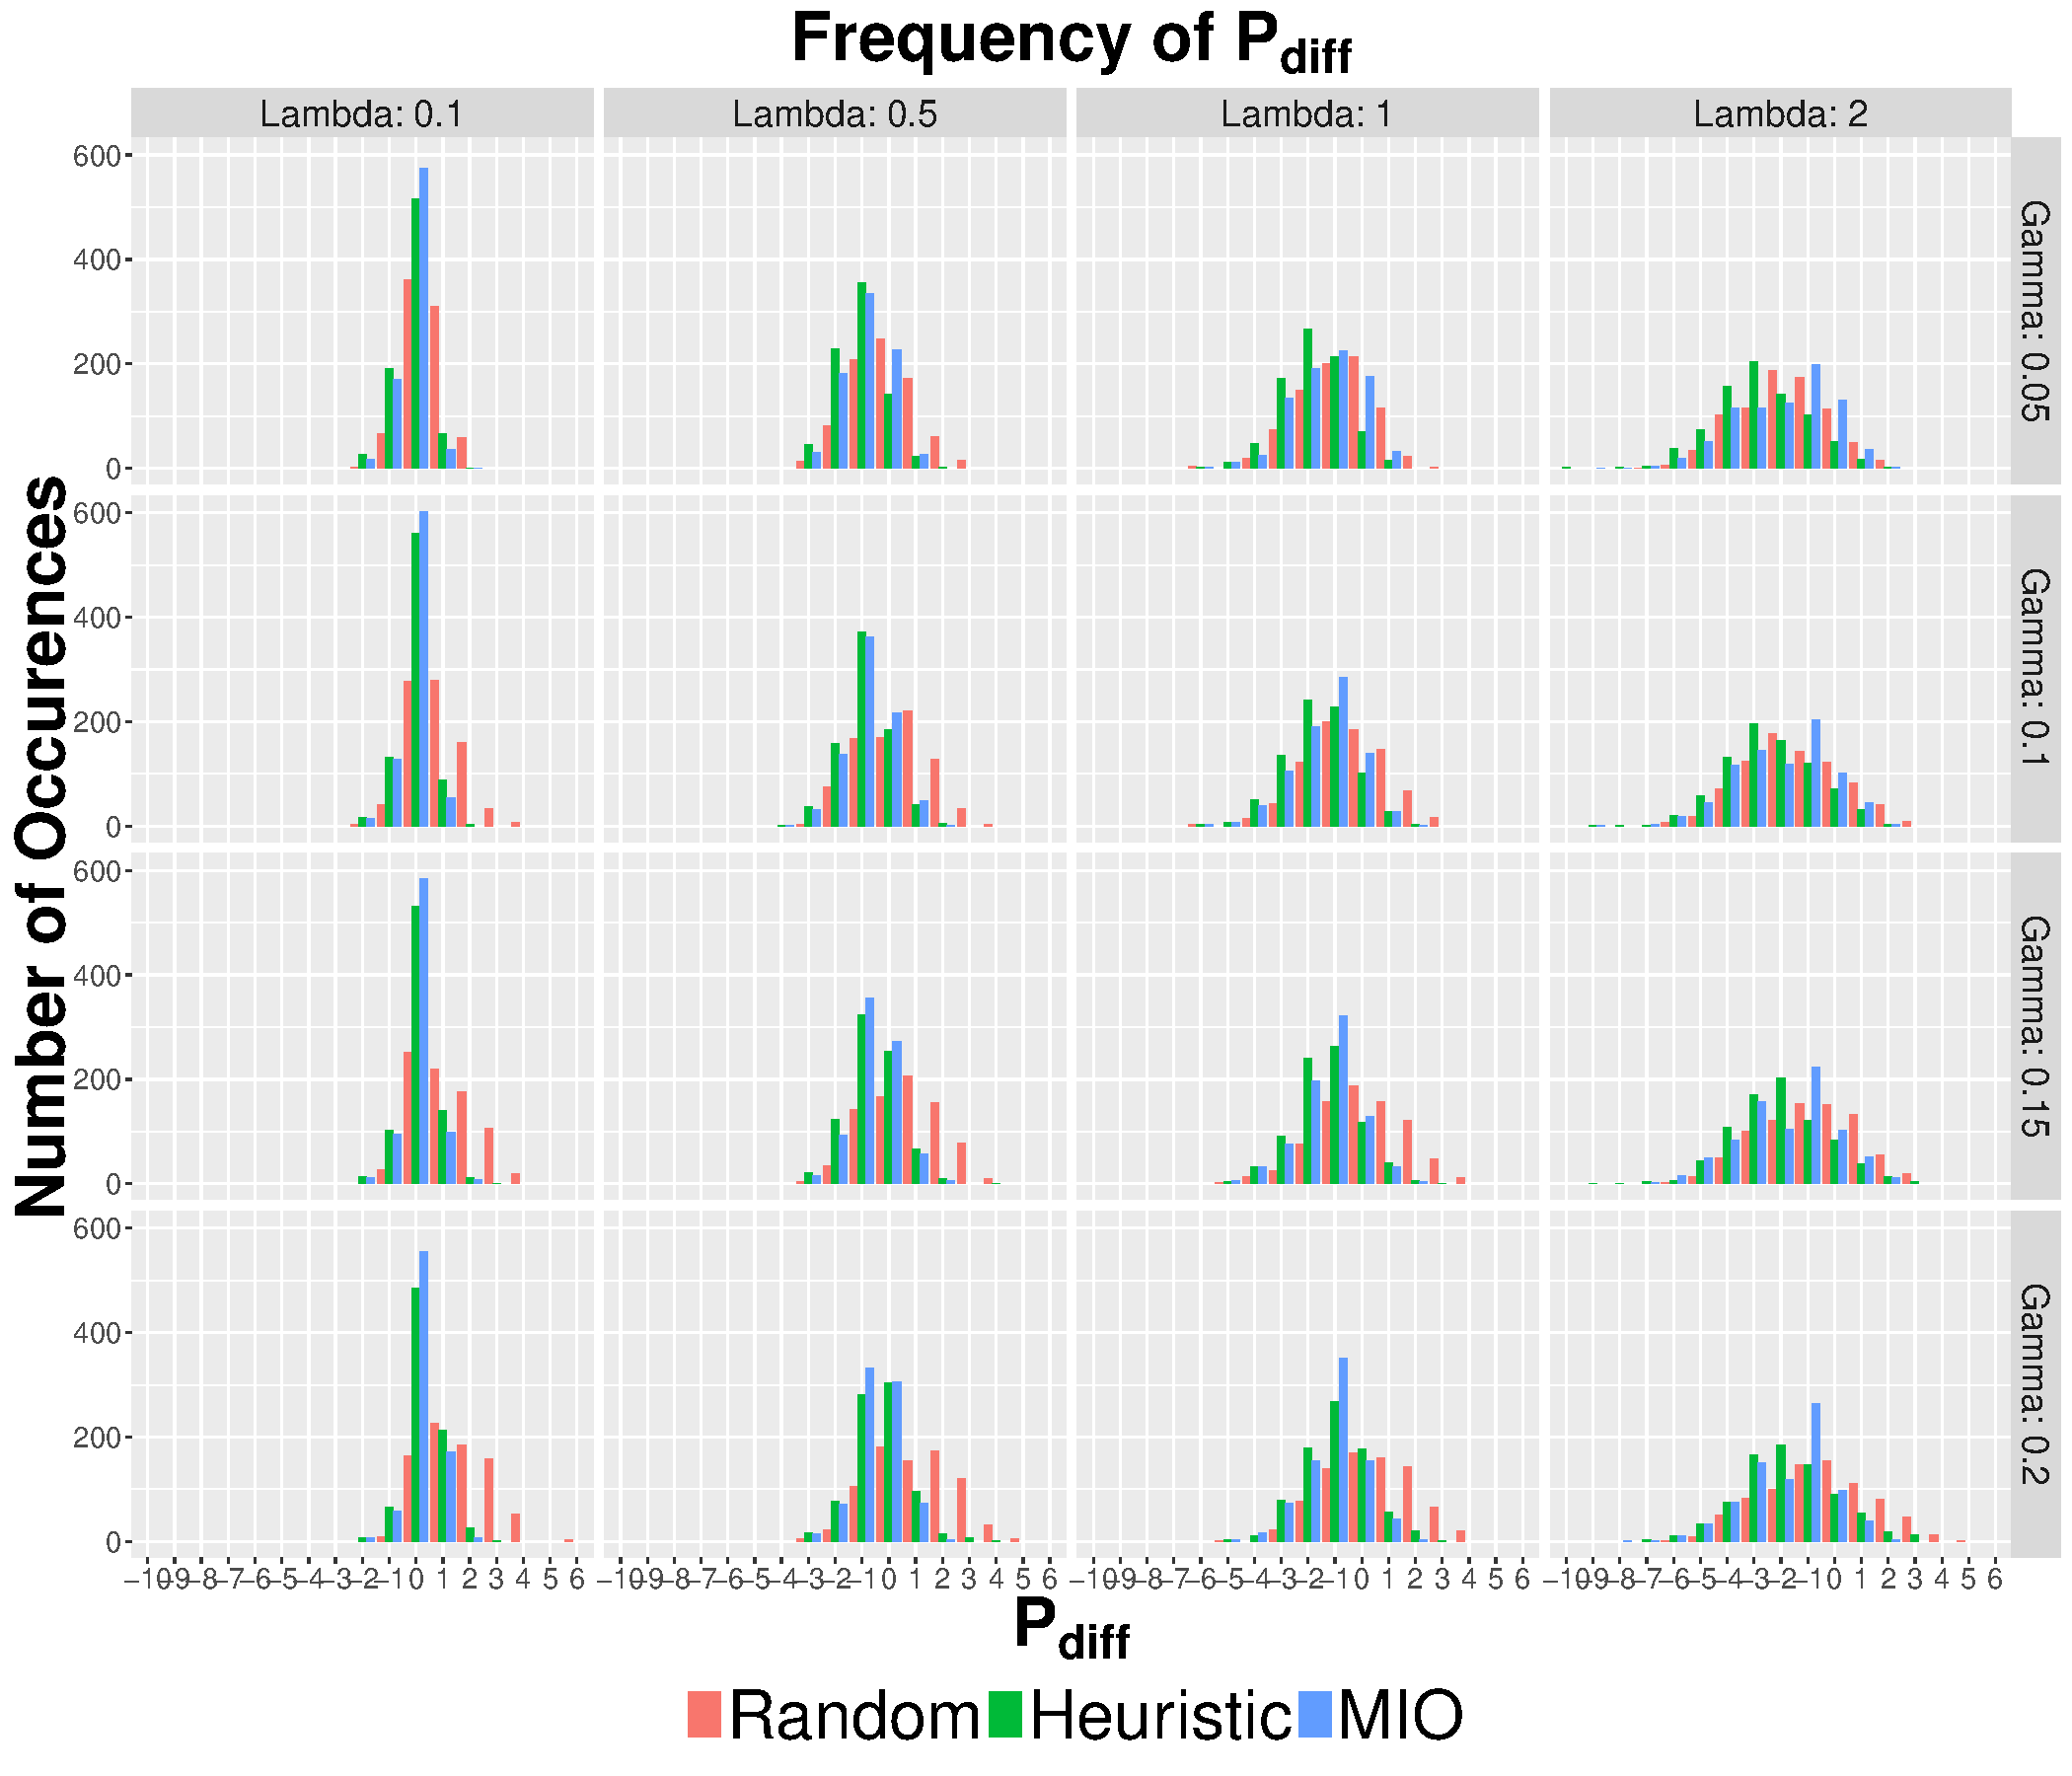
\includegraphics[width=.7\columnwidth]{../Figures/8_8_Histogram}
\end{figure}
\end{frame}

\begin{frame}
\frametitle{Data Association Accuracy ($P_{true}=4$)} 
\begin{figure}[ht]
  \centering
  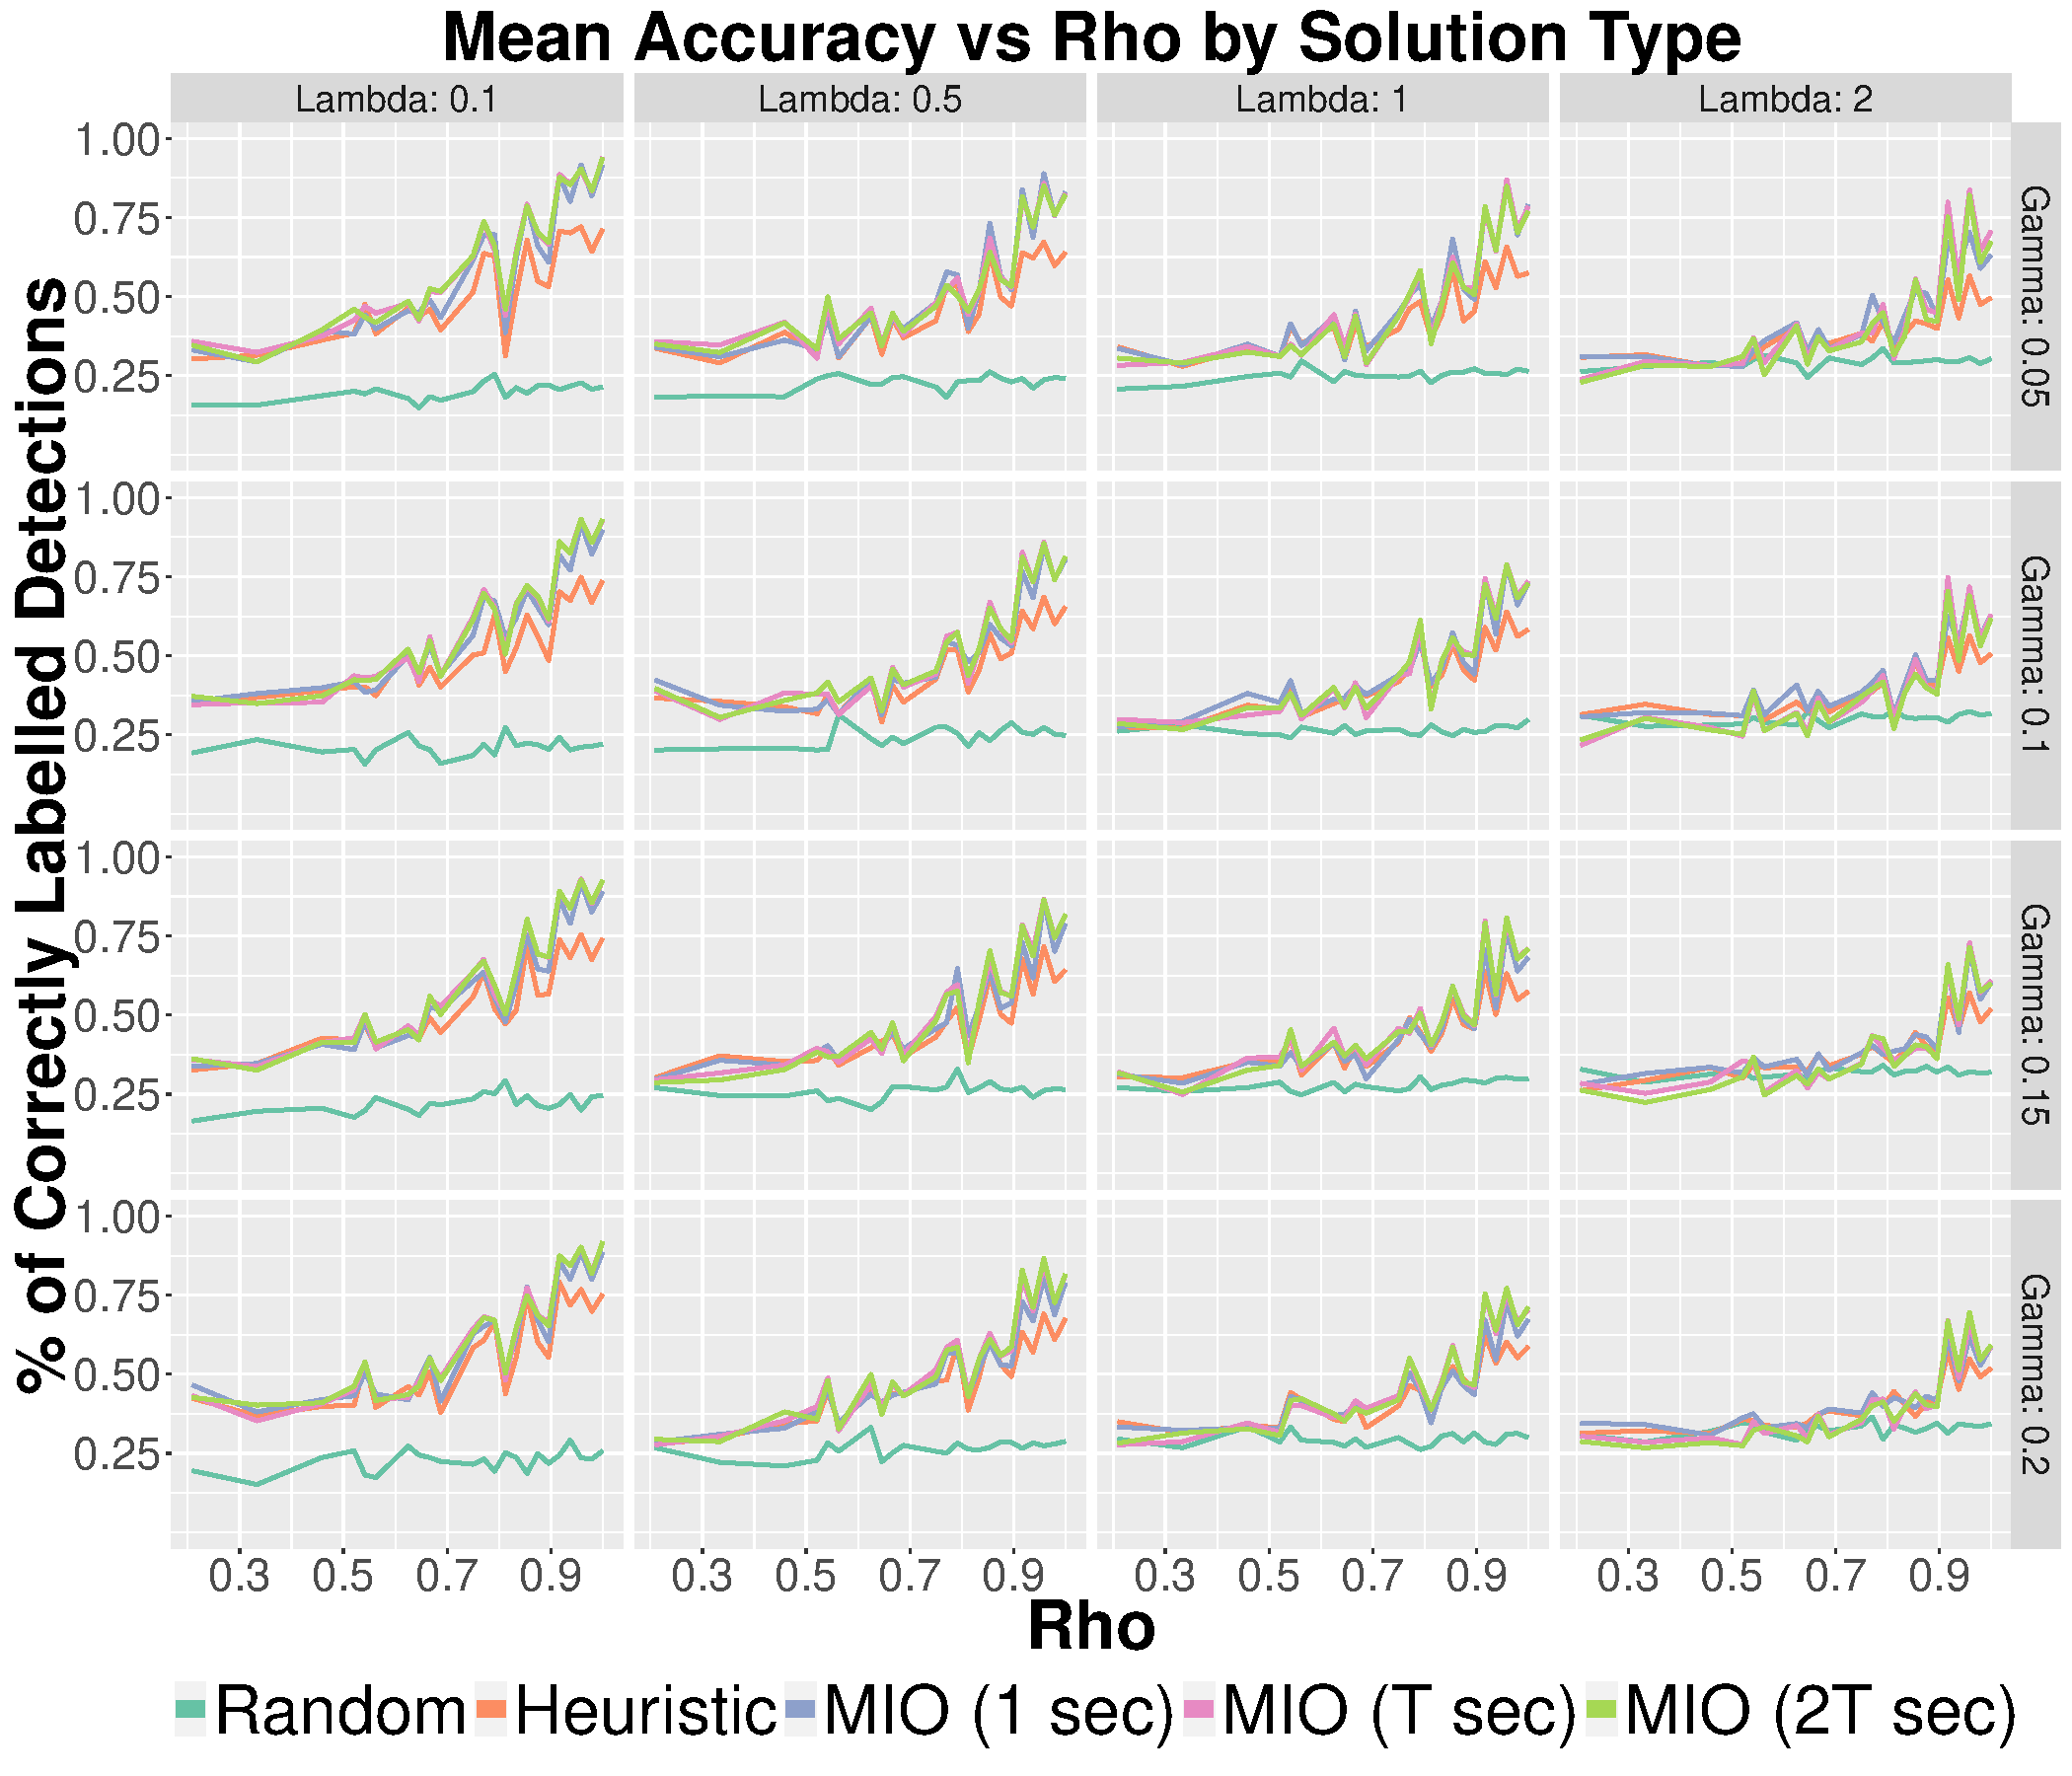
\includegraphics[width=.7\columnwidth]{../Figures/4_8_Accuracy}
\end{figure}
\end{frame}

\begin{frame}
\frametitle{Data Association Accuracy ($P_{true}=8$)} 
\begin{figure}[ht]
  \centering
  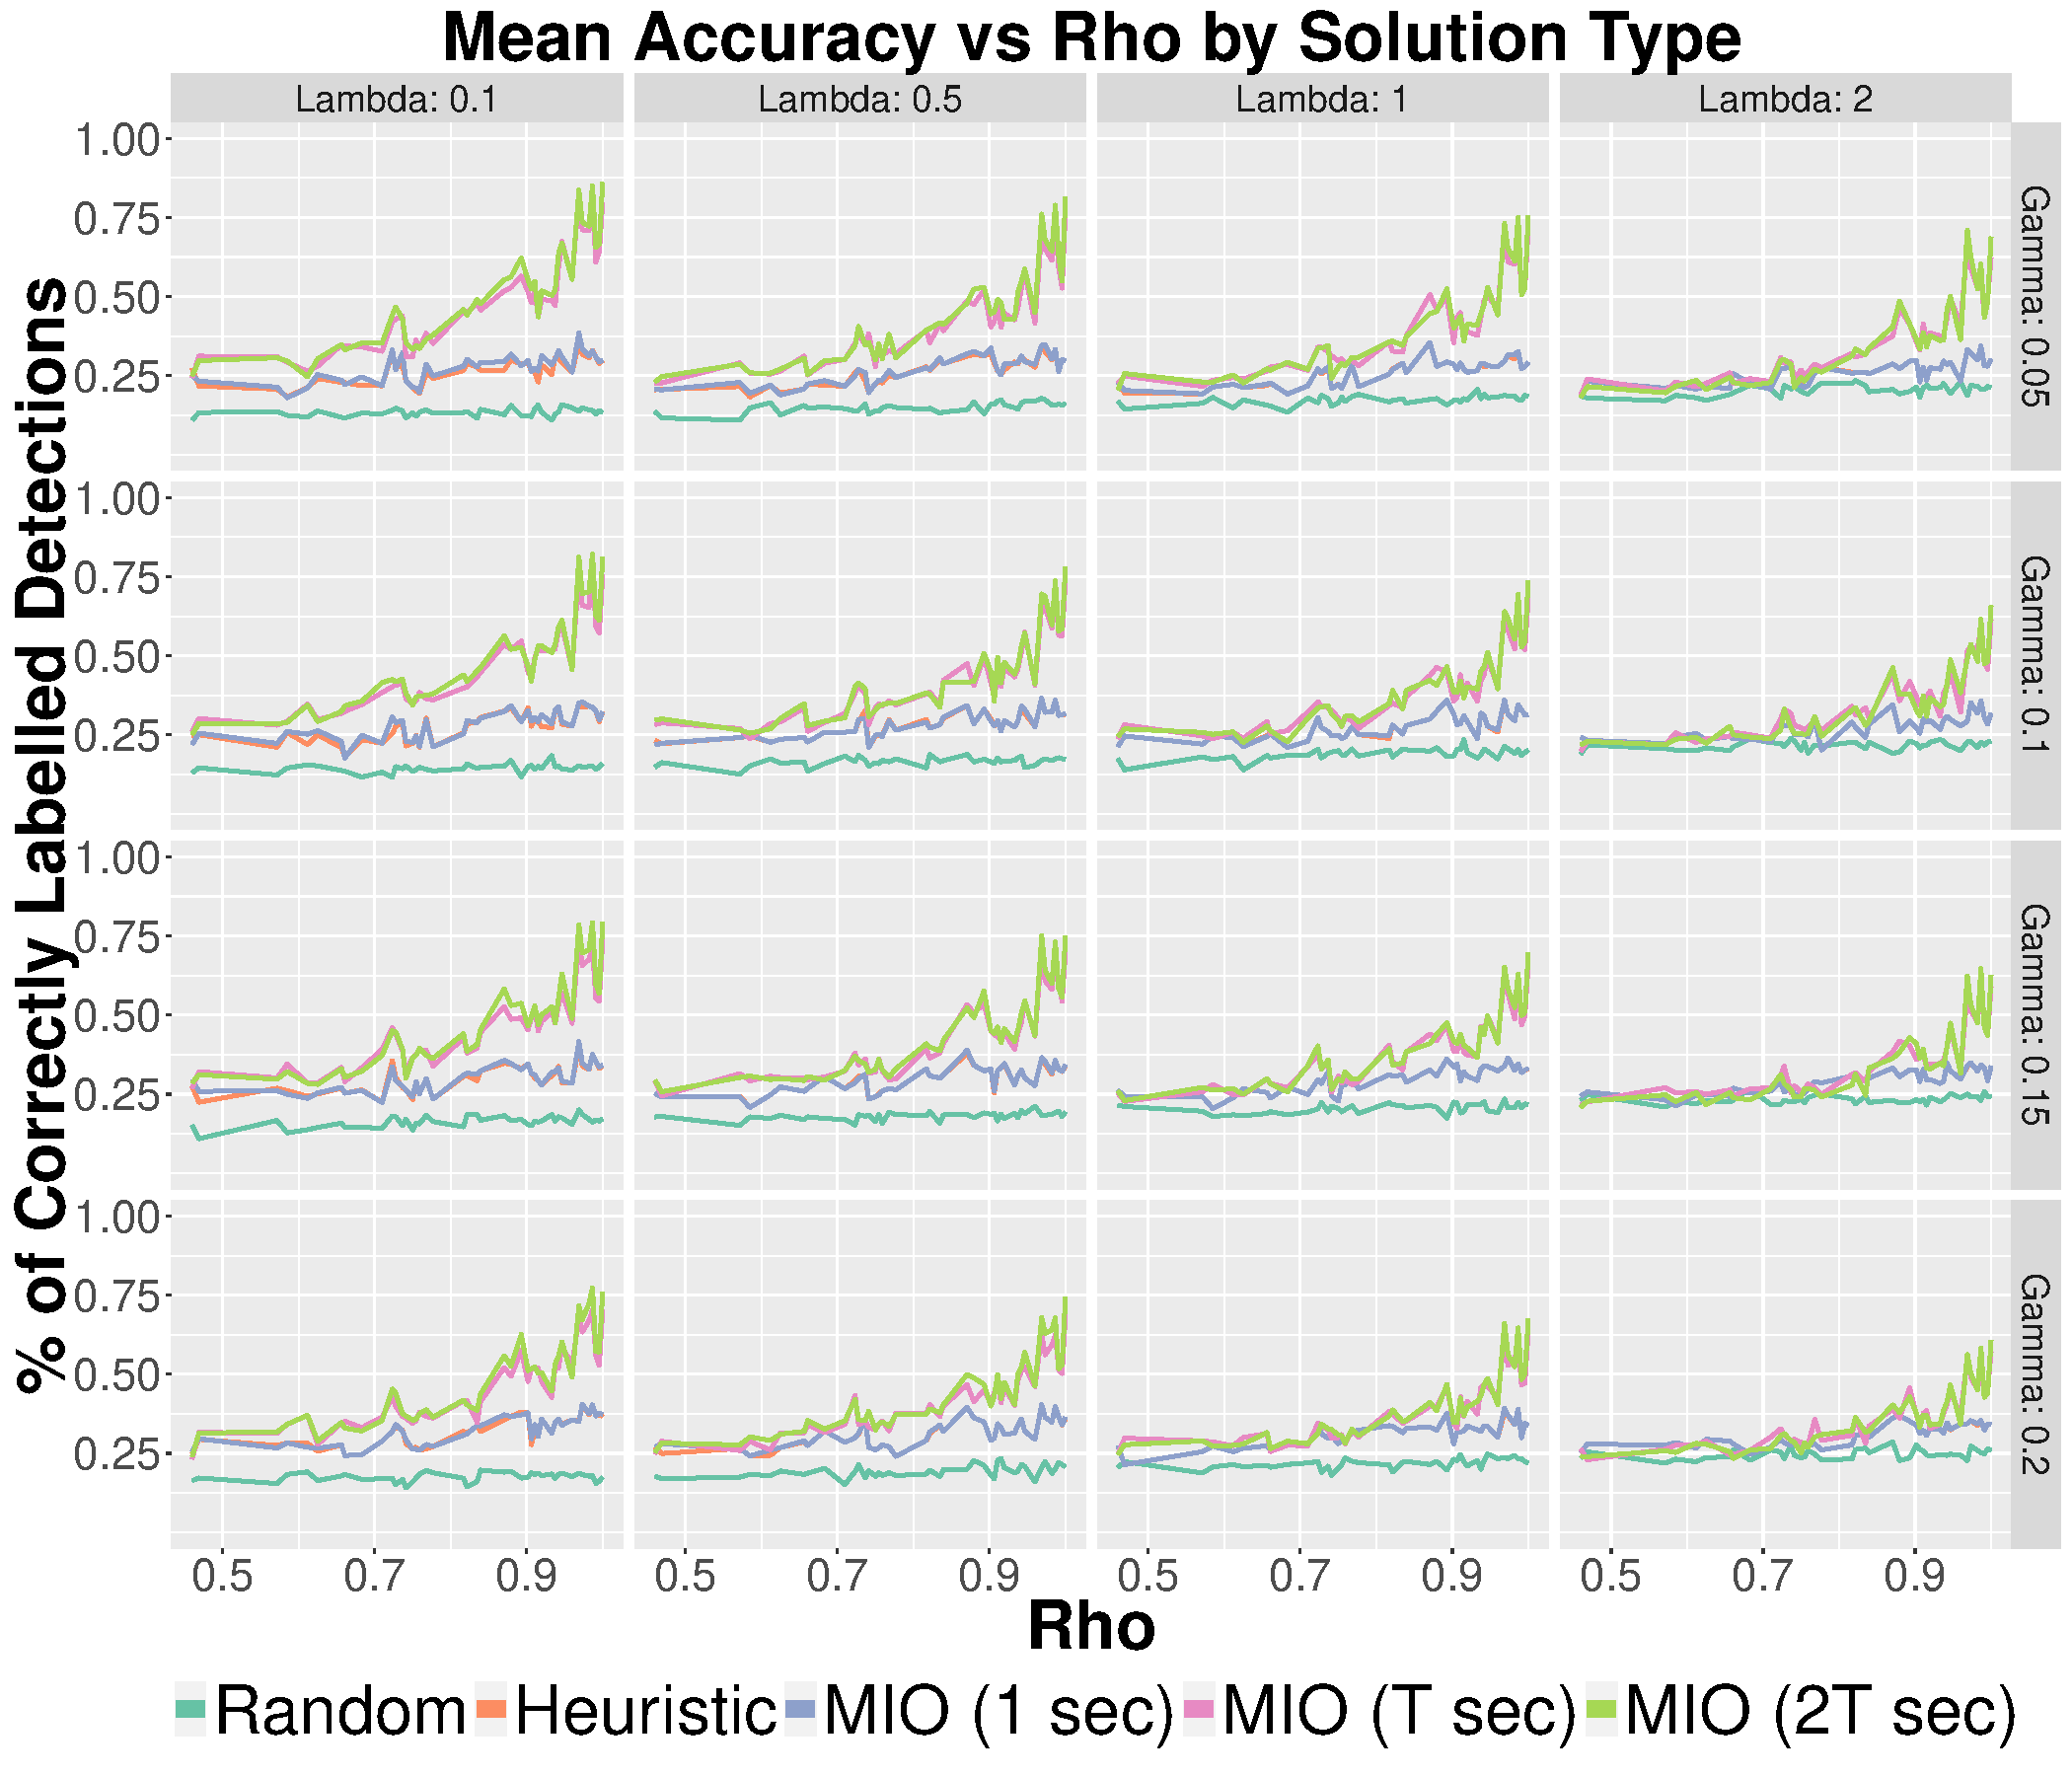
\includegraphics[width=.7\columnwidth]{../Figures/8_8_Accuracy}
\end{figure}
\end{frame}

\begin{frame}
\frametitle{Trajectory Estimation Error ($P_{true}=4$)} 
\begin{figure}[ht]
  \centering
  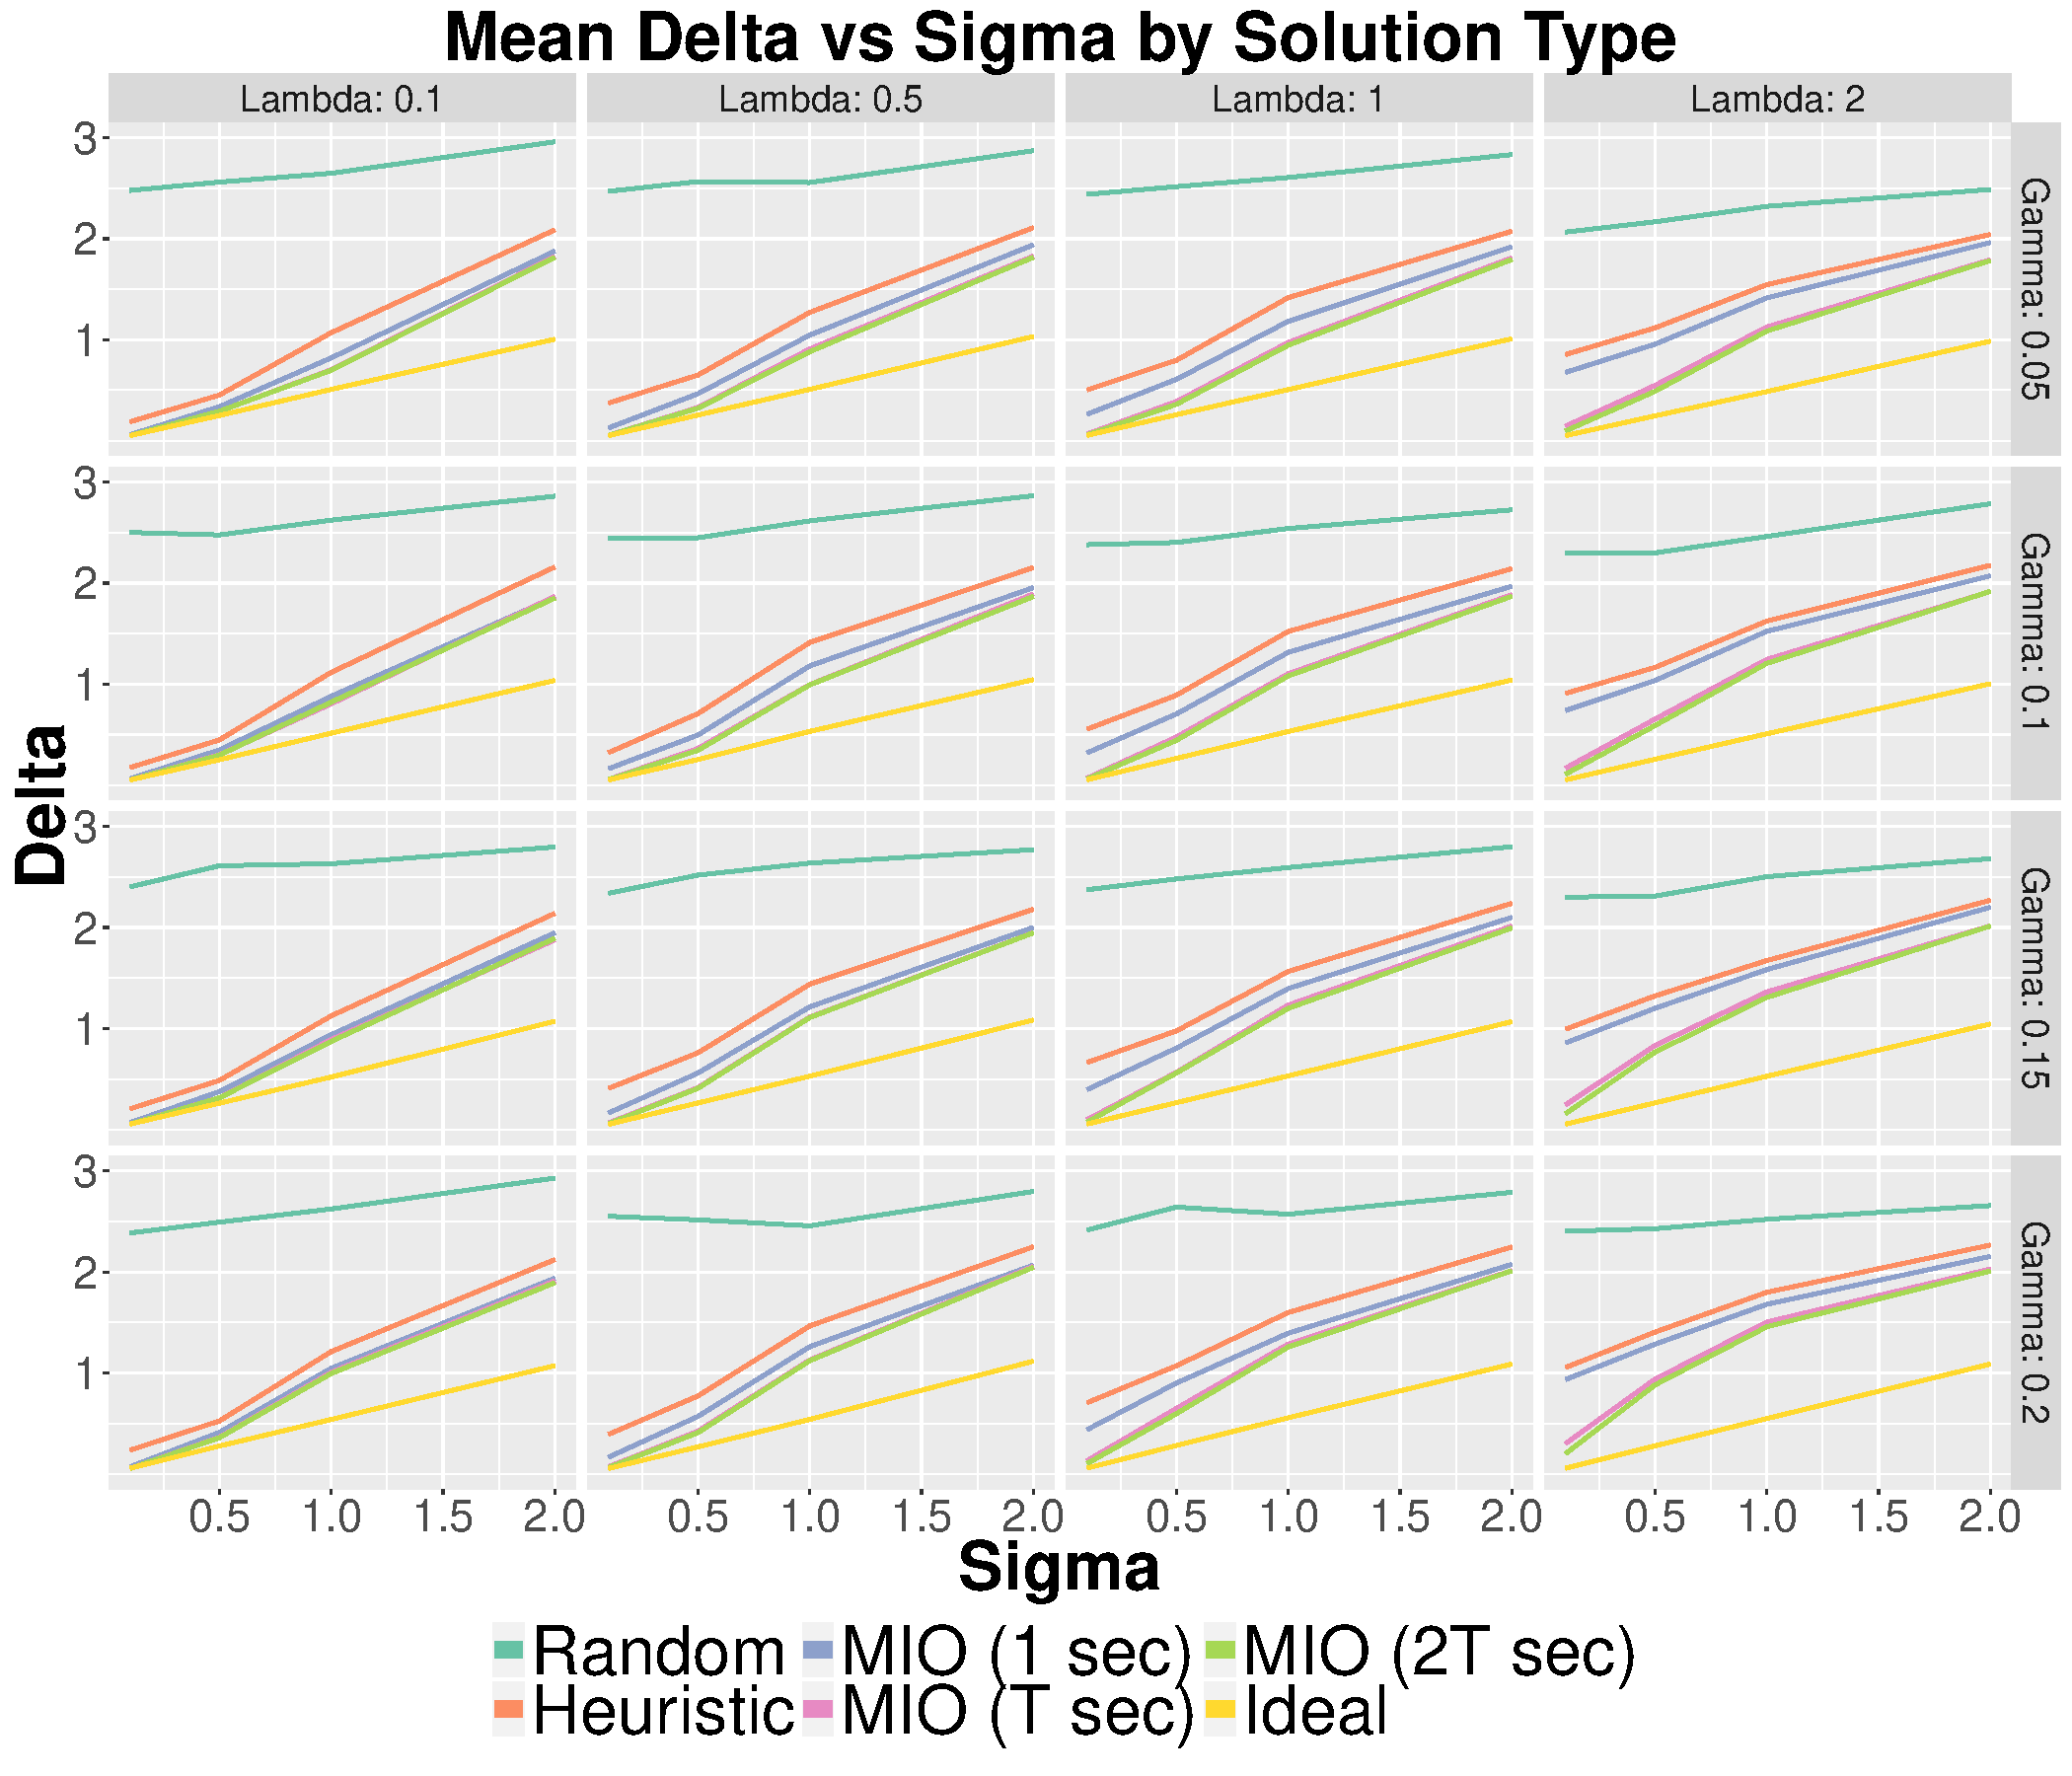
\includegraphics[width=.7\columnwidth]{../Figures/4_8_Delta}
\end{figure}
\end{frame}

\begin{frame}
\frametitle{Trajectory Estimation Error ($P_{true}=8$)} 
\begin{figure}[ht]
  \centering
  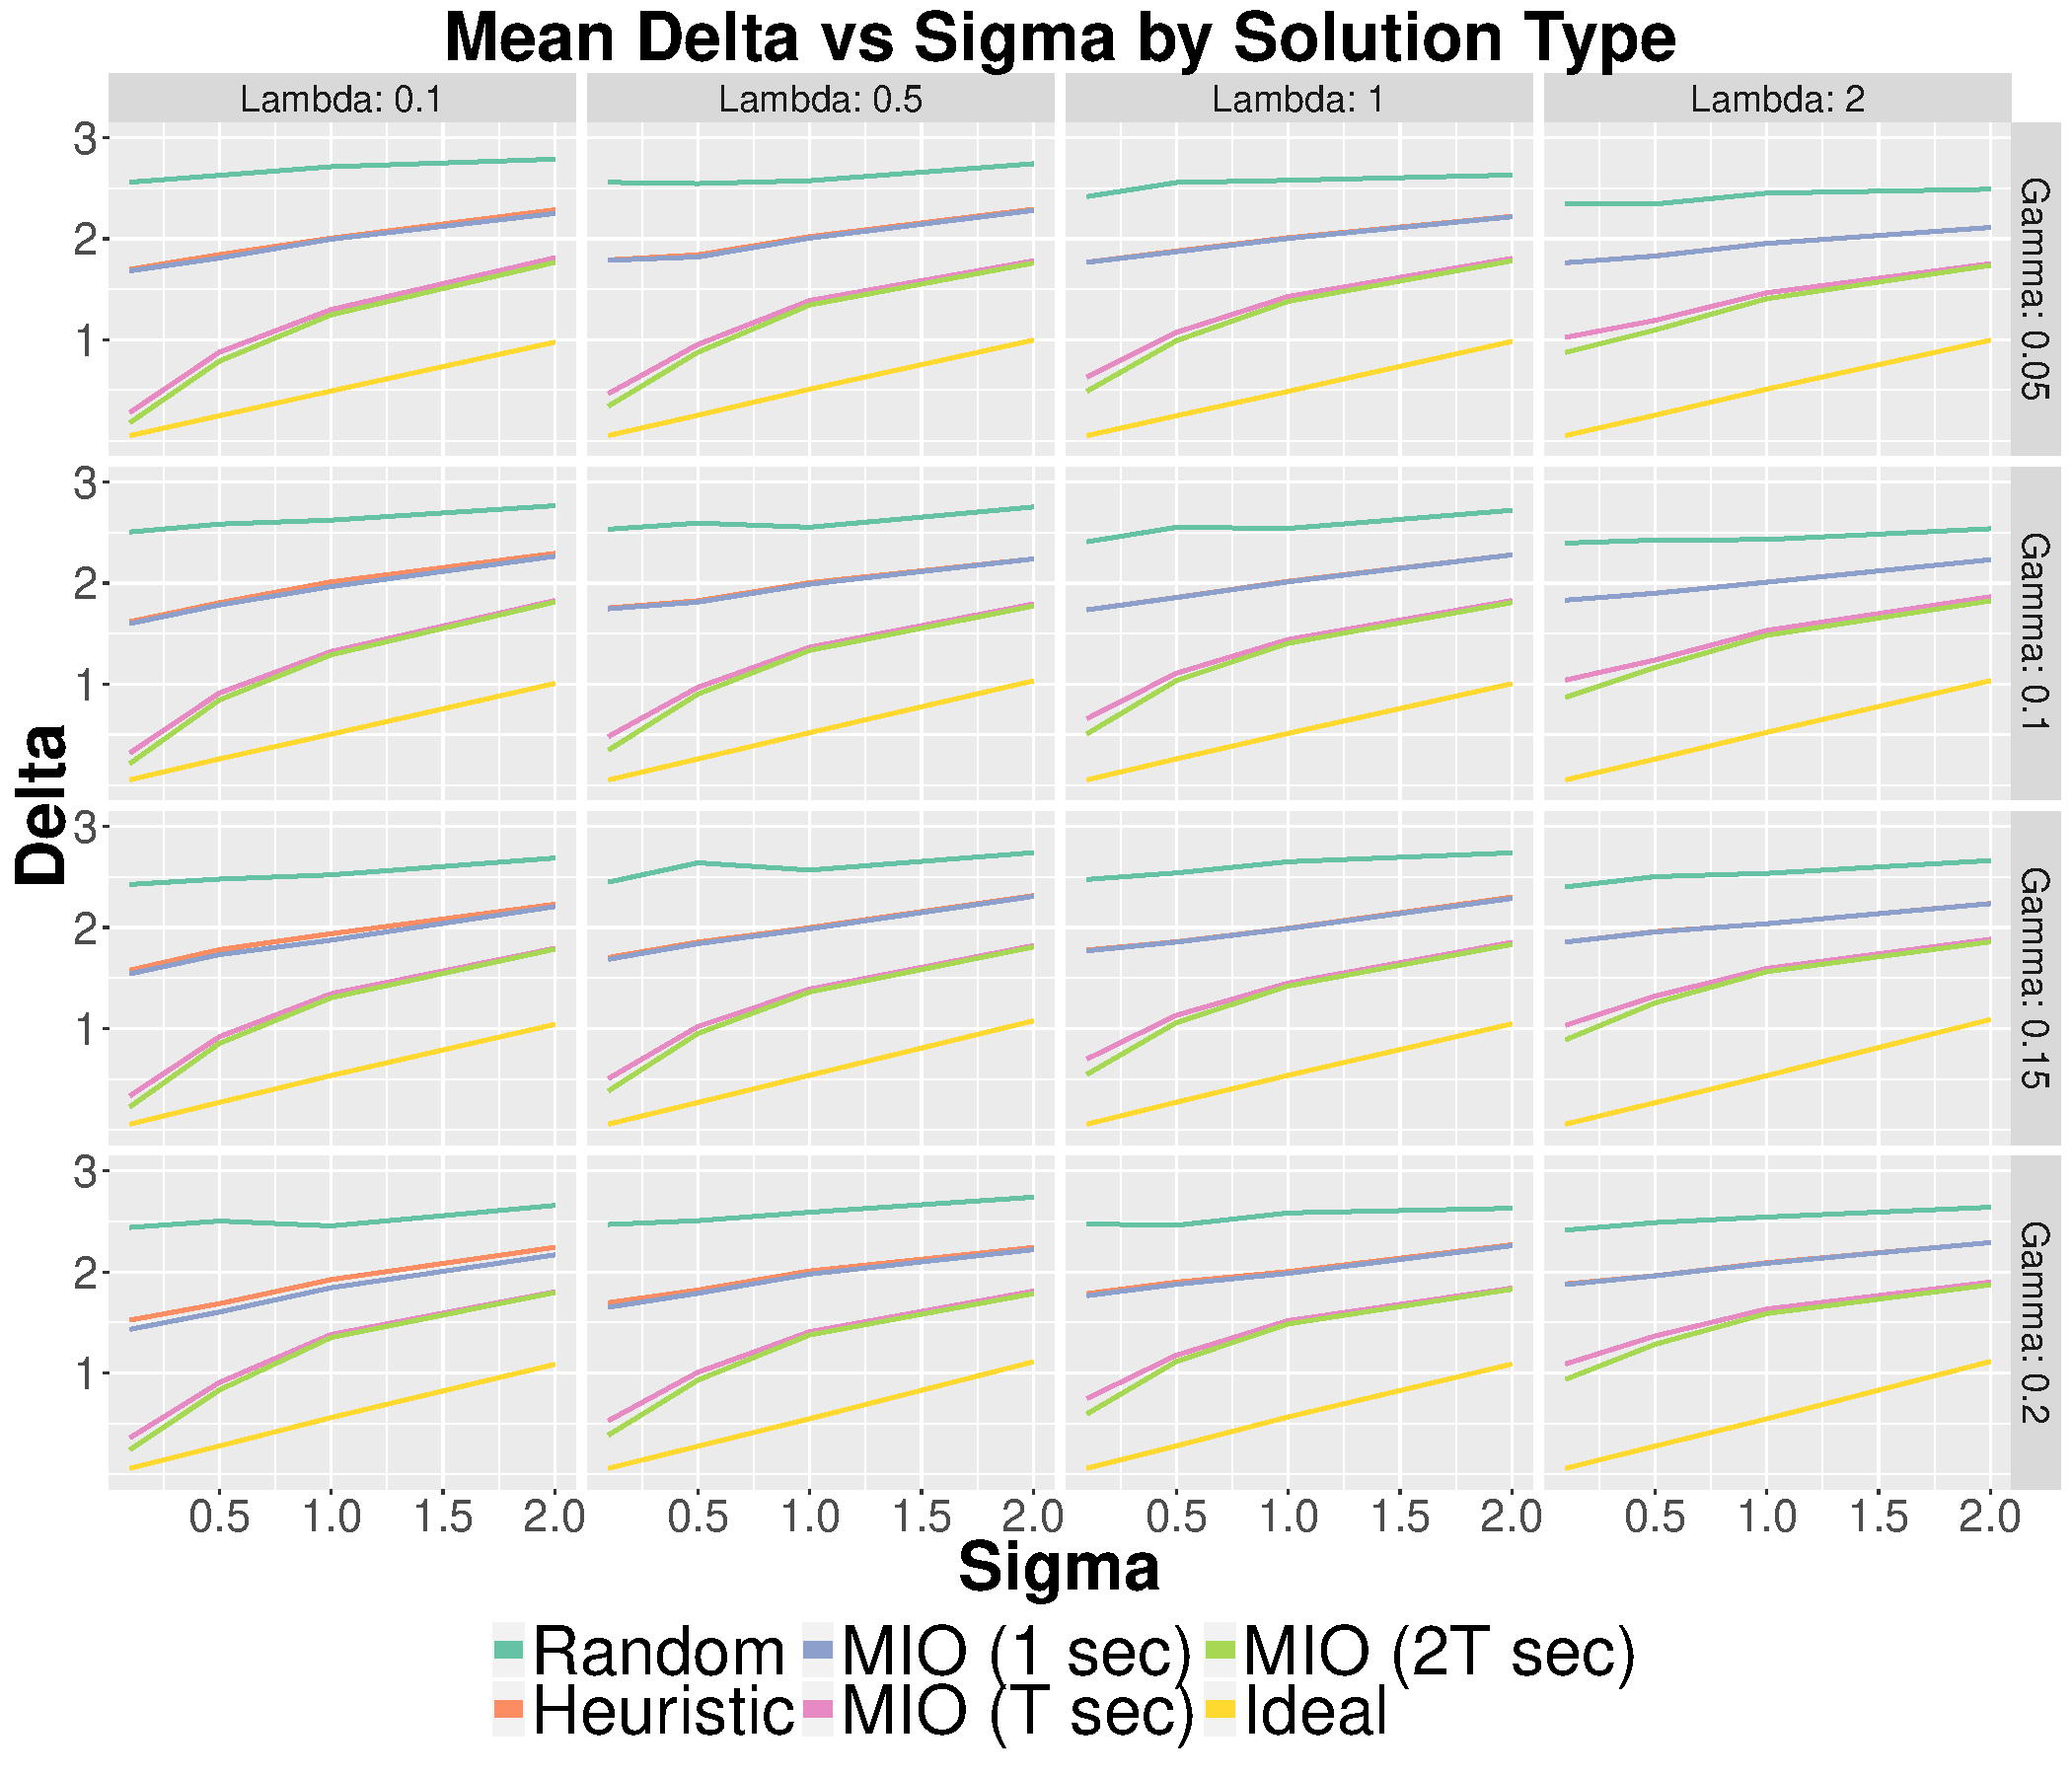
\includegraphics[width=.7\columnwidth]{../Figures/8_8_Delta}
\end{figure}
\end{frame}

\begin{frame}
\frametitle{Summary of cases with detection ambiguity} 

\begin{itemize}
\item Heuristic
\begin{itemize}
\item Slower and scales less efficiently than basic heuristic
\item Run times remain within milliseconds for single starting point
\item Scalability still maintained through parallelization
\end{itemize}
\item MIO
\begin{itemize}
\item Correct estimation of $P$ through parameter tuning.
\item Data association accuracy deteriorates by 5\%-10\% because of detection ambiguity.
\item Overestimating $P$ does not influence quality of trajectory estimation.
\item MIO solution more robust to $\gamma$ than to  $\lambda$.
\end{itemize}
\end{itemize}
\end{frame}

%------------------------------------------------
\section{Summary and Future Work}
%------------------------------------------------
\begin{frame}
\frametitle{Summary of Contributions}
\begin{enumerate}[(i)]
\item Introduced MIO models for solving MTT 
\begin{itemize}
\item Simple and interpretable
\item Requires few assumptions
\item Requires at most two parameters
\end{itemize}
\item Proposed heuristics
\begin{itemize}
\item Very efficient and scalable
\item Useful as warm start for MIO model
\end{itemize}
\item New metrics provide additional insight
\end{enumerate}
\end{frame}

\begin{frame}
\frametitle{Future Work}
\begin{itemize}
\item Extensions to non-linear trajectories
\item More complex penalty functions
\item Extensions to sliding window algorithm
\end{itemize} 
\end{frame}

\appendix
%------------------------------------------------
\section{Penalties}
%------------------------------------------------

\begin{frame}[noframenumbering]
\frametitle{False Alarm Penalty $\theta$}
\begin{table}
\centering
\begin{tabular}{c|m{1cm}m{1cm}m{1cm}m{1cm}}
  \hline
   & \multicolumn{4}{c}{$\sigma$} \\
   \cline{2-5}
   $\lambda$ & 0.1 & 0.5 & 1.0 & 2.0\\
  \hline
  \hline
   0.1 & 1.7 & 2.6 & 3.1 & 3.5 \\
   0.5 & 1.1 & 1.9 & 2.3 & 2.5 \\ 
   1.0 & 0.9 & 1.2 & 1.6 & 1.8 \\ 
   2.0 & 0.5 & 0.9 & 0.9 & 1.0 \\ 
   \hline
\end{tabular}
\caption{False alarm penalties ($\theta$) as a function of $\lambda$ and $\sigma$.}
\end{table}
\end{frame}

\begin{frame}[noframenumbering]
\frametitle{Missed Detection Penalty $\phi$}
\begin{table}\tiny
\centering
\begin{tabular}{cc|cccc}
  \hline
  & & \multicolumn{4}{c}{$\sigma$} \\
  \cline{3-6}
 $\lambda$ & $\gamma$ & 0.1 & 0.5 & 1 & 2 \\ 
  \hline
  \hline
   0.10 & 0.05 & 0.20 & 0.50 & 0.80 & 0.70 \\ 
   0.10 & 0.10 & 0.10 & 0.30 & 0.50 & 0.50 \\ 
   0.10 & 0.15 & 0.10 & 0.20 & 0.40 & 0.40 \\ 
   0.10 & 0.20 & 0.10 & 0.10 & 0.30 & 0.40 \\ 
   0.50 & 0.05 & 0.20 & 0.50 & 0.80 & 0.80 \\ 
   0.50 & 0.10 & 0.20 & 0.30 & 0.50 & 0.60 \\ 
   0.50 & 0.15 & 0.20 & 0.25 & 0.40 & 0.40 \\ 
   0.50 & 0.20 & 0.10 & 0.20 & 0.30 & 0.40 \\ 
   1.00 & 0.05 & 0.30 & 0.70 & 0.80 & 0.80 \\ 
   1.00 & 0.10 & 0.20 & 0.40 & 0.50 & 0.60 \\ 
   1.00 & 0.15 & 0.20 & 0.25 & 0.40 & 0.40 \\ 
   1.00 & 0.20 & 0.10 & 0.20 & 0.30 & 0.40 \\ 
   2.00 & 0.05 & 0.30 & 0.70 & 0.90 & 1.00 \\ 
   2.00 & 0.10 & 0.20 & 0.50 & 0.60 & 0.60 \\ 
   2.00 & 0.15 & 0.20 & 0.25 & 0.40 & 0.50 \\ 
   2.00 & 0.20 & 0.10 & 0.20 & 0.30 & 0.40 \\ 
   \hline
\end{tabular}
\caption{Missed detection penalties ($\phi$) as a function of $\lambda$, $\gamma$, and $\sigma$.}
\end{table}
\end{frame}

%------------------------------------------------
\section{Trajectory Assignment Pairing}
%------------------------------------------------

\begin{frame}[noframenumbering]
\frametitle{$P_{true} = P_{est} = P$}
\begin{align*}
\underset{y_{ij}}{\text{minimize: }} & \sum_{i=1}^{P} \sum_{j=1}^{P} c_{ij}y_{ij}\\
\text{subject to: }	& \sum_{i=1}^{P} y_{ij} = 1 \qquad \forall j = 1,...,P \nonumber \\
				& \sum_{j=1}^{P} y_{ij} = 1 \qquad \forall i = 1,...,P \nonumber \\
				& y_{ij} \in \{0,1\} \quad \forall i = 1,...,P,j = 1,...,P \nonumber
\end{align*}
\end{frame}

\begin{frame}[noframenumbering]
\frametitle{$P_{true} \leq P_{est}$}
\begin{align*}
\underset{y_{ij}}{\text{minimize: }} & \sum_{i=1}^{P_{\text{true}}} \sum_{j=1}^{P_{\text{est}}} c_{ij}y_{ij}\\
\text{subject to: }	& \sum_{i=1}^{P_{\text{true}}} y_{ij} = 1 \qquad \forall j = 1,...,P_{\text{est}} \nonumber \\
				& \sum_{j=1}^{P_{\text{est}}} y_{ij} \leq 1 \qquad \forall i = 1,...,P_{\text{true}}\nonumber \\
				& y_{ij} \in \{0,1\} \quad \forall i = 1,...,P_{\text{true}},j = 1,...,P_{\text{est}}. \nonumber
\end{align*}
\end{frame}

\begin{frame}[noframenumbering]
\frametitle{$P_{true} \geq P_{est}$}
\begin{align*}
\underset{y_{ij}}{\text{minimize: }} & \sum_{i=1}^{P_{\text{true}}} \sum_{j=1}^{P_{\text{est}}} c_{ij}y_{ij}\\
\text{subject to: }	& \sum_{i=1}^{P_{\text{true}}} y_{ij} \leq 1 \qquad \forall  j = 1,...,P_{\text{est}}\nonumber \\
				& \sum_{j=1}^{P_{\text{est}}} y_{ij} = 1 \qquad \forall i = 1,...,P_{\text{true}} \nonumber \\
				& y_{ij} \in \{0,1\} \quad \forall i = 1,...,P_{\text{true}},j = 1,...,P_{\text{est}}. \nonumber
\end{align*}
\end{frame}

%------------------------------------------------
\section{Misc Backup Slides}
%------------------------------------------------
\begin{frame}[noframenumbering]
\frametitle{Heuristic Performance by Number of Starting Points}
\begin{figure}[ht]
  \centering
  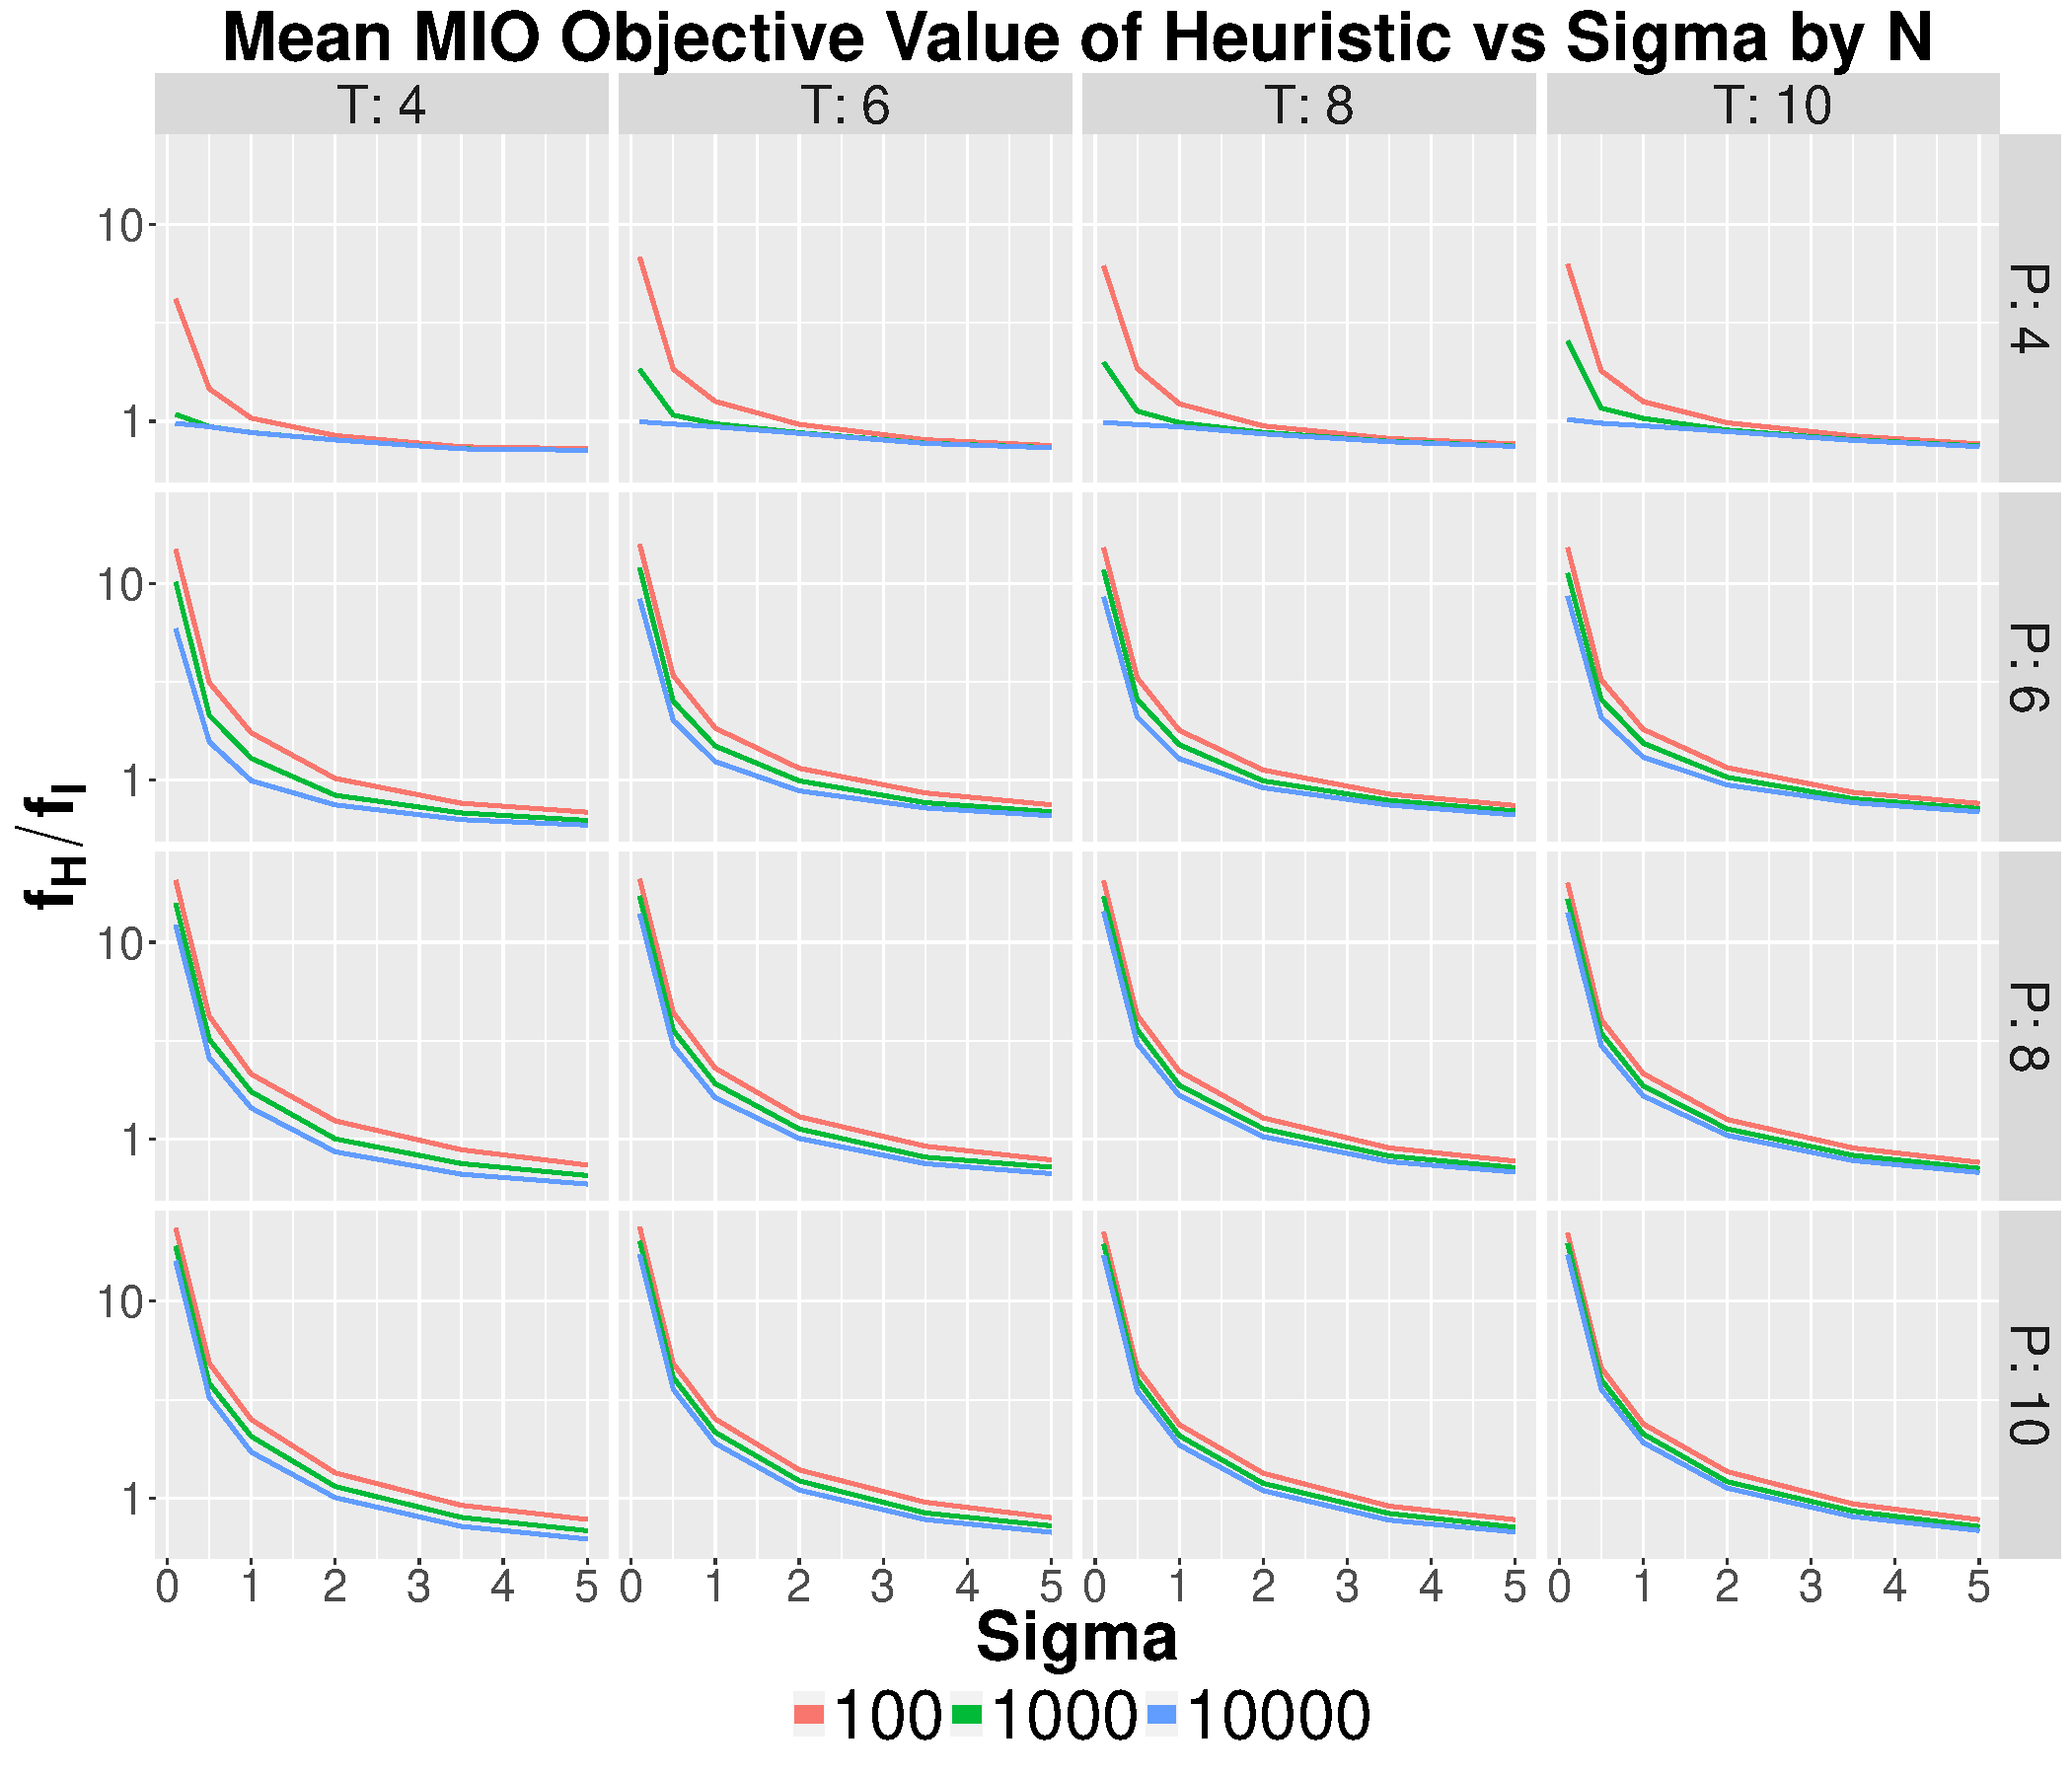
\includegraphics[width=.7\columnwidth]{../Figures/Basic_Heuristic_Objective}
\end{figure}
\end{frame}

\end{document}